\documentclass[a4paper,12pt]{report}

\usepackage{amsmath}
\usepackage{longtable}
\usepackage[hidelinks]{hyperref}
\usepackage{xurl}
\usepackage{indentfirst}
\usepackage{fancyref}
\usepackage{float}
\usepackage{subfigure}
\usepackage[style=numeric,backend=biber]{biblatex}
\addbibresource{./BiB_files/bibliography.bib}
\usepackage[utf8]{inputenc}
\usepackage{graphicx}
\usepackage{tikz}
\usetikzlibrary{arrows.meta, positioning, shapes.geometric, shapes.multipart}
\usepackage{setspace}
\usepackage{titlesec}
\usepackage{lipsum}
\usepackage[romanian]{babel}
\usepackage{xspace}
\usepackage{csquotes}
\usepackage{fontspec}

\setlength{\emergencystretch}{3em}
\sloppy


%\pdfminorversion=6
\setmainfont[Path = fonts/,
 AutoFakeSlant=0.3,
 Extension = .otf,
 UprightFont = UTSans-Regular,
 BoldFont = UTSans-Medium,
 ItalicFont=UTSans-Regular,
 BoldItalicFont=UTSans-Medium
 ]{UTSans}

\begin{document}

\include{./TeX_files/cover}
\begin{titlepage}
	
	\vspace*{-3cm}
	\hspace{-2cm}
	\begin{minipage}{0.65\textwidth}
		
\includegraphics[width=\textwidth]{./images/Logo-UT-MI-SPOT-RO}
	\end{minipage}%
	\hfill
	\begin{minipage}{0.35\textwidth}
		\begin{flushright}
			{\large Programul de studii \par}
			{\large Informatică Aplicată}
		\end{flushright}
	\end{minipage}

	\begin{center}
		\Huge

		\vspace{2cm}

		\textbf{LUCRARE DE LICENȚĂ}

		\vspace{1cm}

		\LARGE
		BeeSmart: aplicație mobilă dedicată apiculturii de precizie pentru digitalizarea și optimizarea managementului stupinelor

		\vfill

		\Large
		\begin{tabular}{ll}
				\textbf{Absolvent:}&Lixandru Valentina-Mariana\\
			\textbf{Coordonator:}&Lect. Dr. Nănău Corina-Ștefania
		\end{tabular}

		\vfill

		\Large
		Brașov\\
		Iunie 2026

	\end{center}
\end{titlepage}


\tableofcontents
% Fără spațiu vertical între capitole în lista de figuri
\begingroup
\renewcommand*{\addvspace}[1]{}
\listoffigures
\endgroup

\chapter*{Listă de abrevieri și termeni}
\addcontentsline{toc}{chapter}{Listă de abrevieri și termeni}

Tabelele de mai jos rezumă abrevierile tehnice și termenii din domeniul apicol folosiți pe parcursul lucrării.

\section*{Abrevieri și acronime}

\begin{longtable}{@{}p{2.6cm} p{10.6cm}@{}}
\textbf{Abreviere} & \textbf{Semnificație} \\
\hline
\endfirsthead
\textbf{Abreviere} & \textbf{Semnificație} \\
\hline
\endhead
AI & Inteligență artificială: domeniul care urmărește construirea de sisteme capabile să execute sarcini ce necesită în mod normal inteligență umană, precum recunoașterea imaginilor. \\
API & (\textit{Application Programming Interface}) Contractul prin care două programe comunică între ele: setul de funcții, puncte de acces și reguli prin care o aplicație poate folosi serviciile alteia. \\
CNN & (\textit{Convolutional Neural Network}) Rețea neuronală specializată în prelucrarea imaginilor, care învață singură tipare vizuale prin filtre aplicate succesiv asupra pixelilor. \\
CRUD & Acronim pentru cele patru operații fundamentale asupra datelor: creare, citire, actualizare și ștergere (\textit{Create, Read, Update, Delete}). \\
DAO & (\textit{Data Access Object}) Componentă software care concentrează și izolează codul de acces la baza de date față de restul aplicației. \\
DI & (\textit{Dependency Injection}) Mecanism prin care un obiect primește din exterior componentele de care depinde, în loc să le construiască singur. \\
DTO & (\textit{Data Transfer Object}) Obiect simplu, fără logică de business, folosit pentru a transporta date prin rețea sau între straturile unei aplicații. \\
EF Core & (\textit{Entity Framework Core}) Instrumentul Microsoft de mapare obiect-relațională pentru .NET, care permite lucrul cu baza de date prin obiecte C\# și generează automat comenzile SQL. \\
FK & Cheie externă (\textit{Foreign Key}): coloană care leagă o entitate de cheia primară a alteia și materializează relațiile dintre tabele. \\
HTTP / HTTPS & Protocolul de comunicație al aplicațiilor web; varianta HTTPS adaugă un strat de criptare peste HTTP. \\
IoT & (\textit{Internet of Things}) Rețea de dispozitive fizice echipate cu senzori și conectate la internet, care colectează și schimbă date. \\
IP & (\textit{Internet Protocol}) Adresa numerică ce identifică un dispozitiv într-o rețea. \\
JSON & (\textit{JavaScript Object Notation}) Format text, ușor de citit atât de oameni, cât și de programe, folosit pe scară largă pentru schimbul de date. \\
JVM & (\textit{Java Virtual Machine}) Mediul de execuție pe care rulează codul compilat Java și Kotlin. \\
JWT & (\textit{JSON Web Token}) Token semnat criptografic care atestă identitatea unui utilizator autentificat. \\
MVVM & (\textit{Model–View–ViewModel}) Șablon arhitectural care separă afișarea (View) de logica de prezentare (ViewModel) și de date (Model). \\
ORM & (\textit{Object-Relational Mapping}) Tehnică prin care obiectele din cod sunt puse în corespondență cu tabelele unei baze de date relaționale. \\
PDF & (\textit{Portable Document Format}) Format de document independent de platformă, destinat vizualizării și tipăririi consecvente. \\
PK & Cheie primară (\textit{Primary Key}): coloana care identifică unic fiecare rând dintr-un tabel. \\
QR & (\textit{Quick Response}) Cod de bare bidimensional care poate fi citit rapid cu camera unui telefon. \\
ReLU & (\textit{Rectified Linear Unit}) Funcție de activare folosită în rețelele neuronale, care păstrează valorile pozitive și anulează valorile negative. \\
REST & (\textit{Representational State Transfer}) Stil de proiectare a serviciilor web, organizat în jurul resurselor și al metodelor HTTP standard. \\
SDK & (\textit{Software Development Kit}) Ansamblu de instrumente, biblioteci și documentație pentru dezvoltarea aplicațiilor pe o anumită platformă. \\
SMTP & (\textit{Simple Mail Transfer Protocol}) Protocolul standard folosit pentru trimiterea mesajelor de e-mail. \\
SQL & (\textit{Structured Query Language}) Limbajul standard de interogare și manipulare a bazelor de date relaționale. \\
TTL & (\textit{Time To Live}) Durata cât o valoare rămâne validă, de exemplu într-un cache, înainte de a fi considerată expirată. \\
UI & (\textit{User Interface}) Interfața grafică prin care utilizatorul interacționează cu o aplicație. \\
URL / URI & Adresa care identifică și localizează o resursă; un „Data URI" conține resursa (de exemplu, o imagine) codată direct în adresă. \\
UUID & (\textit{Universally Unique Identifier}) Identificator de 128 de biți, practic unic la nivel global, folosit pentru a eticheta entități fără coordonare centrală. \\
\end{longtable}

\section*{Termeni din domeniul apicol}

\begin{longtable}{@{}p{2.6cm} p{10.6cm}@{}}
\textbf{Termen} & \textbf{Explicație} \\
\hline
\endfirsthead
\textbf{Termen} & \textbf{Explicație} \\
\hline
\endhead
Apicultură de precizie & Direcție de gestionare a coloniilor pe baza datelor colectate, pentru decizii mai bune și pierderi reduse. \\
Botcă & Celulă specială în care este crescută o nouă matcă; prezența botcilor cu ouă este un semnal de pregătire a roirii. \\
Compactitatea puietului & Măsură a uniformității cu care sunt ocupate celulele cu puiet pe o ramă; un puiet compact, fără goluri, indică de regulă o matcă sănătoasă. \\
Cules & Perioada în care albinele adună nectar și polen de la plantele melifere. \\
DeepBee & Metoda din literatură pentru detecția și clasificarea automată a celulelor de fagure, integrată ca serviciu AI în BeeSmart. \\
Fagure & Structura de celule hexagonale din ceară, folosită pentru creșterea puietului și depozitarea hranei. \\
Inspecție & Operația de verificare a unui stup, în care apicultorul observă și notează starea familiei. \\
Matcă (regină) & Singura femelă fertilă a coloniei, responsabilă de ponta ouălor. \\
Nosema & Boală a albinelor adulte cauzată de paraziți interni (microsporidii); apare printre tipurile de tratament înregistrate în BeeSmart. \\
Puiet & Totalitatea stadiilor de dezvoltare a albinelor în celule: ouă, larve și puiet căpăcit. \\
Puiet căpăcit & Celulele cu larve acoperite cu un căpăcel de ceară, în stadiul de transformare în albine adulte. \\
Ramă & Cadrul de lemn pe care albinele construiesc fagurele; unitate de bază în evaluarea unui stup. \\
Roire & Procesul natural prin care o parte din colonie pleacă împreună cu matca pentru a forma o familie nouă. \\
Stup & Adăpostul unei familii de albine; în aplicație, entitatea \texttt{Hive}. \\
Stupină & Ansamblul de stupi al unui apicultor, amplasat într-o locație; în aplicație, entitatea \texttt{Apiary}. \\
Urdiniș & Deschiderea de la baza stupului prin care intră și ies albinele. \\
\textit{Varroa} & Acarianul parazit \textit{Varroa destructor}, una dintre principalele cauze ale slăbirii coloniilor; tratamentele împotriva sa sunt urmărite în aplicație. \\
\end{longtable}


\chapter{Introducere}
\label{chap:introducere}

\section{Contextul general al lucrării}

Apicultura este o activitate în care observația directă, memoria intervențiilor și ritmul sezonier al naturii se întâlnesc într-un mod foarte concret. O familie de albine nu poate fi evaluată numai printr-o valoare numerică izolată, ci printr-un istoric: când a fost verificată matca, ce cantitate de puiet exista la ultima inspecție, ce tratament a fost aplicat, cum au evoluat rezervele de hrană și dacă vremea a permis sau nu zborul albinelor. În practică, aceste informații sunt adesea notate în agende, foi separate, aplicații generale de notițe sau fișiere tabelare. Soluțiile de acest tip pot funcționa pentru un număr mic de stupi, dar devin greu de urmărit atunci când apicultorul gestionează mai multe stupine, perioade diferite de tratament și inspecții repetate pentru fiecare stup.

Lucrarea de față pornește de la această nevoie practică și prezintă proiectarea aplicației BeeSmart, o soluție mobilă pentru management apicol. Aplicația este construită în jurul unui client Android, al unui backend ASP.NET Core, al unei baze de date relaționale (SQL Server în mediul de dezvoltare și Azure SQL Database în varianta publică) și al unui serviciu AI inspirat de modelul DeepBee. Ideea centrală este că utilizatorul trebuie să poată lucra în teren, nu doar într-un mediu ideal de birou. Din acest motiv, BeeSmart este proiectată cu o strategie offline-first: datele introduse fără conexiune la internet sunt salvate local, iar sincronizarea cu serverul este realizată ulterior.

Aplicația BeeSmart include funcționalități pentru administrarea stupinelor și a stupilor, completarea inspecțiilor, înregistrarea tratamentelor, extracțiilor și task-urilor, atașarea fotografiilor, afișarea datelor meteo, scanarea codurilor QR, autentificare și recunoaștere vocală. O componentă distinctivă este integrarea unui serviciu AI pentru analiza fotografiilor de rame. Serviciul clasifică celulele detectate în categorii precum ouă, larve, puiet căpăcit, polen, nectar, miere și alte celule, conform direcției propuse în articolul DeepBee \cite{deepbeeArticle}. Este important de precizat încă de la început că modelul DeepBee nu este prezentat ca o contribuție originală a lucrării. Contribuția BeeSmart constă în integrarea lui într-un flux software complet, util pentru urmărirea stării stupului în timp.

\section{Problema urmărită}

O aplicație apicolă utilă trebuie să răspundă la mai multe dificultăți care apar simultan. Prima dificultate este volumul de informații. Chiar și pentru o stupină mică, apicultorul poate avea de urmărit nume sau coduri de stupi, data fiecărei inspecții, starea mătcii, numărul de rame cu puiet, cantitatea de hrană, tratamentele, observațiile despre boli sau slăbirea familiei, precum și sarcinile viitoare. Dacă aceste date sunt păstrate într-un format neuniform, comparația între inspecții devine dificilă.

A doua dificultate este contextul de lucru. Stupina nu garantează conexiune stabilă la internet. Unele stupine sunt amplasate în zone rurale, în livezi, păduri sau spații agricole unde semnalul mobil poate fi slab. O aplicație care depinde permanent de server riscă să blocheze tocmai momentul în care utilizatorul are nevoie să introducă date. Din acest motiv, offline-first nu este doar o preferință tehnică, ci o condiție funcțională pentru domeniul ales.

A treia dificultate ține de interpretarea informațiilor. Notele scrise de utilizator sunt importante, dar fotografiile de rame pot adăuga un nivel suplimentar de obiectivare. O fotografie poate fi reanalizată, comparată cu alte inspecții și transformată în indicatori cantitativi. Totuși, analiza automată trebuie tratată responsabil. Ea nu înlocuiește experiența apicultorului și nu oferă diagnostic veterinar. În BeeSmart, rezultatele AI sunt folosite ca suport informativ: ele ajută la observarea tendințelor și la structurarea datelor, dar decizia finală rămâne la utilizator.

\section{Scopul lucrării}

Scopul lucrării este proiectarea și documentarea unei aplicații mobile full-stack pentru managementul activității apicole, cu accent pe funcționarea offline, sincronizarea datelor și folosirea analizei automate a fotografiilor de rame. Din punct de vedere tehnic, proiectul urmărește să combine tehnologii mobile moderne, o arhitectură backend separată și un serviciu AI containerizat.

Obiectivele principale sunt următoarele:
\begin{itemize}
	\item realizarea unei aplicații Android scrise în Kotlin, cu interfață construită în Jetpack Compose și navigare integrată cu fragmente Android;
	\item implementarea unui strat local de persistență prin Room, astfel încât datele introduse în teren să nu depindă permanent de conexiunea la internet;
	\item construirea unui mecanism de sincronizare bazat pe o coadă locală de operații, procesată în ordinea dependențelor dintre entități;
	\item dezvoltarea unui backend ASP.NET Core 8 care expune API-uri REST, folosește autentificare JWT și persistă datele prin Entity Framework Core în SQL Server;
	\item integrarea unui serviciu AI de analiză a fotografiilor de rame, inspirat de modelul DeepBee, fără a revendica modelul ca fiind creat de la zero în cadrul proiectului;
	\item folosirea unor servicii și biblioteci auxiliare potrivite pentru lucru în teren: OpenWeatherMap, CameraX, ML Kit Barcode Scanning, ZXing și recunoaștere vocală Android;
	\item pregătirea proiectului pentru rulare locală prin Docker Compose și pentru acces la un backend public configurat în Azure Container Apps.
\end{itemize}

Prin aceste obiective, lucrarea nu urmărește doar prezentarea unei interfețe mobile, ci a unui sistem distribuit: clientul Android, serverul API, baza de date și serviciul AI colaborează pentru a susține fluxuri reale de lucru.

\section{Motivația alegerii temei}

Tema a fost aleasă deoarece apicultura este un domeniu practic în care digitalizarea poate aduce beneficii vizibile, dar în care constrângerile de utilizare sunt mai dure decât în cazul unei aplicații folosite în condiții controlate. Apicultorul lucrează adesea cu echipament de protecție, în spații deschise, în condiții de lumină variabilă și cu timp limitat pentru notare. În acest context, aplicația trebuie să fie rapidă, tolerantă la lipsa internetului și suficient de structurată pentru a nu transforma introducerea datelor într-o sarcină obositoare.

Un alt motiv este caracterul longitudinal al datelor apicole. O inspecție izolată spune relativ puțin; valoarea apare atunci când datele sunt comparate în timp. Dacă o familie are mai puține rame cu puiet față de inspecția anterioară, dacă tratamentele sunt întârziate sau dacă producția extrasă scade, aplicația poate ajuta la observarea acestor schimbări. BeeSmart urmărește tocmai această trecere de la notarea simplă la evidență structurată.

Componenta AI adaugă o motivație suplimentară. În literatura de specialitate, DeepBee propune detectarea și clasificarea automată a celulelor din fagure, folosind procesare de imagini și rețele neuronale convoluționale \cite{deepbeeArticle}. Pentru o aplicație mobilă de management apicol, această direcție este utilă deoarece leagă fotografia de o măsurătoare. În loc ca imaginea să fie doar o anexă vizuală a inspecției, ea poate deveni sursă de indicatori. În același timp, integrarea AI într-un produs complet ridică probleme de arhitectură: unde rulează modelul, cum este transmisă fotografia, cum se gestionează erorile și cum sunt prezentate rezultatele fără a induce utilizatorul în eroare.

\section{Aplicații similare existente}

Există deja soluții digitale pentru management apicol. HiveTracks oferă funcții de organizare a stupinelor, urmărire a inspecțiilor și evidență a activităților apicole \cite{hivetracks}. Apiary Book se prezintă ca o aplicație pentru administrarea stupinelor, cu accent pe înregistrarea inspecțiilor și gestionarea datelor despre familiile de albine \cite{apiaryBook}. BeePlus este o altă soluție orientată către evidența stupilor și a operațiilor efectuate de apicultor \cite{beeplus}.

Aceste aplicații arată că există o nevoie reală pentru instrumente digitale în apicultură. În general, ele acoperă funcții precum inventarierea stupilor, notarea inspecțiilor, urmărirea tratamentelor și organizarea activităților. Totuși, pentru lucrarea de față, comparația nu are rolul de a afirma că BeeSmart înlocuiește complet soluțiile existente. 

Comparația cu aplicațiile existente evidențiază faptul că BeeSmart nu urmărește doar înregistrarea operațiilor apicole, ci combinarea evidenței practice cu o arhitectură tehnică adaptată lucrului în teren. Aplicațiile existente oferă funcții utile pentru organizarea stupilor și a inspecțiilor, însă BeeSmart pune accent pe controlul întregului traseu al datelor: de la introducerea informațiilor pe telefon, la salvarea locală, sincronizarea cu serverul, persistența în baza de date și procesarea fotografiilor printr-un serviciu AI separat.

Această diferențiere este importantă deoarece proiectul nu se limitează la interfața mobilă. Backend-ul, baza de date și serviciul AI sunt părți active ale sistemului, iar aplicația Android este proiectată să funcționeze chiar și atunci când serverul nu este disponibil temporar. Astfel, BeeSmart se poziționează între aplicațiile de evidență apicolă și sistemele software distribuite, având ca obiectiv atât utilitatea pentru utilizatorul final, cât și demonstrarea unei arhitecturi moderne de aplicație full-stack.

În plus, includerea codurilor QR, a recunoașterii vocale și a datelor meteo contribuie la adaptarea aplicației la contextul real de utilizare. Aceste funcții nu sunt doar elemente suplimentare, ci răspund unor situații concrete: identificarea rapidă a stupului, introducerea mai ușoară a datelor în teren și corelarea inspecțiilor cu factorii de mediu.

BeeSmart se diferențiază prin accentul pus pe trei direcții. Prima este funcționarea offline-first, tratată ca mecanism central al aplicației mobile. A doua este integrarea unei analize automate a ramelor în fluxul de inspecție, cu salvarea rezultatelor pentru istoric și statistici. A treia este realizarea unei arhitecturi full-stack controlate în cadrul proiectului: aplicația Android, backend-ul, baza de date și serviciul AI sunt dezvoltate și conectate ca părți ale aceluiași sistem. Această abordare permite explicarea tehnică a întregului traseu al datelor, de la introducerea în teren până la persistența pe server.

\section{Poziționarea aplicației BeeSmart}

BeeSmart este gândită ca o aplicație pentru apicultori care au nevoie de evidență rapidă și structurată, nu ca o platformă științifică de diagnostic. Ea centralizează datele despre stupine, stupi, inspecții, tratamente, extracții și sarcini. În același timp, aplicația încearcă să reducă efortul de utilizare în teren prin coduri QR, recunoaștere vocală și suport offline. Fiecare stup poate fi identificat rapid, iar utilizatorul poate ajunge direct la fișa lui fără să caute manual în liste lungi.

Un element important al poziționării este separarea dintre observație, calcul și interpretare. Observația aparține utilizatorului: el completează formularul, fotografiază rama și validează contextul real. Calculul este realizat de aplicație: datele sunt salvate, sincronizate și transformate în indicatori. Interpretarea rămâne prudentă: sistemul poate sugera tendințe, dar nu poate confirma boli sau stări clinice. Această delimitare este necesară mai ales pentru componenta AI, unde rezultatele pot fi afectate de calitatea fotografiei, lumină, unghi, acoperirea ramei sau diferențe față de setul de date pe care a fost antrenat modelul.

Pentru ca aplicația să poată fi folosită în afara mediului local, am completat arhitectura cu o componentă de deploy în cloud. Backend-ul BeeSmart este găzduit prin Azure Container Apps, o platformă pentru rularea aplicațiilor containerizate, potrivită pentru API-uri și microservicii expuse prin HTTPS și scalate în funcție de trafic \cite{azureContainerAppsDocs}. Pe partea de bază de date, dezvoltarea inițială a folosit SQL Server, configurat printr-o imagine Docker pentru a obține un mediu reproductibil, după care am realizat migrarea către Azure SQL Database, soluția gestionată Microsoft compatibilă cu SQL Server \cite{azureSqlDocs}. Astfel, BeeSmart pornește de la o bază de date SQL Server cunoscută și ajunge la o instanță gestionată în Azure, păstrând același set de migrații Entity Framework Core și aceeași schemă relațională.

\section{Delimitări ale lucrării}

Lucrarea delimitează clar ce este implementat și ce reprezintă direcție de dezvoltare. Modelul DeepBee este integrat, nu creat de la zero. Serviciul AI folosește Flask, OpenCV, TensorFlow 1.14, Keras 2.2.4 și un fișier de model \path{classification.h5}; el primește imagini Base64, verifică criterii de calitate, detectează celule prin Hough Circle Transform și le clasifică.

Analiza AI nu este disponibilă offline: fotografiile pot fi salvate local, dar clasificarea se realizează prin backend și serviciul AI. Această decizie reduce complexitatea clientului mobil și centralizează procesarea într-un serviciu specializat. Backend-ul aplică JWT, refresh tokens, rate limiting și verificări de ownership pentru fiecare resursă. Comunicarea dintre client și server se realizează prin HTTPS, atât în mediul local containerizat, cât și în varianta găzduită prin Azure Container Apps.

\section{Contribuțiile lucrării
}
Contribuțiile principale ale lucrării sunt grupate pe trei direcții: funcțională, arhitecturală și experimentală. Din punct de vedere funcțional, lucrarea propune o aplicație mobilă dedicată managementului apicol, care reunește într-un singur sistem evidența stupinelor, stupilor, inspecțiilor, tratamentelor, extracțiilor, task-urilor și fotografiilor de rame. Această centralizare urmărește să reducă fragmentarea informațiilor și să ofere apicultorului o imagine coerentă asupra evoluției fiecărui stup.

Din punct de vedere arhitectural, contribuția cea mai importantă constă în proiectarea unui mecanism offline-first adaptat lucrului în teren. Aplicația permite salvarea locală a operațiilor, păstrarea dependențelor dintre entități și sincronizarea ulterioară cu backend-ul. Această abordare este relevantă pentru domeniul apicol, deoarece stupinele pot fi amplasate în zone în care conexiunea la internet este instabilă sau indisponibilă.

O altă contribuție este integrarea unui serviciu AI într-un flux software complet. Modelul DeepBee nu este revendicat ca fiind realizat de la zero în cadrul lucrării, însă integrarea lui în BeeSmart transformă fotografia de ramă într-o sursă de indicatori care pot fi salvați, consultați și urmăriți în timp. Astfel, componenta AI nu este tratată ca modul izolat, ci ca parte a procesului de inspecție și analiză longitudinală a stupului.

Din punct de vedere experimental, lucrarea include validarea aplicației prin teste automate și prin scenarii manuale de utilizare pe dispozitiv fizic. Testele verifică atât logica aplicației Android, cât și comportamentul backend-ului, inclusiv autentificarea, ownership-ul resurselor, sincronizarea și tratarea răspunsurilor serviciului AI.

\section{Structura lucrării}

Lucrarea este organizată în șase capitole, urmate de bibliografie.

Capitolul \ref{chap:introducere} introduce contextul apicol, problema urmărită, scopul proiectului, motivația alegerii temei, aplicațiile similare și modul în care BeeSmart se diferențiază față de acestea.

Capitolul \ref{chap:tehnologii} prezintă tehnologiile și framework-urile utilizate: Kotlin, Jetpack Compose, Hilt, DataStore, Retrofit, OkHttp, Moshi, Room, WorkManager, CameraX, ML Kit Barcode Scanning, ZXing, ASP.NET Core 8, Entity Framework Core, SQL Server cu migrare către Azure SQL Database, Docker Compose, Azure Container Apps, Flask, OpenCV, TensorFlow și Keras. Pentru fiecare grup de tehnologii este explicat rolul concret în cadrul aplicației.

Capitolul \ref{chap:suport-teoretic} acoperă suportul teoretic: trasabilitatea datelor apicole, sezonalitatea, inspecția ca operație centrală, sisteme offline-first, consistență eventuală, securitate și ownership, modelul DeepBee, detecția prin Hough Circle Transform, rețele neuronale convoluționale, MobileNet, indicatori derivați din analiza AI și responsabilitatea interpretării rezultatelor.

Capitolul \ref{chap:implementare} descrie proiectarea și implementarea: structura clientului Android, sincronizarea offline-first, backend-ul ASP.NET Core, serviciul AI Python, modelul bazei de date și modul în care componentele colaborează.

Capitolul \ref{chap:functionalitati} prezintă descrierea funcțională și validarea: interfața grafică, scenariile principale de utilizare și testele care confirmă comportamentul aplicației.

Capitolul \ref{chap:concluzii} conține concluziile lucrării și perspectivele de dezvoltare ulterioară: funcționalități posibile care nu au făcut obiectul implementării curente, dar care se potrivesc direcției BeeSmart.

\chapter{Tehnologii și framework-uri utilizate}
\label{chap:tehnologii}

\section{Vedere de ansamblu asupra stivei tehnologice}

BeeSmart este o aplicație full-stack, iar alegerea tehnologiilor urmărește separarea responsabilităților între clientul mobil, backend, baza de date și serviciul AI. Clientul Android este responsabil pentru interacțiunea directă cu utilizatorul, salvarea locală și pornirea sincronizării. Backend-ul expune API-uri REST, aplică regulile de securitate și persistă datele pe server. Baza de date SQL Server stochează informațiile centrale, iar serviciul AI procesează fotografiile cu rame.

Această împărțire este importantă deoarece fiecare componentă are cerințe diferite. Aplicația mobilă trebuie să fie reactivă, să funcționeze în teren și să nu piardă date când nu există internet. Serverul trebuie să ofere un contract stabil pentru client, să gestioneze autentificarea și să protejeze datele fiecărui utilizator. Serviciul AI are nevoie de biblioteci specializate pentru procesarea imaginilor și pentru încărcarea modelului de clasificare. În loc ca toate aceste responsabilități să fie amestecate într-o singură aplicație, BeeSmart le separă în module care pot fi dezvoltate, testate și rulate independent.

Stiva tehnologică a aplicației cuprinde următoarele componente principale: Kotlin, Jetpack Compose, Navigation Component, Hilt, Retrofit, OkHttp, Moshi, Room, WorkManager, DataStore, CameraX, ML Kit Barcode Scanning, ZXing, ASP.NET Core 8, Entity Framework Core, SQL Server cu migrare către Azure SQL Database, JWT, Swagger/OpenAPI, Docker Compose, Azure Container Apps, Flask, OpenCV, TensorFlow și Keras. În continuare, fiecare grup de tehnologii este prezentat atât din perspectiva rolului general, cât și din perspectiva modului în care a fost folosit în BeeSmart.

\section{Kotlin și platforma Android}

Aplicația mobilă este implementată în Kotlin, limbaj recomandat în ecosistemul Android pentru dezvoltarea aplicațiilor moderne \cite{kotlinDocs}. Kotlin este potrivit pentru BeeSmart deoarece oferă o sintaxă concisă, suport pentru null-safety și integrare naturală cu coroutines. Într-o aplicație care execută operații de rețea, acces la bază de date locală, procesare de fișiere și actualizare de interfață, aceste caracteristici reduc cantitatea de cod repetitiv și riscul de erori comune.

Configurația Android a proiectului se află în fișierul Gradle al modulului mobil\footnote{Fișierul analizat este \path{BeeSmart/app/build.gradle.kts}.}. Aplicația are namespace-ul \path{com.example.beesmart}, folosește compile SDK 36, target SDK 36 și minimum SDK 26. Această alegere indică orientarea către versiuni moderne de Android, păstrând totuși compatibilitatea cu dispozitive care nu sunt neapărat foarte recente. Pentru o aplicație de teren, această compatibilitate contează: utilizatorii pot folosi telefoane diferite, iar aplicația nu trebuie să depindă de cele mai noi dispozitive.

Proiectul folosește Gradle cu versiuni centralizate în \path{gradle/libs.versions.toml}. Această organizare este utilă deoarece păstrează într-un singur loc versiunile bibliotecilor precum Hilt, Room, WorkManager, Retrofit, CameraX și ML Kit. Într-un proiect cu multe dependențe, centralizarea versiunilor reduce riscul ca module diferite să folosească variante incompatibile ale aceleiași biblioteci.

\section{Jetpack Compose, fragmente și navigare}

Interfața grafică este construită în principal cu Jetpack Compose, toolkit declarativ pentru Android \cite{androidComposeDocs}. În Compose, interfața este descrisă prin funcții care primesc stare și produc UI. Această abordare se potrivește aplicației BeeSmart deoarece multe ecrane depind de stări observabile: liste de stupine, status de sincronizare, formular de inspecție, rezultat meteo, rezultat AI sau mesaj de eroare.

Pe lângă Compose, aplicația păstrează și elemente clasice de navigare Android. Ecranele Compose sunt găzduite în fragmente, iar destinațiile sunt definite prin Navigation Component \cite{androidNavigationDocs}. Această combinație hibridă a fost o decizie de proiectare conștientă: am dorit să beneficiem de avantajele Compose pentru construirea interfeței fără să renunțăm la infrastructura matură de navigare oferită de Android. În practică, un flux poate porni dintr-un fragment, iar conținutul vizual propriu-zis este randat printr-un ecran Compose.

Din perspectiva utilizatorului, această alegere tehnologică nu este vizibilă direct. El vede ecrane pentru login, listă de stupine, listă de stupi, detalii, formulare și statistici. Din perspectiva dezvoltării, separarea dintre navigare și compunerea UI ajută la organizarea proiectului pe domenii funcționale. Ecranele pot fi grupate în pachete precum autentificare, stupine, stupi, inspecții, tratamente, extracții, task-uri, notificări și profil.

Jetpack Compose se potrivește și cu Material 3, biblioteca folosită pentru componente vizuale moderne. BeeSmart folosește carduri, câmpuri de formular, butoane, pictograme, liste și stări de încărcare. Pentru o aplicație apicolă, interfața trebuie să fie clară și practică: utilizatorul are nevoie să introducă rapid date, să vadă ce este sincronizat și să ajungă ușor la stupul dorit.

\section{MVVM, stare reactivă, Hilt și DataStore}

Arhitectura clientului Android urmează modelul MVVM. Ecranele Compose afișează starea și transmit evenimente, ViewModel-urile coordonează logica de ecran, iar repository-urile realizează accesul la rețea și la baza locală. Această separare limitează responsabilitatea fiecărui strat. Un ecran de formular nu trebuie să știe cum se construiește cererea Retrofit sau cum se inserează o entitate Room; el trebuie să știe ce câmpuri afișează și cum reacționează la acțiunile utilizatorului.

ViewModel-urile folosesc \path{StateFlow}. Kotlin Coroutines și Flow sunt potrivite pentru operații asincrone, deoarece permit suspendarea operațiilor fără blocarea thread-ului și modelarea fluxurilor de date care se schimbă în timp \cite{kotlinCoroutinesDocs}. În BeeSmart, acest lucru apare în încărcarea listelor, observarea datelor locale, pornirea sincronizării și actualizarea UI.

Pentru injecția de dependențe este folosit Hilt, soluție Android construită peste Dagger \cite{androidHiltDocs}. Modulele din pachetul \path{di} configurează baza de date, cei trei clienți OkHttp și cele 11 repository-uri (\path{Auth}, \path{Apiary}, \path{Hive}, \path{Task}, \path{Treatment}, \path{Extraction}, \path{Inspection}, \path{Home}, \path{UserProfile}, \path{Weather}, \path{NotificationHistory}). Un ViewModel primește dependențele necesare fără să le creeze manual, iar în teste ele pot fi înlocuite cu implementări controlate sau cu servere mock.

Pe lângă Room, aplicația folosește DataStore pentru informații mici legate de sesiune \cite{androidDataStoreDocs}. \path{SessionManager} salvează access token-ul, refresh token-ul, timpul de expirare, profilul utilizatorului și id-ul utilizatorului curent. Această separare față de Room este justificată: token-urile și preferințele nu necesită relații sau interogări SQL, iar salvarea id-ului de cont ajută aplicația să evite amestecarea cache-ului local al unui utilizator cu datele altuia la schimbarea sesiunii.

\section{Retrofit, OkHttp, Moshi și autentificare}

Comunicarea dintre aplicația Android și backend este realizată prin Retrofit \cite{retrofitDocs}, care permite declararea endpoint-urilor ca interfețe Kotlin. În BeeSmart există interfețe API pentru autentificare, stupine, stupi, task-uri, tratamente, extracții, inspecții și vreme.

OkHttp este clientul HTTP de bază \cite{okhttpDocs}. BeeSmart folosește trei clienți distincți, separați prin calificatori Hilt: \path{@UnauthenticatedClient} pentru login și înregistrare, \path{@AuthenticatedClient} pentru toate endpoint-urile protejate și \path{@OpenWeatherClient} pentru API-ul meteo. Această separare împiedică, de exemplu, ca logica de refresh token să afecteze un request de login sau ca un request meteo să interacționeze cu circuit breaker-ul backend-ului principal.

Serializarea JSON este realizată prin Moshi \cite{moshiDocs}. Moshi transformă obiectele Kotlin în JSON pentru request-uri și invers. Moshi este folosit și în mecanismul de sincronizare: payload-urile operațiilor offline sunt serializate în coadă ca JSON și reconstruite la sincronizare.

Autentificarea se bazează pe access token JWT și refresh token. Access token-ul este trimis în header-ul \path{Authorization: Bearer} \cite{jwtRfc}. \path{AuthInterceptor} adaugă token-ul la cererile protejate, verifică expirarea și încearcă refresh-ul sincron, protejat de un \path{Mutex} pentru a preveni refresh-uri concurente. După un refresh eșuat, există un interval de backoff de 30 de secunde, astfel încât aplicația să cadă rapid pe datele locale în loc să rămână blocată. Pe backend, secretul JWT este verificat la pornire; aplicația refuză să pornească dacă secretul lipsește sau are mai puțin de 32 de caractere.

\section{Room și persistența locală}

Room este biblioteca Android folosită pentru acces la baza locală SQLite \cite{androidRoomDocs}. Ea oferă un strat de abstractizare peste SQLite, cu entități, DAO-uri și verificare la compilare pentru interogări. În BeeSmart, Room este fundamentul funcționării offline. Fără o bază locală, aplicația ar fi obligată să trimită fiecare operație direct la server.

Baza locală este definită în \path{AppDatabase.kt} (versiunea 7) și conține 10 entități: \path{ApiaryEntity}, \path{HiveEntity}, \path{TaskEntity}, \path{TreatmentEntity}, \path{ExtractionEntity}, \path{InspectionEntity}, \path{InspectionPhotoEntity}, \path{SyncQueueEntity}, \path{InspectionAiAnalysisEntity} și \path{NotificationHistoryEntity}. Această structură arată că baza locală nu este doar un cache temporar pentru liste; ea modelează aproape întregul domeniu al aplicației.

Entitățile locale conțin câmpuri care nu sunt neapărat prezente în același mod pe server. Cele mai importante sunt identificatorul local, identificatorul de server și starea de sincronizare. Identificatorul local permite aplicației să creeze relații între entități înainte ca serverul să confirme id-urile finale. De exemplu, utilizatorul poate crea offline o stupină, apoi un stup în acea stupină și apoi o inspecție pentru stup. Toate aceste entități trebuie să aibă relații locale valide până când sincronizarea le asociază cu id-uri de server.

\section{WorkManager și sincronizarea offline-first}

WorkManager este tehnologia Android folosită pentru lucrări persistente în fundal, care trebuie executate chiar dacă aplicația nu este în prim-plan \cite{androidWorkManagerDocs}. În BeeSmart, WorkManager este folosit împreună cu \path{SyncWorker} și \path{SyncScheduler} pentru a porni sincronizarea atunci când există conexiune. Totuși, logica efectivă de sincronizare se află în \path{SyncManager}.

Mecanismul offline-first se bazează pe \path{SyncQueueEntity}. Când utilizatorul creează, modifică sau șterge date fără conexiune, repository-ul salvează entitatea în Room și adaugă în coadă o operație. Coada reține tipul operației, tipul entității, id-ul local, id-ul de server dacă există, payload-ul JSON, numărul de retry-uri și momentul creării. Această structură permite aplicației să reia sincronizarea după întreruperi.

\begin{figure}[H]
	\centering
	\resizebox{\textwidth}{!}{%
		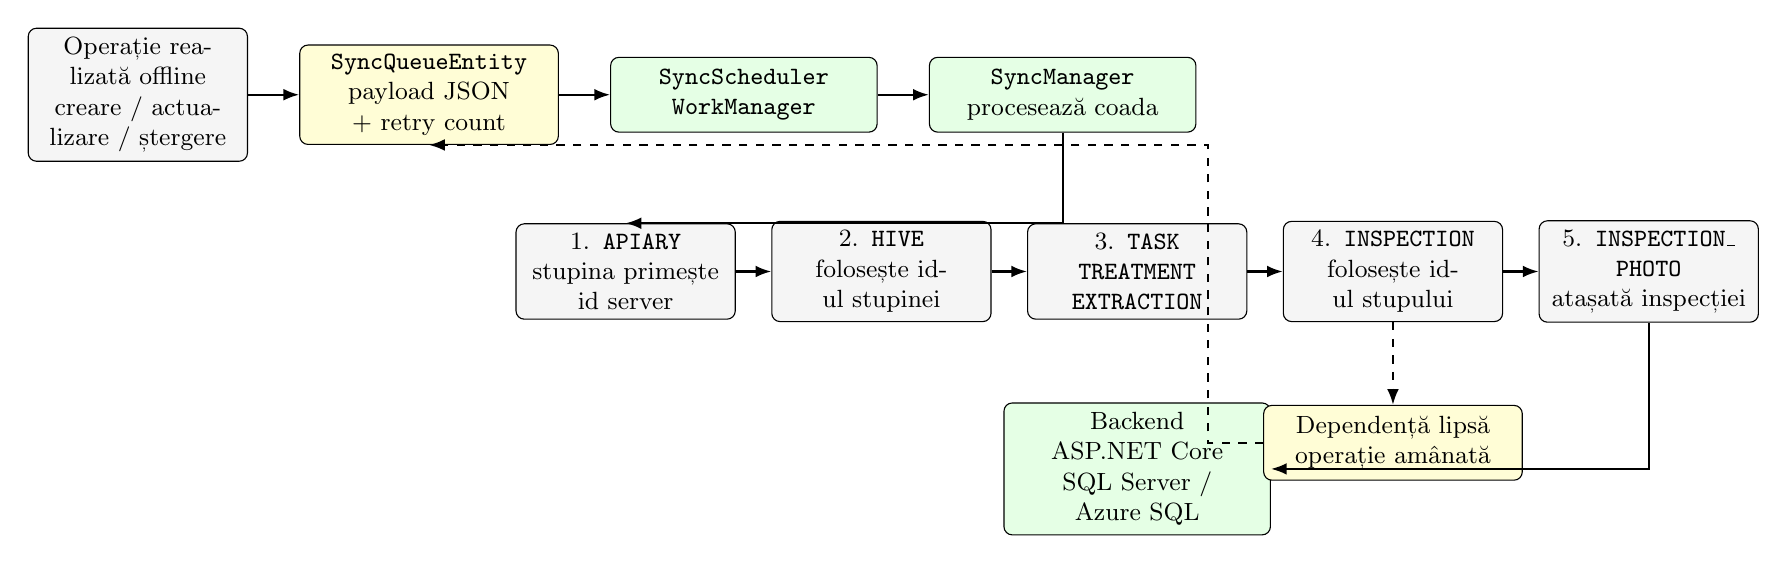
\begin{tikzpicture}[
			syncstep/.style={draw, rounded corners=3pt, fill=gray!8, minimum height=0.95cm, text width=2.55cm, align=center, font=\small},
			queue/.style={draw, rounded corners=3pt, fill=yellow!16, minimum height=0.95cm, text width=3.05cm, align=center, font=\small},
			service/.style={draw, rounded corners=3pt, fill=green!10, minimum height=0.95cm, text width=3.15cm, align=center, font=\small},
			arrow/.style={-{Latex[length=2mm]}, thick},
			defer/.style={-{Latex[length=2mm]}, dashed, thick}
			]
			\node[syncstep] (offline) {Operație realizată offline\\creare / actualizare / ștergere};
			\node[queue, right=0.65cm of offline] (queue) {\texttt{SyncQueueEntity}\\payload JSON + retry count};
			\node[service, right=0.65cm of queue] (scheduler) {\texttt{SyncScheduler}\\\texttt{WorkManager}};
			\node[service, right=0.65cm of scheduler] (manager) {\texttt{SyncManager}\\procesează coada};
			
			\node[syncstep, below=1.15cm of manager, xshift=-5.55cm] (apiary) {1. \texttt{APIARY}\\stupina primește id server};
			\node[syncstep, right=0.45cm of apiary] (hive) {2. \texttt{HIVE}\\folosește id-ul stupinei};
			\node[syncstep, right=0.45cm of hive] (middle) {3. \texttt{TASK}\\\texttt{TREATMENT}\\\texttt{EXTRACTION}};
			\node[syncstep, right=0.45cm of middle] (inspection) {4. \texttt{INSPECTION}\\folosește id-ul stupului};
			\node[syncstep, right=0.45cm of inspection] (photo) {5. \texttt{INSPECTION\_}\\\texttt{PHOTO}\\atașată inspecției};
			
			\node[service, below=1.05cm of middle] (server) {Backend ASP.NET Core\\SQL Server / Azure SQL};
			\node[queue, below=1.05cm of inspection] (deferred) {Dependență lipsă\\operație amânată};
			
			\draw[arrow] (offline) -- (queue);
			\draw[arrow] (queue) -- (scheduler);
			\draw[arrow] (scheduler) -- (manager);
			\draw[arrow] (manager.south) |- (apiary.north);
			\draw[arrow] (apiary) -- (hive);
			\draw[arrow] (hive) -- (middle);
			\draw[arrow] (middle) -- (inspection);
			\draw[arrow] (inspection) -- (photo);
			\draw[arrow] (photo.south) |- (server.east);
			\draw[defer] (inspection) -- (deferred);
			\draw[defer] (deferred.west) -- ++(-0.7,0) |- (queue.south);
	\end{tikzpicture}}
	\caption{Ordinea de execuție a sincronizării offline-first în BeeSmart. Creările sunt trimise în ordinea dependențelor, iar operațiile copil sunt amânate până când părintele primește identificator de server.}
	\label{fig:ordine-sincronizare-offline}
\end{figure}

Ordinea sincronizării este esențială. Codul procesează creările în ordinea: \path{APIARY} \(\rightarrow\) \path{HIVE} \(\rightarrow\) \path{TASK} \(\rightarrow\) \path{TREATMENT} \(\rightarrow\) \path{EXTRACTION} \(\rightarrow\) \path{INSPECTION} \(\rightarrow\) \path{INSPECTION_PHOTO}. Această ordine respectă dependențele dintre entități. Un stup nu poate fi creat pe server înainte ca stupina lui să aibă id de server; o fotografie nu poate fi atașată înainte ca inspecția părinte să existe. Dacă o dependență nu este încă rezolvată, operația este amânată, nu tratată imediat ca eșuată.

Politica de erori diferențiază între probleme de rețea și răspunsuri HTTP invalide. În cazul unor erori de tip \path{IOException}, contorul de reîncercări nu crește, deoarece problema poate fi temporară și independentă de payload. În cazul răspunsurilor HTTP nereușite, contorul crește, iar după trei încercări entitatea poate fi marcată ca eșuată. Această distincție este importantă pentru aplicații mobile, unde lipsa semnalului nu trebuie interpretată automat ca eroare de date.

\section{ASP.NET Core 8 și arhitectura backend}

Backend-ul este implementat în ASP.NET Core 8, framework Microsoft pentru aplicații web și API-uri \cite{aspnetCoreDocs}. ASP.NET Core este potrivit pentru BeeSmart deoarece oferă suport integrat pentru controllere, dependency injection, middleware, autentificare, configurare, logging și integrare cu Entity Framework Core. În proiect, backend-ul este organizat pe straturi: API, Application, Domain și Infrastructure.

Stratul API conține controllerele REST. Acestea primesc cereri HTTP, validează modelul de intrare și apelează serviciile. Stratul Application conține DTO-uri, interfețe, opțiuni și excepții. Stratul Domain conține entitățile de business, iar Infrastructure include \path{AppDbContext}, repository-urile, serviciile concrete, logica de email, JWT și integrarea cu serviciul AI.

Această organizare reduce cuplarea dintre transportul HTTP și logica de domeniu. De exemplu, un controller de inspecții nu ar trebui să știe detalii despre modul în care Entity Framework Core salvează o analiză AI. El primește cererea, extrage utilizatorul din token și pasează operația către serviciu. Serviciul verifică ownership-ul, normalizează datele și folosește repository-ul potrivit.

\section{Entity Framework Core și SQL Server}

Persistența pe server este realizată prin Entity Framework Core, ORM-ul Microsoft pentru .NET \cite{efCoreDocs}. EF Core permite definirea entităților C\# și maparea lor la tabele SQL. În BeeSmart, \path{AppDbContext} definește seturi pentru utilizatori, token-uri, stupine, stupi, task-uri, inspecții, fotografii, analize AI, tratamente și extracții.

Baza de date folosită este SQL Server \cite{sqlServerDocs}, pornită prin Docker Compose pe baza imaginii oficiale Microsoft SQL Server 2022. Pe această variantă a fost realizată proiectarea inițială a schemei și a migrațiilor. Ulterior, pentru găzduirea publică a aplicației, am migrat persistența la Azure SQL Database, serviciul gestionat Microsoft compatibil binar cu SQL Server \cite{azureSqlDocs}. Această compatibilitate a fost o decizie de proiectare deliberată: același set de migrații Entity Framework Core și aceeași definiție a entităților funcționează în ambele variante, fără modificări la nivelul stratului de domeniu.

Relațiile dintre entități sunt configurate explicit în \path{OnModelCreating}. De exemplu, un utilizator are stupine, o stupină are stupi, un stup are inspecții, tratamente și extracții, iar o inspecție poate avea fotografii și analize AI. Pentru unele relații, precum task-urile legate opțional de stupină sau stup, am ales \path{DeleteBehavior.NoAction}, pentru a evita conflictele de cascade.

Entity Framework Core este util și pentru migrații. În \path{Program.cs}, backend-ul aplică migrațiile la pornire, cu retry-uri în cazul în care baza de date nu este încă disponibilă. Această logică se potrivește cu Docker Compose, unde API-ul și SQL Server pornesc ca servicii separate, iar serverul de bază de date poate avea nevoie de câteva secunde pentru inițializare.

\section{Swagger/OpenAPI și documentarea API-ului}

API-ul backend este documentat prin Swagger/OpenAPI. OpenAPI oferă un format standard pentru descrierea endpoint-urilor, parametrilor, răspunsurilor și schemelor folosite de un API REST \cite{swaggerSpec}. În BeeSmart, Swagger este configurat în \path{Program.cs} și include o schemă de securitate Bearer pentru JWT.

În etapa de dezvoltare a BeeSmart, Swagger a fost util pentru testarea endpoint-urilor independent de clientul Android. Interfața generată automat a permis verificarea rapidă a contractelor pentru autentificare, stupine, stupi și inspecții, iar documentarea consecventă a redus riscul ca API-ul să fie consumat în mod greșit de aplicația mobilă.

Pentru a evita expunerea publică a documentației interactive, am configurat activarea interfeței Swagger doar în mediul de dezvoltare. Această alegere păstrează beneficiile documentației la îndemâna echipei, fără a oferi unui consumator extern detalii despre structura internă a API-ului.

\section{Docker Compose și rularea locală}

Docker Compose este folosit pentru pornirea backend-ului, a bazei de date și a serviciului AI ca un ansamblu de containere \cite{dockerComposeDocs}. Fișierul \path{docker-compose.yml} definește trei servicii: \path{sqlserver}, \path{ai-service} și \path{apiaryserver}. Serviciul API depinde de SQL Server și de serviciul AI, iar variabilele de mediu configurează conexiunea la baza de date și URL-ul intern al serviciului AI.

Această configurație simplifică pornirea ansamblului. În loc ca SQL Server, Python, Flask și toate dependențele să fie instalate manual, Docker Compose pornește componentele într-un mod repetabil, pe baza acelorași imagini și a acelorași variabile de mediu. Astfel, fluxul complet poate fi exersat în mod consistent: aplicația Android apelează backend-ul, backend-ul persistă datele și trimite imaginea către serviciul AI pentru detecția și clasificarea celulelor.

\section{Azure Container Apps}

În aplicația Android, URL-ul de bază al API-ului este configurat către endpoint-ul public al backend-ului găzduit în Azure Container Apps. Fișierul \path{NetworkConfig.kt} păstrează această adresă ca valoare de configurare a clientului, destinată exclusiv backend-ului BeeSmart. Aplicația Android nu apelează direct serviciul AI, ci comunică numai cu API-ul, care la rândul lui apelează intern serviciul AI. Această separare păstrează un singur punct public de contact și simplifică gestionarea autentificării, a rate limiting-ului și a verificărilor de ownership.

Azure Container Apps este o platformă serverless pentru aplicații containerizate, cu suport pentru expunerea endpoint-urilor, microservicii, ingress HTTPS, scalare și gestionarea reviziilor \cite{azureContainerAppsDocs}. Pentru BeeSmart, această tehnologie s-a potrivit deoarece atât backend-ul ASP.NET Core, cât și serviciul AI Python sunt construite ca imagini Docker, iar promovarea lor către cloud nu a necesitat rescrieri de cod. În configurația adoptată, API-ul este expus public prin Azure Container Apps, iar serviciul AI rămâne accesibil doar intern, prin rețeaua internă a mediului.

În deployment-ul actual, serviciul AI rulează cu cel puțin o replică activă pentru a evita timpul de pornire al modelelor DeepBee la prima cerere. După testarea pe telefon fizic, containerul AI a fost configurat cu 2 CPU și 4 GiB RAM, iar scalarea este permisă până la trei replici. Backend-ul folosește un timeout de 180 de secunde pentru cererile AI, deoarece analiza unei rame poate include mii de celule detectate și clasificate.

Parametrii importanți ai serviciului AI sunt controlați prin variabile de mediu: \path{DEEPBEE_SEGMENTATION_MAX_SIDE}, \path{DEEPBEE_SEGMENTATION_BATCH_SIZE} și \path{DEEPBEE_CLASSIFICATION_BATCH_SIZE}. Această configurare permite ajustarea consumului de memorie și a timpului de procesare fără schimbarea codului aplicației.

Pe partea de persistență, deploy-ul în Azure a fost completat prin migrarea bazei de date de la SQL Server local către Azure SQL Database \cite{azureSqlDocs}. Astfel, infrastructura de producție a aplicației este unificată în jurul ecosistemului Azure: containerul backend-ului comunică cu instanța gestionată a bazei de date prin string de conexiune dedicat, iar aplicația Android consumă un singur endpoint HTTPS pentru toate fluxurile. Mediul local de dezvoltare păstrează în continuare SQL Server în Docker, ceea ce a permis testarea rapidă a migrațiilor Entity Framework Core și a logicii de acces la date înainte de promovarea modificărilor către instanța din cloud.

Găzduirea publică a backend-ului a fost relevantă și pentru validarea aplicației pe dispozitive reale. Clientul Android a putut fi testat pe telefon, în afara rețelei locale, ceea ce a simplificat verificarea fluxurilor de scanare QR, încărcare de fotografii, autentificare și sincronizare.

\section{Configurarea și gestionarea secretelor}

O aplicație full-stack necesită o gestionare disciplinată a parametrilor de configurare și a secretelor, indiferent de mediul în care rulează. În BeeSmart am separat aceste valori de codul sursă și le-am organizat în surse de configurare dedicate. Cheia OpenWeatherMap este citită din \path{local.properties}, fișier ignorat de Git, astfel încât să nu fie inclusă în istoricul versiunilor. Parola bazei de date este injectată în Docker Compose prin variabila \path{DB_PASSWORD}, iar pe partea de cloud este preluată din configurația mediului Azure. Pe backend, secretul JWT este verificat la pornire: aplicația refuză să pornească dacă valoarea lipsește sau este sub pragul de lungime impus.

Această abordare separă două categorii de parametri. Pe de o parte, valorile publice — precum URL-ul backend-ului expus prin Azure Container Apps — sunt incluse direct în configurația aplicației Android, deoarece reprezintă informație destinată consumului public. Pe de altă parte, secretele propriu-zise — parole, chei API, secret JWT — sunt accesate exclusiv prin variabile de mediu sau prin fișiere ignorate de Git, astfel încât rotația și restricționarea lor să poată fi realizate fără modificări de cod.

\section{OpenWeatherMap și date contextuale}

BeeSmart integrează date meteo prin OpenWeatherMap \cite{openWeatherDocs}. Pe Android, cheia API este citită din \path{local.properties}, astfel încât să nu fie introdusă în repository. \path{WeatherRepository} folosește geocodare, vreme curentă, prognoză și date despre poluarea aerului. Rezultatele de geocodare sunt cache-uite, iar răspunsurile meteo au un TTL de 30 de minute.

Pentru apicultură, vremea este relevantă deoarece activitatea albinelor depinde de temperatură, vânt, precipitații și condiții de zbor. În BeeSmart există și un \path{BeeFlightAdvisor}, care transformă datele brute meteo într-o evaluare simplificată a condițiilor de zbor. Această funcție nu este un model științific complex, dar adaugă context util în interfață.

Integrarea OpenWeatherMap este un exemplu de serviciu extern care nu trebuie să afecteze backend-ul principal. De aceea, aplicația folosește un client Retrofit separat pentru vreme. Dacă API-ul meteo este indisponibil, aplicația poate afișa o stare de indisponibilitate fără să blocheze fluxurile de management apicol.

\section{CameraX, ML Kit Barcode Scanning și ZXing}

Aplicația include funcții de QR și deep link. CameraX este folosit pentru acces modern la camera dispozitivului \cite{cameraXDocs}. ML Kit Barcode Scanning permite detectarea codurilor QR din fluxul camerei \cite{mlkitBarcodeDocs}, iar ZXing este folosit pentru generarea codurilor QR \cite{zxingProject}. În BeeSmart, fiecare stup poate fi asociat cu un link de tip deep link, iar codul QR poate fi scanat pentru deschiderea rapidă a fișei stupului.

Această funcționalitate este potrivită pentru teren. În loc ca apicultorul să caute manual un stup în listă, poate scana codul atașat fizic pe stup. Deep link-ul poate folosi schema proprie \path{beesmart://} sau schema HTTPS configurată prin variabile Gradle. În proiect, gazda implicită este \path{app.beesmart.ro}, iar adresele pentru stupi pot avea forma \path{/hive/{hiveId}}.

Din punct de vedere tehnic, folosirea CameraX și ML Kit separă două responsabilități. CameraX se ocupă de captarea imaginii, iar ML Kit interpretează conținutul vizual pentru a detecta codul. ZXing completează fluxul invers, generând codul care va fi imprimat sau salvat.

\section{Recunoaștere vocală}

BeeSmart include și un mecanism de introducere vocală a datelor, încapsulat în \path{VoiceCommandManager}. Acesta folosește API-ul Android \path{SpeechRecognizer}, care permite aplicațiilor să trimită audio către un serviciu de recunoaștere disponibil pe dispozitiv \cite{androidSpeechRecognizerDocs}. Limba implicită este româna, configurată prin \path{ro-RO}, iar rezultatele sunt transmise către ViewModel printr-un \path{Flow}.

După recunoaștere, textul este procesat prin reguli simple pentru completarea unor câmpuri. De exemplu, expresii precum \enquote{numele este}, \enquote{locația este}, \enquote{temperatura este} sau \enquote{rame cu puiet} sunt asociate unor câmpuri din formular. Această abordare nu este un sistem NLP complex, dar este suficientă pentru comenzi scurte de teren. Ea poate reduce timpul de introducere a datelor atunci când utilizatorul nu vrea să tasteze.

Funcția se bazează exclusiv pe API-ul de recunoaștere vocală oferit de platforma Android, nu pe un serviciu propriu de procesare a limbajului natural. Prin urmare, introducerea vocală reprezintă o îmbunătățire de ergonomie a interfeței, nu o componentă AI dezvoltată în cadrul proiectului.

\section{Serviciul AI: Flask, OpenCV, TensorFlow și Keras}

Serviciul AI este implementat în Python și se află în directorul \path{ApiaryServer/ApiaryServer/AIService}. El folosește Flask pentru expunerea endpoint-urilor HTTP \path{/analyze} și \path{/health} \cite{flaskDocs}, OpenCV pentru procesarea imaginilor \cite{opencvDocs}, TensorFlow și Keras pentru încărcarea modelelor DeepBee \cite{tensorflowDocs,kerasDocs}. Modelele folosite sunt \path{classification.h5} și \path{segmentation.h5}, provenite din articolul DeepBee \cite{deepbeeArticle} și din implementarea de referință disponibilă public \cite{deepbeeSource}. Fișierul \path{requirements.txt} indică versiuni specifice, printre care TensorFlow 1.14.0 și Keras 2.2.4.

Fluxul serviciului este următorul. Backend-ul trimite o imagine Base64. Serviciul decodează imaginea, verifică dacă payload-ul este valid, calculează metrici de calitate și respinge fotografiile prea mici, prea neclare, prea întunecate, supraexpuse sau cu contrast insuficient. Dacă imaginea trece aceste verificări, serviciul aplică segmentarea semantică, detectează celulele prin Hough Circle Transform pe canalul roșu, extrage regiuni proporționale cu raza celulei, le redimensionează la 224 x 224 pixeli și le preprocesează cu \path{preprocess_input}. Clasificarea este executată în loturi, pentru ca serviciul să nu încarce simultan în memorie toate crop-urile rezultate dintr-o ramă densă.

Ordinea claselor interpretate din modelul de clasificare este \path{Capped}, \path{Eggs}, \path{Honey}, \path{Larves}, \path{Nectar}, \path{Other} și \path{Pollen}. Această ordine este preluată din repository-ul DeepBee și este esențială deoarece ieșirea modelului este un vector numeric de probabilități. Rezultatul serviciului conține numărul de celule pe fiecare clasă, un status și metadate de calitate. Statusul poate indica succes, imagine de calitate scăzută, imagine care nu pare fagure sau analiză incertă. Această logică este importantă deoarece un model AI nu trebuie forțat să ofere un rezultat aparent precis pentru o imagine nepotrivită.

În backend, \path{AiAnalysisService} trimite imaginea către serviciul Python prin \path{HttpClient}. Endpoint-ul \path{POST inspections/analyze-cells} validează Base64-ul, păstrează metadatele \path{quality} returnate de AI și tratează erorile de serviciu prin răspunsuri HTTP precum 502 sau 504. Astfel, clientul Android primește un răspuns controlat, nu o eroare brută de infrastructură.

\section{Tehnologii de testare}

Partea Android include teste JVM cu JUnit, Robolectric, Room in-memory și MockWebServer. Robolectric permite rularea unor teste Android pe JVM, fără emulator, și poate include resurse Android în testele unitare \cite{robolectricDocs}. MockWebServer permite simularea răspunsurilor HTTP, ceea ce este util pentru verificarea repository-urilor și a sincronizării fără dependență de un server real.

În proiect există un \path{SyncTestHarness}, care leagă o bază Room in-memory, un client Retrofit real și un server mock. Această infrastructură testează scenarii offline-online: se setează aplicația offline, se creează entități locale, apoi se reactivează conexiunea, se pun răspunsuri mock și se rulează \path{SyncManager}. Testele verifică atât cererile HTTP primite de serverul mock, cât și starea bazei locale și golirea cozii.

Backend-ul are un proiect separat de teste xUnit. Testele acoperă servicii precum \path{ApiaryService} și \path{AiAnalysisService}, inclusiv cazuri de ownership, mapare a datelor și tratare a erorilor de la serviciul AI.
\section{Observații privind alegerea tehnologiilor}

Stiva tehnologică BeeSmart este coerentă cu tipul aplicației. Kotlin, Compose, Room și WorkManager susțin partea mobilă offline-first. Retrofit, OkHttp și Moshi oferă comunicarea cu backend-ul. ASP.NET Core și Entity Framework Core susțin un API robust, persistent inițial pe SQL Server și migrat ulterior pe Azure SQL Database pentru varianta publică. Docker Compose asigură un mediu local reproductibil, iar Azure Container Apps găzduiește backend-ul accesibil utilizatorilor. Flask, OpenCV, TensorFlow și Keras permit separarea analizei AI într-un serviciu specializat.

În același timp, tehnologiile nu sunt suficiente prin simpla lor prezență. Valoarea proiectului apare din modul în care sunt conectate: repository-urile decid între rețea și Room, coada de sincronizare păstrează operațiile offline, backend-ul verifică ownership-ul, iar serviciul AI este apelat prin API, nu direct din aplicația mobilă. Această integrare va fi susținută în capitolul teoretic prin concepte precum trasabilitate, offline-first, consistență eventuală, clasificarea imaginilor și responsabilitatea interpretării rezultatelor AI.

\chapter{Suport teoretic}
\label{chap:suport-teoretic}

\section{Apicultură digitală și trasabilitatea lucrărilor}

Digitalizarea apiculturii se înscrie într-o direcție mai amplă, cunoscută în literatura de specialitate sub numele de \emph{apicultură de precizie} (\emph{Precision Beekeeping}), care urmărește gestionarea fiecărei familii de albine pe baza datelor colectate, pentru a reduce pierderile și a îmbunătăți deciziile apicultorului \cite{zacepins2015precision}. Lucrările din acest domeniu arată că monitorizarea continuă și înregistrarea sistematică a stării coloniilor oferă informații utile pentru intervenții la timp \cite{meikle2015monitoring}. Totuși, digitalizarea apiculturii nu înseamnă doar mutarea unei agende pe telefon. O aplicație utilă trebuie să transforme observațiile de teren în date care pot fi regăsite, comparate și interpretate. În apicultură, aceeași familie de albine trece prin stări diferite de-a lungul sezonului: dezvoltare de primăvară, cules, roire, tratamente, pregătire pentru iernare și perioade de repaus. Pentru a înțelege corect starea unui stup, apicultorul are nevoie de continuitate între observații.

Conceptul de trasabilitate este relevant în acest context. Trasabilitatea presupune păstrarea unui istoric coerent al evenimentelor care afectează un obiect urmărit. În BeeSmart, obiectul urmărit poate fi stupina, stupul sau inspecția. Pentru un stup, istoricul poate include date despre matcă, rame, puiet, rezerve, tratamente, extracții, fotografii și analize AI. Dacă aceste informații sunt introduse consecvent, aplicația poate oferi o imagine mai clară decât o notă izolată.

Trasabilitatea este importantă și pentru decizii practice. De exemplu, un tratament antivarroa trebuie urmărit în timp, nu doar notat în ziua aplicării. O scădere a puietului trebuie comparată cu inspecțiile anterioare, nu interpretată fără context. O extracție trebuie corelată cu perioada de cules și cu starea familiei. În lipsa unui sistem digital, aceste corelații depind de memoria utilizatorului sau de calitatea agendei scrise.

BeeSmart urmărește să ofere această structură prin entități clare: stupine, stupi, inspecții, tratamente, extracții și task-uri. Fiecare entitate contribuie la istoricul apicol.

\section{Datele apicole ca date sezoniere}

Un aspect specific apiculturii este sezonalitatea. Datele apicole nu sunt uniforme pe tot parcursul anului. Primăvara, accentul cade pe dezvoltarea familiei, existența mătcii și extinderea cuibului. Vara, atenția se mută spre cules, spațiu, prevenirea roirii și extracții. Toamna, tratamentele și pregătirea rezervelor devin prioritare. Iarna, activitatea de inspecție este redusă, dar istoricul rămâne util pentru planificarea sezonului următor.

Din perspectiva unei aplicații, această sezonalitate înseamnă că datele trebuie păstrate în timp și prezentate comparativ. O valoare precum numărul de rame cu puiet este utilă doar dacă poate fi raportată la data inspecției și la starea anterioară a stupului. De aceea, BeeSmart nu se limitează la o listă curentă de stupi. Aplicația păstrează istoricul inspecțiilor și poate folosi rezultatele AI pentru a construi tendințe.

Un alt efect al sezonalității este faptul că anumite date sunt importante doar în contexte precise. Vremea contează în mod special la inspecții, zbor și cules. Tratamentele au ferestre de aplicare. Extracțiile sunt relevante în raport cu culesul și cu rezervele rămase în stup. Task-urile ajută la planificarea acestor intervenții, dar ele trebuie legate de stupină sau stup pentru a nu deveni simple memento-uri generale.

\section{Inspecția ca act central în managementul apicol}

Inspecția este una dintre operațiile centrale ale managementului apicol. În timpul unei inspecții, apicultorul observă direct starea familiei și notează informații despre cuib, hrană, matcă, puiet și eventuale probleme. În BeeSmart, formularul de inspecție reflectă aceste elemente prin câmpuri precum temperatura, numărul total de rame, rame cu puiet, rame cu miere, rame cu polen, prezența mătcii, prezența ouălor și a larvelor.

O inspecție are valoare imediată, dar și valoare istorică. Valoarea imediată apare în decizia de moment: trebuie adăugată hrană, trebuie căutată matca, trebuie verificată roirea, trebuie aplicat tratament. Valoarea istorică apare când inspecția este comparată cu altele. Dacă un stup avea puiet compact la începutul lunii și apoi scade brusc, aplicația poate ajuta utilizatorul să observe schimbarea. Dacă tratamentele și extracțiile sunt păstrate în același sistem, datele devin mai ușor de corelat.

În proiectarea unei aplicații mobile, formularul de inspecție trebuie să fie suficient de detaliat, dar nu excesiv de încărcat. Dacă formularul este prea simplu, nu colectează date utile. Dacă este prea lung, utilizatorul nu îl va completa în teren. BeeSmart încearcă să echilibreze aceste cerințe prin câmpuri structurate, fotografii, introducere vocală și valori care pot fi completate rapid.

\section{Rolul fotografiilor de rame}

Fotografia unei rame adaugă un strat vizual la inspecție. Ea poate surprinde detalii pe care utilizatorul nu le notează complet în momentul inspecției. Poate fi revăzută ulterior, comparată cu alte imagini și folosită pentru analiză automată. În aplicații apicole, fotografia nu trebuie privită doar ca atașament decorativ, ci ca o formă de date.

Totuși, o fotografie brută are limite. Două imagini pot fi greu de comparat dacă sunt făcute la distanțe diferite, în lumină diferită sau din unghiuri diferite. De aceea, analiza automată urmărește să transforme imaginea într-o reprezentare numerică: câte celule au fost detectate, câte aparțin fiecărei clase și ce indicatori pot fi calculați din aceste valori.

În BeeSmart, fotografia este introdusă din formularul de inspecție și este trimisă către backend pentru analiză. Clientul Android nu rulează modelul DeepBee direct. Această decizie are avantajul de a păstra aplicația mobilă mai ușoară și de a centraliza procesarea AI într-un serviciu specializat. Dezavantajul este că analiza necesită conexiune la backend și la serviciul AI. Prin urmare, fotografia poate exista ca parte a inspecției offline, dar analiza automată depinde de infrastructura server.

În implementarea curentă, fotografia are două reprezentări practice. Prima este fișierul procesat păstrat pentru inspecție, la o calitate potrivită pentru arhivare și revizualizare. A doua este versiunea trimisă către AI, redimensionată la maximum 1536 px și comprimată înainte de codarea Base64. Această separare a redus payload-ul transmis de pe telefon, fără să elimine fotografia din istoricul inspecției.

\section{Sisteme offline-first}

Un sistem offline-first este proiectat astfel încât absența temporară a conexiunii să nu blocheze complet utilizarea aplicației. Într-un model clasic, clientul trimite cereri la server și așteaptă răspunsul pentru a considera operația finalizată. Într-un model offline-first, clientul păstrează o copie locală a datelor și poate înregistra operații care vor fi sincronizate ulterior.

Pentru BeeSmart, această strategie este justificată de mediul de utilizare. Stupinele pot fi amplasate în zone cu semnal slab, iar apicultorul nu ar trebui să piardă date doar pentru că serverul nu este accesibil în acel moment. Când utilizatorul creează o inspecție offline, aplicația trebuie să îi ofere un răspuns imediat și să salveze local operația. Când conexiunea revine, aplicația trimite datele la server.

Din punct de vedere teoretic, offline-first introduce problema consistenței. Datele locale pot fi temporar diferite de cele de pe server. Această stare este acceptabilă dacă aplicația știe ce operații sunt în așteptare și le poate sincroniza într-o ordine corectă. În BeeSmart, coada de sincronizare este soluția pentru această problemă. Ea reține operațiile și permite procesarea lor când condițiile de rețea sunt favorabile.

\section{Consistență eventuală și dependențe între entități}

Consistența eventuală înseamnă că sistemul poate avea stări temporar diferite în componente diferite, dar urmărește ca acestea să ajungă la aceeași stare după sincronizare \cite{vogelsEventualConsistency}. Într-o aplicație mobilă offline, această idee apare natural. Telefonul poate conține date noi pe care serverul nu le-a primit încă. După sincronizare, serverul primește datele, iar clientul actualizează identificatorii și statusurile locale.

În BeeSmart, dependențele dintre entități fac sincronizarea mai complexă. O stupină poate exista fără stupi, dar un stup are nevoie de o stupină. O inspecție are nevoie de un stup. O fotografie are nevoie de o inspecție. Dacă utilizatorul creează offline toate aceste elemente, aplicația trebuie să păstreze relațiile locale și apoi să le transforme în relații de server. Aceasta este problema rezolvării identificatorilor.

De exemplu, o stupină creată offline primește un id local. Stupul creat în acea stupină referă id-ul local al stupinei. Când stupina este sincronizată, serverul returnează un id real. Abia apoi stupul poate fi trimis la server cu id-ul corect al stupinei. Același principiu se aplică în lanțul de dependențe prezentat în figura~\ref{fig:ordine-sincronizare-offline}: de la stupină, către stup, apoi către task-uri, tratamente, extracții, inspecții și, în final, fotografii. Dacă aplicația ar încerca să trimită un element copil înainte ca părintele să fie sincronizat, backend-ul nu ar putea găsi referința. De aceea, procesarea în ordinea dependențelor nu este un detaliu de implementare, ci o cerință teoretică a modelului offline-first.

\section{Securitatea datelor și ownership}

BeeSmart gestionează date care aparțin unui utilizator: stupine, stupi, inspecții, fotografii și analize. Chiar dacă aceste date nu sunt la fel de sensibile ca datele medicale sau financiare, ele pot avea valoare economică și profesională. Un apicultor nu ar trebui să poată accesa datele altuia, iar pierderea sau amestecarea datelor ar afecta încrederea în aplicație.

Autentificarea prin JWT rezolvă doar o parte a problemei. Un token valid arată că utilizatorul este autentificat, dar nu demonstrează automat că are dreptul asupra fiecărei resurse cerute. De aceea, backend-ul trebuie să verifice ownership-ul la nivel de servicii și repository-uri. În BeeSmart, controllerele extrag id-ul utilizatorului din token, iar serviciile verifică dacă resursele aparțin acelui utilizator înainte de mutații.

Pe client, securitatea se leagă și de starea locală. Dacă utilizatorul se deloghează sau se autentifică alt cont, aplicația trebuie să evite afișarea datelor vechi. De asemenea, token-urile trebuie gestionate cu atenție, iar refresh-ul nu trebuie să creeze bucle de cereri. Aceste aspecte sunt relevante pentru orice aplicație offline-first, deoarece datele persistă pe dispozitiv chiar și după întreruperi de rețea.

\section{DeepBee ca punct de plecare pentru analiza ramelor}

Componenta teoretică principală a analizei automate este articolul \enquote{Automatic detection and classification of honey bee comb cells using deep learning} \cite{deepbeeArticle}. Articolul prezintă o metodă pentru detectarea și clasificarea celulelor din imagini de fagure. Scopul unei astfel de metode este extragerea automată a unor informații care, altfel, ar necesita observare manuală atentă.

DeepBee împarte problema în mai multe etape. Mai întâi, celulele trebuie detectate în imagine. Apoi, regiunile detectate trebuie filtrate pentru a reduce detecțiile false. În final, fiecare celulă detectată trebuie clasificată într-una dintre clasele relevante. Această împărțire este logică: înainte de a decide ce conține o celulă, sistemul trebuie să știe unde se află celula.

Pentru BeeSmart, articolul DeepBee oferă baza conceptuală pentru integrarea AI. Aplicația nu revendică modelul ca fiind original, ci folosește ideea de analiză automată a celulelor pentru a completa inspecțiile apicole. În acest fel, contribuția lucrării este aplicativă: modelul este introdus într-un flux Android-backend-AI, iar rezultatul devine parte a istoricului stupului.

Integrarea a pornit de la implementarea de referință publicată de autori \cite{deepbeeSource}, iar nucleul algoritmic a fost păstrat fidel: aceleași modele \path{segmentation.h5} și \path{classification.h5}, aceeași ordine a claselor la decodarea predicțiilor, aceiași parametri ai transformatei Hough (inclusiv formula razei dominante pentru distanța minimă dintre centre), aceeași pregătire a imaginii pe canalul roșu cu egalizare locală de contrast și filtrare bilaterală și aceeași decupare proporțională cu raza, redimensionată la 224 x 224 pixeli înainte de clasificare. Fidelitatea față de varianta originală este importantă pentru corectitudine: modelul a fost antrenat pe un anumit mod de pregătire a datelor, iar o abatere de la acesta ar degrada predicțiile fără ca formatul răspunsului să pară greșit.

În același timp, codul de referință este o aplicație desktop care procesează loturi de fotografii din foldere locale și presupune resurse de calcul generoase. Pentru ca metoda să poată fi apelată dintr-o aplicație mobilă, în cadrul lucrării au fost necesare mai multe adaptări:
\begin{itemize}
	\item transformarea pipeline-ului într-un microserviciu Flask cu rutele \path{/analyze} și \path{/health}, cu intrare Base64 și răspuns JSON; inferența folosește o singură sesiune TensorFlow partajată și este serializată printr-un mecanism de blocare, deoarece combinația Keras 2 / TensorFlow 1 nu este thread-safe într-un server web;
	\item înlocuirea reconstrucției măștii de segmentare la rezoluția fixă de 6000 x 4000 pixeli cu o limită configurabilă a muchiei maxime (implicit 2200 px) și cu o grilă de patch-uri calculată dinamic pe dimensiunile reale ale imaginii, masca rezultată fiind scalată înapoi peste imaginea analizată; această schimbare face inferența stabilă pe containerul cu resurse limitate din Azure;
	\item restructurarea clasificării astfel încât decupajele de 224 x 224 pixeli să fie extrase și clasificate în loturi, fără a păstra simultan în memorie toate regiunile unei rame dense, așa cum procedează varianta originală;
	\item reinterpretarea scorului de încredere: în codul original, pragul foarte ridicat de 0,9995 marchează doar celulele potrivite pentru reantrenarea modelului, în timp ce în BeeSmart un prag de 0,60 pe celulă și un raport maxim de 75\% predicții slabe decid dacă întreaga analiză este declarată incertă.
\end{itemize}

Pe lângă aceste adaptări, serviciul adaugă elemente care nu există în implementarea de referință: criteriile de calitate aplicate înainte de model (dimensiune minimă, claritate, luminozitate, contrast), statusurile de răspuns dedicate imaginilor nepotrivite, pragul minim de celule detectate și metadatele de calitate atașate fiecărui răspuns (numărul de celule detectate și clasificate, încrederea medie și timpii pe etape). Aceste extensii sunt detaliate în secțiunile următoare ale capitolului. În sens invers, componentele desktop ale proiectului original — vizualizarea interactivă, corectarea manuală a predicțiilor, exportul tabelar și reantrenarea — nu au fost preluate, deoarece nu se potrivesc unui serviciu apelat automat din aplicație. Ca format de răspuns, serviciul întoarce distribuția celulelor pe clase împreună cu metadatele de calitate, adică exact forma de care au nevoie indicatorii derivați și statisticile longitudinale construite peste analiză în aplicație.

\section{Cele șapte clase de celule}

Modelul DeepBee urmărește clasificarea celulelor în șapte clase: ouă, larve, puiet căpăcit, polen, nectar, miere și alte celule \cite{deepbeeArticle}. Aceste clase sunt relevante deoarece descriu atât activitatea de reproducere a coloniei, cât și rezervele de hrană. Ouăle și larvele indică prezența unei ponte recente, puietul căpăcit indică dezvoltarea în curs, iar mierea, nectarul și polenul descriu resursele disponibile.

În serviciul BeeSmart, ieșirea modelului este interpretată în ordinea folosită de repository-ul DeepBee: \path{Capped}, \path{Eggs}, \path{Honey}, \path{Larves}, \path{Nectar}, \path{Other} și \path{Pollen}. Această ordine este importantă deoarece vectorul de probabilități produs de rețeaua neuronală nu conține etichete text, ci doar poziții numerice. Dacă pozițiile ar fi asociate greșit, rezultatul ar părea valid ca format, dar ar descrie categorii biologice eronate. În interfața pentru utilizator, rezultatele pot fi asociate unor termeni românești, iar în backend sunt normalizate pentru calcule.

Clasa \enquote{alte celule} este importantă deoarece nu toate regiunile detectate pot fi atribuite sigur uneia dintre clasele principale. În practică, pot exista celule goale, celule acoperite parțial, zone neclare sau regiuni detectate greșit. O clasificare responsabilă trebuie să accepte incertitudinea, nu să forțeze fiecare regiune într-o categorie apicolă precisă.

\section{Detecția celulelor cu Hough Circle Transform}

Celulele fagurelui au o formă aproximativ regulată. Într-o fotografie frontală, ele pot fi tratate ca regiuni aproape circulare sau eliptice, deși în realitate geometria fagurelui este hexagonală. Hough Circle Transform este o tehnică de procesare a imaginilor folosită pentru identificarea cercurilor în imagini \cite{opencvDocs}. Ideea generală este că punctele de margine din imagine votează pentru posibile cercuri, iar zonele cu multe voturi indică existența unor forme circulare.

Din punct de vedere matematic, un cerc din planul imaginii este descris de ecuația
\begin{equation}
	(x - a)^2 + (y - b)^2 = r^2,
	\label{eq:cerc}
\end{equation}
unde $(a, b)$ este centrul, iar $r$ raza. Un punct de margine $(x, y)$ detectat în imagine este compatibil cu o întreagă familie de cercuri, parametrizată de tripletul $(a, b, r)$. Transformata Hough mută problema din spațiul imaginii în spațiul parametrilor: fiecare punct de margine votează pentru toate combinațiile $(a, b, r)$ care satisfac relația \eqref{eq:cerc}. Formal, valoarea acumulatorului pentru un candidat $(a, b, r)$ este
\begin{equation}
	H(a, b, r) = \sum_{(x, y) \in E} \mathbf{1}\!\left[\, \bigl| (x - a)^2 + (y - b)^2 - r^2 \bigr| \le \varepsilon \,\right],
	\label{eq:hough-acumulator}
\end{equation}
unde $E$ este mulțimea punctelor de margine, $\mathbf{1}[\cdot]$ este funcția indicator, iar $\varepsilon$ o toleranță care compensează discretizarea și zgomotul. Centrele de celulă reale corespund maximelor locale ale acumulatorului $H$. Pentru a reduce dimensionalitatea problemei, implementarea OpenCV folosește varianta bazată pe gradient (\path{HOUGH_GRADIENT}), în care direcția gradientului din fiecare punct de margine restrânge votul la centre situate de-a lungul normalei locale, în loc să acopere întreg spațiul parametrilor.

Articolul DeepBee folosește această direcție pentru detecția celulelor \cite{deepbeeArticle}. În BeeSmart, serviciul Python pregătește imaginea prin folosirea canalului roșu, egalizare locală de contrast și filtrare bilaterală. Apoi, funcția de detecție rulează o etapă inițială pentru estimarea razei tipice a celulelor și o etapă finală cu parametri adaptați. Această adaptare este necesară deoarece aceeași celulă poate ocupa un număr diferit de pixeli în funcție de distanța camerei, rezoluție și încadrare.

Detecția nu garantează perfectitudinea. Pot apărea detecții lipsă sau detecții false. Zonele cu reflexii, umbre, ceară neregulată sau celule parțial vizibile pot influența rezultatul. De aceea, detecția trebuie privită ca etapă inițială, nu ca rezultat final. În BeeSmart, după detecție urmează clasificarea regiunilor și verificări de calitate.

\section{Segmentarea semantică și eliminarea detecțiilor false}

În teoria modelului DeepBee, segmentarea semantică este folosită pentru a reduce detecțiile false \cite{deepbeeArticle}. Segmentarea semantică înseamnă atribuirea unei clase fiecărui pixel sau fiecărei regiuni, pentru a separa zonele relevante de fundal. În cazul imaginilor de rame, această etapă poate ajuta la eliminarea cercurilor detectate în zone care nu reprezintă celule reale.

În implementarea BeeSmart, serviciul AI folosește modelul \path{segmentation.h5} din repository-ul DeepBee pentru a separa zona relevantă a ramei de fundal. Masca obținută este folosită pentru a calcula regiunea de interes și pentru a elimina cercurile detectate în afara fagurelui. După această etapă, detecția celulelor se face prin Hough Circle Transform pe canalul roșu, cu egalizare locală de contrast și filtrare bilaterală, urmând logica pipeline-ului DeepBee.

Față de varianta experimentală DeepBee, care reconstruiește masca la o rezoluție fixă mare, integrarea BeeSmart folosește o limită configurabilă a muchiei maxime. În deployment-ul curent, segmentarea este limitată la 2200 px, iar imaginea este împărțită în patch-uri procesate în loturi. Masca este apoi scalată peste imaginea analizată. Această adaptare păstrează rolul semantic al segmentării, dar reduce memoria necesară și face inferența mai stabilă în container.

Pe lângă segmentare, BeeSmart include filtre practice de calitate: dimensiune minimă a imaginii, claritate, luminozitate, contrast, număr minim de celule detectate și raport al predicțiilor cu încredere scăzută. Dacă imaginea nu trece aceste criterii, serviciul întoarce un status precum \path{low_quality}, \path{not_comb_image} sau \path{uncertain_analysis}. În acest mod, aplicația combină pipeline-ul original DeepBee cu validări orientate spre utilizarea în teren.

\section{Rețele neuronale convoluționale}

Clasificarea imaginilor se bazează frecvent pe rețele neuronale convoluționale, care reprezintă astăzi abordarea dominantă în recunoașterea automată a imaginilor \cite{lecun2015deeplearning}. Adoptarea lor pe scară largă a fost accelerată de rezultatele obținute pe seturi mari de date precum ImageNet, unde rețelele convoluționale profunde au depășit semnificativ metodele clasice de extragere manuală a caracteristicilor \cite{krizhevsky2012imagenet}. O rețea convoluțională folosește filtre care extrag tipare locale din imagine: margini, texturi, forme și combinații tot mai complexe de caracteristici. În straturile inițiale, rețeaua poate învăța forme simple; în straturile profunde, poate învăța reprezentări mai abstracte \cite{Goodfellow-et-al-2016}.

Operația fundamentală a acestor rețele este convoluția discretă. Pentru o intrare $I$ și un nucleu (filtru) $K$ de dimensiune $m \times n$, harta de caracteristici rezultată într-o poziție $(i, j)$ se calculează ca
\begin{equation}
	S(i, j) = (I * K)(i, j) = \sum_{u=0}^{m-1} \sum_{v=0}^{n-1} I(i + u, \, j + v)\, K(u, v) + b,
	\label{eq:convolutie}
\end{equation}
unde $b$ este termenul de bias. Asupra rezultatului se aplică o funcție de activare neliniară, de regulă ReLU, $\sigma(z) = \max(0, z)$, care introduce neliniaritatea necesară învățării de reprezentări complexe. Straturile de pooling reduc apoi rezoluția spațială, păstrând informația dominantă și scăzând costul de calcul.

Pentru clasificarea celulelor din fagure, o rețea convoluțională primește o regiune de imagine și produce un vector de scoruri $\mathbf{z} = (z_1, \dots, z_C)$, câte unul pentru fiecare dintre cele $C$ clase. Acest vector este transformat în probabilități prin funcția softmax:
\begin{equation}
	p_k = \frac{e^{z_k}}{\sum_{c=1}^{C} e^{z_c}}, \qquad k = 1, \dots, C,
	\label{eq:softmax}
\end{equation}
care garantează $p_k \in (0, 1)$ și $\sum_{c=1}^{C} p_c = 1$. Clasa atribuită celulei este cea cu probabilitatea maximă, $\hat{y} = \arg\max_k p_k$, iar valoarea $\max_k p_k$ reprezintă încrederea predicției.

În BeeSmart, fiecare celulă detectată este extrasă proporțional cu raza estimată, redimensionată la $224 \times 224$ pixeli, preprocesată conform funcției \path{preprocess_input} din Keras și trimisă modelului. Modelul întoarce scorurile din relația \eqref{eq:softmax}, iar clasa cu probabilitatea cea mai mare este folosită pentru numărătoare. Încrederea predicției este păstrată ca metadată de calitate și poate transforma rezultatul într-o analiză incertă dacă prea multe celule au $\max_k p_k$ sub un prag stabilit.

\begin{figure}[H]
	\centering
	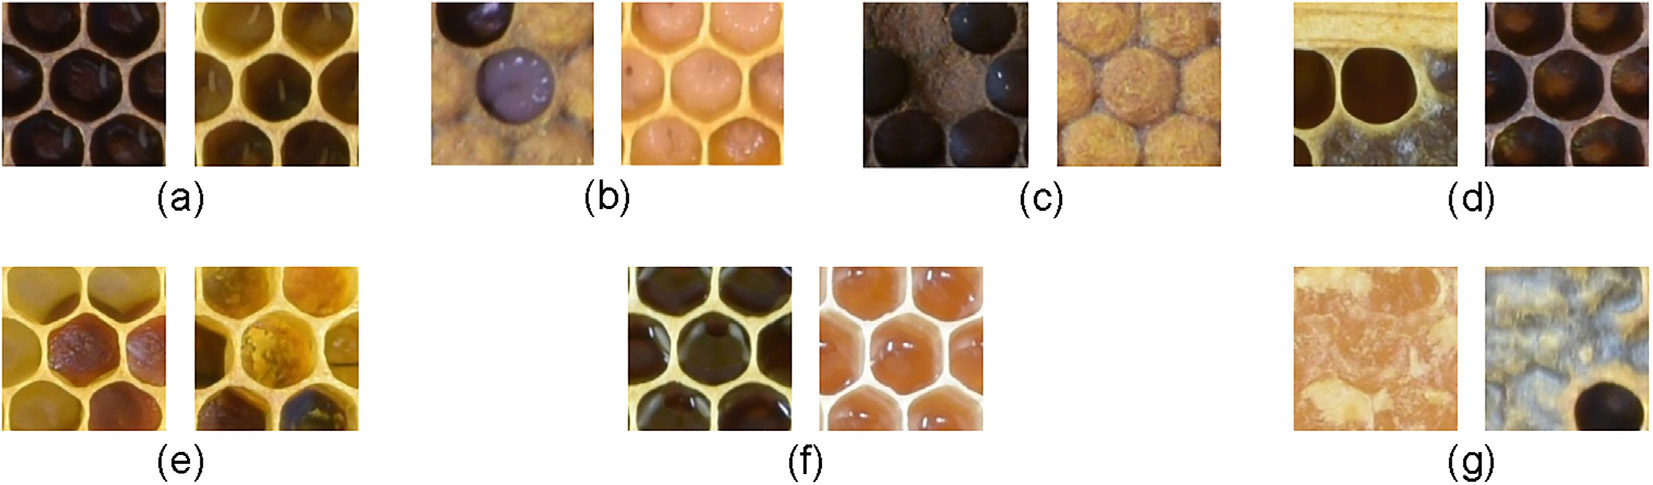
\includegraphics[width=\textwidth]{./images/deepbee-cell-classes.jpg}
	\caption{Exemple vizuale de clase de celule de fagure folosite în articolul DeepBee pentru clasificarea automată. Imagine preluată din articolul \cite{deepbeeArticle}.}
	\label{fig:deepbee-clase-celule}
\end{figure}

Pornind de la aceste exemple vizuale (figura~\ref{fig:deepbee-clase-celule}), fluxul conceptual al clasificării poate fi rezumat printr-o succesiune de pași: pregătirea regiunii de imagine, extragerea caracteristicilor prin straturi convoluționale și transformarea rezultatului în probabilități pentru clasele relevante. Acest flux este ilustrat în figura~\ref{fig:flux-cnn-celule-fagure}.

\begin{figure}[H]
	\centering
	\resizebox{\textwidth}{!}{%
	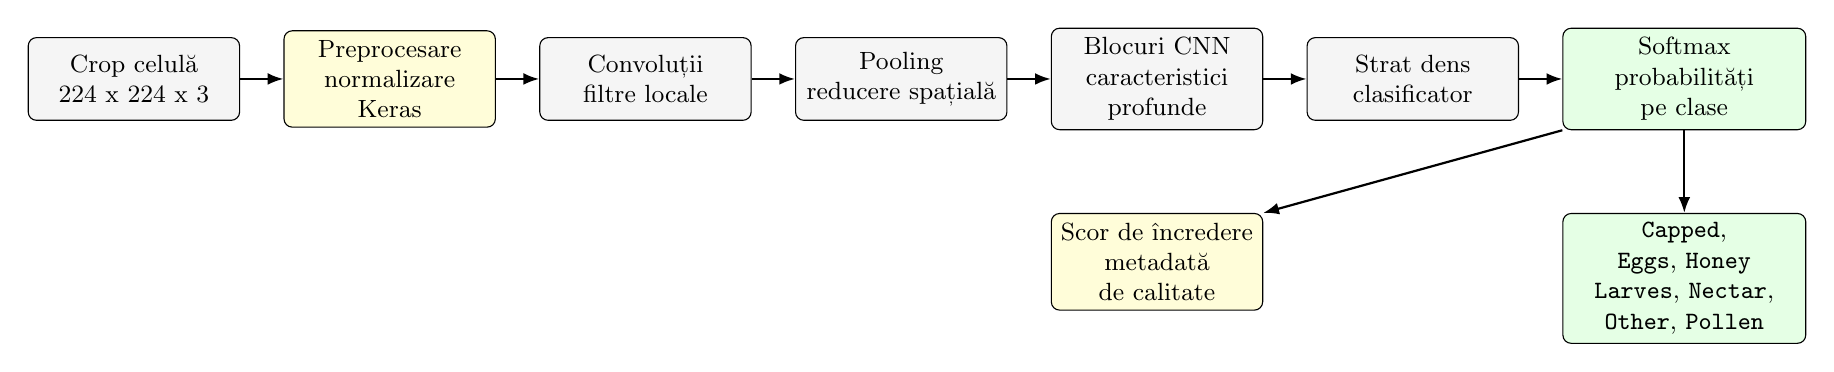
\begin{tikzpicture}[
		layer/.style={draw, rounded corners=3pt, fill=gray!8, minimum height=1.05cm, text width=2.45cm, align=center, font=\small},
		process/.style={draw, rounded corners=3pt, fill=yellow!15, minimum height=1.05cm, text width=2.45cm, align=center, font=\small},
		output/.style={draw, rounded corners=3pt, fill=green!10, minimum height=1.05cm, text width=2.85cm, align=center, font=\small},
		arrow/.style={-{Latex[length=2mm]}, thick}
	]
		\node[layer] (input) {Crop celulă\\224 x 224 x 3};
		\node[process, right=0.55cm of input] (prep) {Preprocesare\\normalizare Keras};
		\node[layer, right=0.55cm of prep] (conv1) {Convoluții\\filtre locale};
		\node[layer, right=0.55cm of conv1] (pool1) {Pooling\\reducere spațială};
		\node[layer, right=0.55cm of pool1] (features) {Blocuri CNN\\caracteristici profunde};
		\node[layer, right=0.55cm of features] (classifier) {Strat dens\\clasificator};
		\node[output, right=0.55cm of classifier] (softmax) {Softmax\\probabilități pe clase};

		\node[output, below=1.05cm of softmax] (classes) {\texttt{Capped}, \texttt{Eggs}, \texttt{Honey}\\\texttt{Larves}, \texttt{Nectar}, \texttt{Other}, \texttt{Pollen}};
		\node[process, below=1.05cm of features] (quality) {Scor de încredere\\metadată de calitate};

		\draw[arrow] (input) -- (prep);
		\draw[arrow] (prep) -- (conv1);
		\draw[arrow] (conv1) -- (pool1);
		\draw[arrow] (pool1) -- (features);
		\draw[arrow] (features) -- (classifier);
		\draw[arrow] (classifier) -- (softmax);
		\draw[arrow] (softmax) -- (classes);
		\draw[arrow] (softmax.south west) -- (quality.north east);
	\end{tikzpicture}}
	\caption{Fluxul datelor printr-o rețea neuronală convoluțională folosită pentru clasificarea celulelor de fagure. Schema prezintă nivelul conceptual al inferenței, nu arhitectura internă completă a modelului DeepBee.}
	\label{fig:flux-cnn-celule-fagure}
\end{figure}

Clasificarea este executată în loturi de celule. În configurația Azure folosită pentru testarea pe telefon, lotul de clasificare are 64 de crop-uri. Această decizie nu schimbă modelul și nu reduce numărul de celule analizate; schimbă doar modul de inferență, astfel încât serviciul să nu țină simultan în memorie toate regiunile 224 x 224 extrase dintr-o ramă densă.

Acest mod de lucru are avantaje și limite. Avantajul este că transformă o fotografie complexă într-o sumă de decizii locale. Limita este că modelul vede fiecare regiune într-un context restrâns. Informații precum distribuția spațială a puietului, compactitatea reală a ramei sau pattern-ul bolilor pot necesita date suplimentare sau modele care păstrează coordonatele celulelor. În BeeSmart, indicatorii calculați din numărători sunt utili, dar nu trebuie interpretați ca diagnostic complet.

\section{MobileNet și eficiența procesării}

Articolul DeepBee compară mai multe arhitecturi și discută raportul dintre acuratețe și timp de procesare \cite{deepbeeArticle}. Într-o aplicație practică, nu este suficient ca modelul să fie precis; el trebuie să fie suficient de rapid pentru a fi folosit în fluxul normal al utilizatorului. Dacă analiza unei fotografii durează prea mult, utilizatorul va evita funcția sau o va percepe ca pe un blocaj.

MobileNet este o familie de arhitecturi CNN proiectate pentru eficiență pe dispozitive mobile și în contexte cu resurse limitate \cite{mobilenetHoward2017}. Ideea principală este reducerea costului computațional prin convoluții separabile în adâncime (\emph{depthwise separable convolutions}), care descompun o convoluție standard în două operații mai simple: o convoluție pe adâncime, aplicată independent fiecărui canal, și o convoluție punctuală $1 \times 1$, care combină rezultatele între canale.

Beneficiul poate fi cuantificat. Pentru o intrare cu $M$ canale, un strat de ieșire cu $N$ canale, nuclee de dimensiune $D_K \times D_K$ și o hartă de caracteristici de dimensiune $D_F \times D_F$, costul unei convoluții standard este
\begin{equation}
	C_{\text{std}} = D_K \cdot D_K \cdot M \cdot N \cdot D_F \cdot D_F,
	\label{eq:cost-std}
\end{equation}
în timp ce costul variantei separabile în adâncime este
\begin{equation}
	C_{\text{dws}} = D_K \cdot D_K \cdot M \cdot D_F \cdot D_F + M \cdot N \cdot D_F \cdot D_F.
	\label{eq:cost-dws}
\end{equation}
Raportul dintre cele două costuri arată reducerea obținută:
\begin{equation}
	\frac{C_{\text{dws}}}{C_{\text{std}}} = \frac{1}{N} + \frac{1}{D_K^2}.
	\label{eq:cost-ratio}
\end{equation}
Pentru nuclee uzuale de $3 \times 3$ ($D_K = 3$) și un număr mare de canale de ieșire, factorul $1/N$ devine neglijabil, iar reducerea de cost se apropie de $1/D_K^2 \approx 1/9$, adică un cost de aproximativ opt-nouă ori mai mic, cu o pierdere mică de acuratețe. Aceste arhitecturi urmăresc, așadar, să păstreze performanța de clasificare cu semnificativ mai puține operații decât rețelele convoluționale mari.

Pentru BeeSmart, relevanța MobileNet este dublă. Pe de o parte, DeepBee indică importanța unui model eficient pentru clasificarea celulelor. Pe de altă parte, chiar dacă modelul rulează pe server și nu direct pe telefon, timpul de procesare rămâne important. Serviciul AI trebuie să răspundă suficient de rapid pentru ca formularul de inspecție să rămână utilizabil. Eficiența nu este doar o problemă de cost server, ci și una de experiență a utilizatorului.

În implementarea curentă, această idee este aplicată și la nivel de infrastructură. Clientul Android păstrează fotografia de inspecție la o calitate suficient de mare pentru arhivare, dar trimite către endpoint-ul AI o versiune redimensionată și comprimată special pentru analiză. În serviciul Python, modelul de segmentare DeepBee este aplicat pe patch-uri, imaginea nu mai este mărită obligatoriu la 6000 x 4000 pixeli pentru fiecare cerere, iar clasificarea este executată în batch-uri. Astfel se păstrează rolul teoretic al segmentării și clasificării din DeepBee, dar timpul de răspuns și consumul de memorie devin compatibile cu testarea pe telefon și cu rularea în Azure Container Apps.

\section{Indicatori derivați din rezultatele AI}

Rezultatul brut al serviciului AI este o corespondență între clasă și număr de celule. Pentru utilizator, acest rezultat trebuie transformat într-o formă interpretabilă. De exemplu, un dicționar care spune că au fost detectate 30 de celule de larve și 80 de celule de puiet căpăcit este util, dar devine mai clar dacă aplicația calculează proporții, densități și tendințe.

În BeeSmart, transformarea se face atât pe client, cât și pe backend. Pe Android, \path{BroodAnalyzer} agregă clasele în categorii stabile și calculează indicatori precum totalul de puiet, raportul larve/puiet căpăcit, raportul rezervelor și o estimare orientativă a compactității. Pe backend, \path{InspectionService} normalizează rezultatele și salvează indicatori precum totalul de celule, celule de puiet, celule de rezerve, densitatea puietului și raportul rezervelor.

Acești indicatori trebuie prezentați ca suport decizional. Ei pot sugera că există puiet, că rezervele sunt scăzute sau că raportul dintre larve și puiet căpăcit merită verificat. Totuși, ei nu confirmă boli și nu înlocuiesc controlul fizic al ramei. Calitatea fotografiei, calitatea detecției și domeniul pe care a fost antrenat modelul influențează rezultatul.

\section{Calitatea fotografiei și utilizarea în teren}

Un sistem de analiză vizuală este sensibil la calitatea imaginii. O fotografie neclară, întunecată, supraexpusă, făcută din unghi sau acoperită parțial de albine poate produce rezultate înșelătoare. Din acest motiv, BeeSmart verifică dimensiunea imaginii, claritatea, luminozitatea, contrastul, numărul de celule detectate și raportul predicțiilor cu încredere scăzută.

Statusurile precum \path{low_quality} sau \path{uncertain_analysis} sunt importante atât tehnic, cât și pentru experiența utilizatorului. Într-o stupină, aplicația trebuie să răspundă clar și să nu blocheze formularul principal dacă analiza AI eșuează. Un mesaj de refotografiere este mai util decât o distribuție de clase calculată pe o imagine nepotrivită, iar rezultatul trebuie prezentat ca informație de sprijin, nu ca verdict absolut.

\section{Integrarea modelului AI într-un flux software}

Integrarea AI într-o aplicație nu înseamnă doar apelarea unui model. Este necesar un flux complet: captarea fotografiei, transmiterea ei, validarea payload-ului, procesarea, tratarea erorilor, salvarea rezultatului și afișarea într-o formă inteligibilă. În BeeSmart, utilizatorul adaugă o fotografie în Android, clientul trimite versiunea optimizată către backend, backend-ul validează cererea, serviciul AI procesează imaginea, iar rezultatul se întoarce în aplicație.

Backend-ul are un rol de protecție între client și serviciul AI: respinge imaginile Base64 invalide, tratează răspunsurile incorecte și întoarce erori HTTP controlate când serviciul AI nu răspunde. Tot backend-ul leagă rezultatul de inspecție, stup și stupină, astfel încât analiza să devină parte din istoricul apicol, nu doar un răspuns izolat.

Răspunsul serviciului AI include și metadate de calitate, nu doar numărătorile finale. Printre acestea se află dimensiunile imaginii, dimensiunea payload-ului, numărul de celule detectate și clasificate, media încrederii, raportul predicțiilor slabe, numărul de patch-uri de segmentare și timpii principalelor etape. Aceste informații au fost utile în stabilizarea deployment-ului Azure și pot susține mesaje mai bune atunci când analiza nu este sigură.

\section{Responsabilitatea interpretării rezultatelor AI}

Orice funcție AI dintr-o aplicație practică trebuie prezentată cu responsabilitate. În domeniul apicol, un rezultat automat poate ajuta la observarea unor semnale, dar nu poate înlocui experiența apicultorului sau evaluarea unui specialist. BeeSmart trebuie să evite formulările care ar sugera diagnostic veterinar cert; un raport despre celule detectate și proporții poate susține decizia, dar nu o poate lua în locul utilizatorului.

Această delimitare este importantă și pentru corectitudine academică. Interfața nu trebuie să ascundă incertitudinea, iar tendințele trebuie descrise ca evoluții observate în date, nu ca predicții medicale. Contribuția proiectului este integrarea unor rezultate automate într-un sistem de evidență, nu certificarea clinică a unei familii de albine.

\section{Legătura dintre suportul teoretic și BeeSmart}

Suportul teoretic prezentat în acest capitol se reflectă direct în aplicație. Trasabilitatea explică păstrarea istoricului, offline-first explică baza Room și coada de sincronizare, consistența eventuală explică rezolvarea identificatorilor locali, iar securitatea explică folosirea JWT și verificările de ownership.

În partea AI, DeepBee explică împărțirea analizei în detecție, segmentare și clasificare. Hough Circle Transform localizează celulele candidate, rețelele convoluționale clasifică regiunile, iar MobileNet justifică atenția acordată raportului dintre acuratețe și timp de procesare. Indicatorii derivați transformă rezultatul brut într-o formă utilă pentru utilizator.

Prin urmare, BeeSmart nu este doar o colecție de biblioteci software. Fiecare tehnologie și fiecare concept susține o nevoie funcțională: lucru în teren, date structurate, sincronizare, securitate, analiză vizuală și interpretare prudentă. Această legătură dintre domeniu, teorie și implementare este fundamentul capitolelor următoare ale lucrării.

\chapter{Proiectarea și implementarea aplicației BeeSmart}
\label{chap:implementare}

\section{Arhitectura generală a sistemului}

BeeSmart este proiectată ca o aplicație completă, de la client la server. Clientul Android este responsabil pentru interfața utilizatorului, colectarea datelor în teren, stocarea locală și pornirea sincronizării. Backend-ul ASP.NET Core expune API-ul REST, verifică autentificarea și apartenența resurselor, persistă datele în SQL Server și apelează serviciul AI atunci când se cere analiza unei fotografii. Serviciul AI rulează separat și oferă ruta de analiză.

Arhitectura logică a sistemului este rezumată în figura~\ref{fig:arhitectura-generala}.

\begin{figure}[H]
	\centering
	\resizebox{0.95\textwidth}{!}{%
		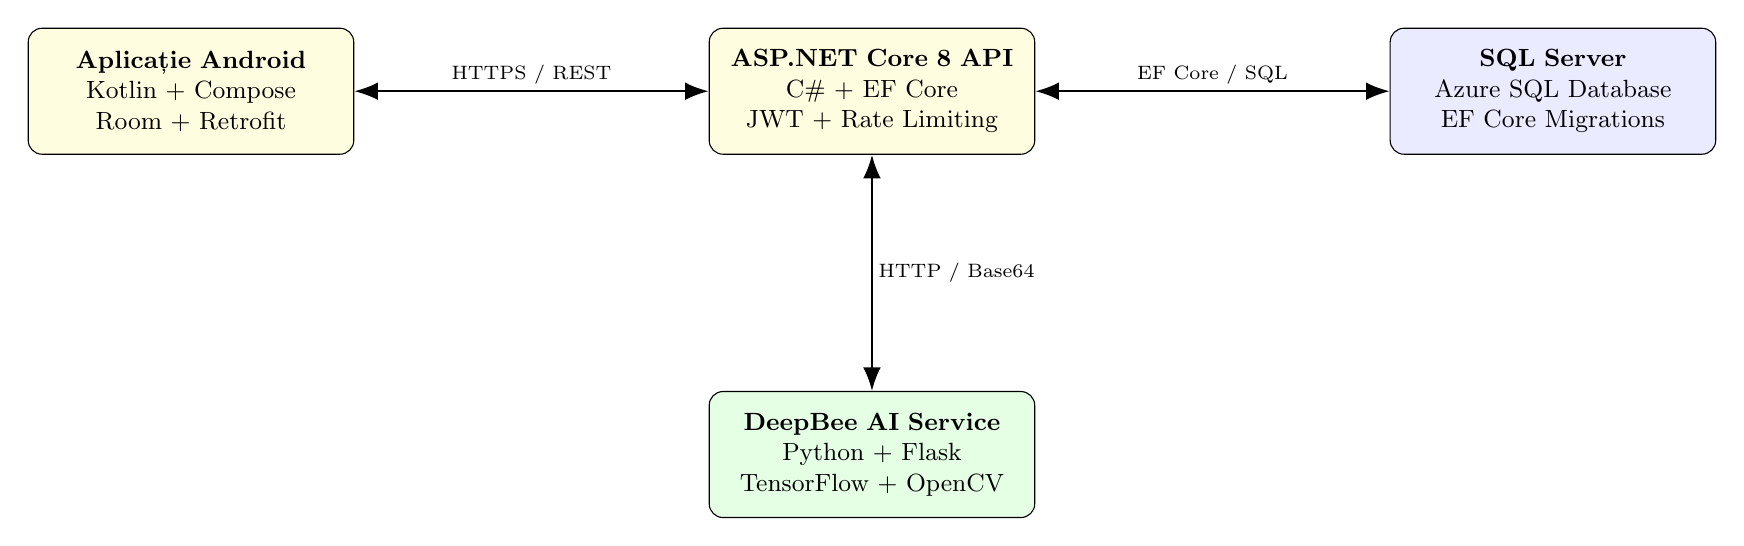
\begin{tikzpicture}[
			cmp/.style={draw, rounded corners=5pt, fill=yellow!12,
				minimum height=1.6cm, text width=3.9cm, align=center, font=\small},
			dbs/.style={draw, rounded corners=5pt, fill=blue!8,
				minimum height=1.6cm, text width=3.9cm, align=center, font=\small},
			ais/.style={draw, rounded corners=5pt, fill=green!10,
				minimum height=1.6cm, text width=3.9cm, align=center, font=\small},
			darr/.style={{Latex[length=3mm]}-{Latex[length=3mm]}, thick},
			lbl/.style={font=\scriptsize, fill=white, inner sep=2pt}
			]
			\node[cmp] (android) {\textbf{Aplicație Android}\\Kotlin + Compose\\Room + Retrofit};
			\node[cmp, right=4.5cm of android] (api) {\textbf{ASP.NET Core 8 API}\\C\# + EF Core\\JWT + Rate Limiting};
			\node[dbs, right=4.5cm of api] (sql) {\textbf{SQL Server}\\Azure SQL Database\\EF Core Migrations};
			\node[ais, below=3cm of api] (ai) {\textbf{DeepBee AI Service}\\Python + Flask\\TensorFlow + OpenCV};
			
			\draw[darr] (android) -- node[lbl, above] {HTTPS / REST} (api);
			\draw[darr] (api)     -- node[lbl, above] {EF Core / SQL} (sql);
			\draw[darr] (api)     -- node[lbl, right] {HTTP / Base64} (ai);
	\end{tikzpicture}}
	\caption{Arhitectura generală a sistemului BeeSmart. Aplicația Android comunică cu backend-ul ASP.NET Core prin HTTPS/REST; backend-ul persistă datele în SQL Server prin Entity Framework Core și apelează serviciul AI pentru analiza fotografiilor de rame. Săgețile duble indică comunicare bidirecțională.}
	\label{fig:arhitectura-generala}
\end{figure}

Separarea responsabilităților reduce dependențele dintre componente. Aplicația Android nu conține modelul AI și nu trebuie să includă biblioteci grele de procesare a imaginilor. Backend-ul rămâne responsabil pentru validarea cererilor, autentificare și persistență, iar serviciul AI poate fi containerizat și actualizat independent de clientul mobil.



\section{Structura proiectului}

Proiectul analizat conține trei zone principale: aplicația Android, backend-ul și documentația. Structura este următoarea:

{\footnotesize
\begin{verbatim}
BeeSmart/
  BeeSmart/                   Aplicația Android
    app/src/main/java/com/example/beesmart/
      data/local/             Room, DAO-uri, entități
      data/repository/        Repository-uri offline-first
      di/                     Module Hilt
      network/                Retrofit, interceptori
      notifications/          Notificări locale
      sync/                   SyncManager/Worker/Scheduler
      ui/                     Compose, Fragmente, ViewModel
      utils/                  Sesiune, fotografii, voce
    gradle/libs.versions.toml Versiuni dependințe

  ApiaryServer/
    ApiaryServer/
      Api/Controllers/        Controllere REST
      Application/            DTO-uri, interfețe, excepții
      Domain/Entities/        Entități de domeniu
      Infrastructure/         DbContext, repository-uri
      AIService/              Serviciu Python (DeepBee)
      docker-compose.yml      SQL Server + API + AI
    ApiaryServer.Tests/       Teste backend
\end{verbatim}
}

\section{Arhitectura aplicației Android}

Aplicația Android urmează un flux de date clar, prezentat în figura~\ref{fig:flux-date-android}.

\begin{figure}[H]
\centering
\resizebox{\textwidth}{!}{%
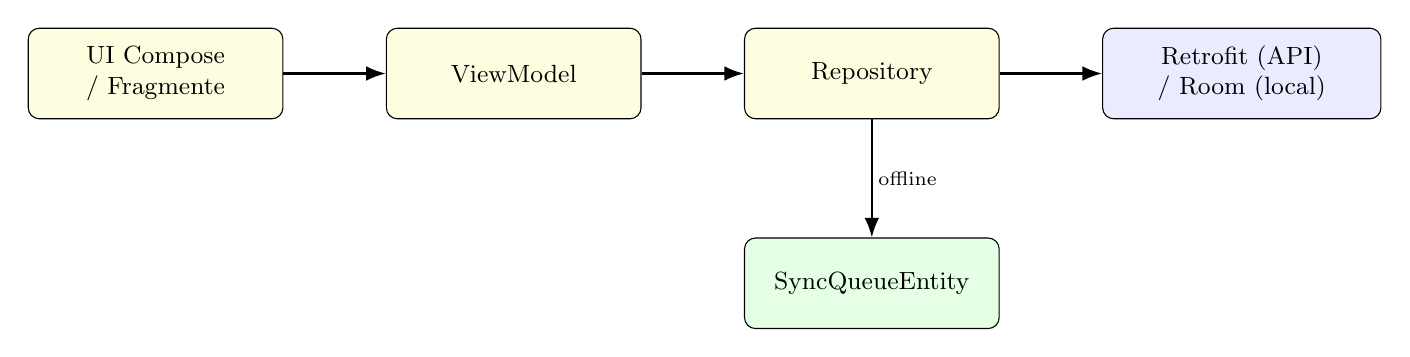
\begin{tikzpicture}[
    box/.style={draw, rounded corners=4pt, fill=yellow!12,
                minimum height=1.15cm, text width=3cm, align=center, font=\small},
    data/.style={draw, rounded corners=4pt, fill=blue!8,
                 minimum height=1.15cm, text width=3.3cm, align=center, font=\small},
    queue/.style={draw, rounded corners=4pt, fill=green!10,
                  minimum height=1.15cm, text width=3cm, align=center, font=\small},
    fl/.style={-{Latex[length=2.5mm]}, thick},
    lbl/.style={font=\scriptsize, fill=white, inner sep=2pt}
]
    \node[box] (ui) {UI Compose / Fragmente};
    \node[box, right=1.3cm of ui] (vm) {ViewModel};
    \node[box, right=1.3cm of vm] (repo) {Repository};
    \node[data, right=1.3cm of repo] (net) {Retrofit (API) / Room (local)};
    \node[queue, below=1.5cm of repo] (queue) {SyncQueueEntity};

    \draw[fl] (ui)   -- (vm);
    \draw[fl] (vm)   -- (repo);
    \draw[fl] (repo) -- (net);
    \draw[fl] (repo) -- node[lbl, right] {offline} (queue);
\end{tikzpicture}}
\caption{Fluxul de date în aplicația Android: acțiunile din interfața Compose sunt transmise prin ViewModel către repository, care alege între accesul online (Retrofit) și cel local (Room); operațiile efectuate offline sunt înregistrate în \texttt{SyncQueueEntity} pentru sincronizare ulterioară.}
\label{fig:flux-date-android}
\end{figure}

Interfața este împărțită pe domenii funcționale: autentificare, acasă, stupine, stupi, inspecții, tratamente, extracții, task-uri, notificări, profil și QR. Fiecare domeniu are propriile ecrane Compose și ViewModel-uri. De exemplu, modulul de inspecții include ecranele \texttt{InspectionListScreen}, \texttt{InspectionFormScreen} și \texttt{InspectionDetailScreen}, împreună cu \texttt{InspectionFormViewModel} și repository-ul \texttt{InspectionRepository}.

\subsubsection*{Pornire, UI și navigare}

La pornire, \texttt{MainActivity} verifică dacă există un deep link activ sau o sesiune autentificată. Dacă utilizatorul nu este autentificat și nu există un deep link de procesat, aplicația afișează mai întâi \texttt{SplashScreen}, un ecran Compose cu animații de prezentare. La finalizarea animației, funcția de continuare declanșează \texttt{runAuthCheck()}, care verifică sesiunea și redirecționează fie spre ecranul principal, fie spre fluxul de autentificare. Această separare a logicii de autentificare în metoda \texttt{runAuthCheck()} permite reutilizarea ei atât din ecranul de pornire, cât și din rutele de deep link, fără duplicare de cod.

Navigarea pornește din \texttt{MainActivity}, care verifică starea autentificării și configurează \texttt{NavController}. \texttt{nav\_graph.xml} definește destinațiile aplicației. Ecranele principale sunt accesibile prin bara de navigație de jos, iar ecranele de creare sau editare sunt ascunse din aceasta pentru a păstra un flux clar.

Aplicația folosește și deep links. În \texttt{AndroidManifest.xml} sunt declarate filtre de intent pentru confirmarea emailului, resetarea parolei și deschiderea fișei unui stup. \texttt{MainActivity} tratează manual parametrii de interogare pentru email și token, deoarece aceste fluxuri trebuie să funcționeze atât prin schema proprie \texttt{beesmart://}, cât și prin adrese HTTPS de forma \texttt{https://app.beesmart.ro/...}.

Sistemul vizual al aplicației este unificat prin componenta \texttt{BeeSmartVisuals}, care definește fundaluri, anteturi de secțiune, panouri de conținut și stări goale reutilizabile în toată interfața. Culorile semantice \texttt{StatusOk}, \texttt{StatusWatch}, \texttt{StatusDanger} și \texttt{StatusInfo} comunică vizual starea unui stup sau a unei operații. Tipografia folosește Plus Jakarta Sans ca font principal și Roboto Mono pentru afișarea valorilor numerice, ambele încărcate prin Google Fonts API.

\subsubsection*{ViewModel-uri și repository-uri}

ViewModel-urile expun stări către UI prin \texttt{StateFlow}. De exemplu, \texttt{HiveDetailViewModel} încarcă detaliile unui stup, ultimele inspecții și analizele AI asociate. \texttt{InspectionFormViewModel} gestionează formularul de inspecție, fotografiile locale, apelul de analiză AI și salvarea rezultatului. Acest model păstrează ecranul Compose concentrat pe afișare și interacțiune, iar logica de date rămâne în ViewModel și repository.

\texttt{UserProfileViewModel} expune două câmpuri care reflectă starea sincronizării: \texttt{pendingSyncCount}, numărul de operații din coada locală care nu au ajuns încă pe server, și \texttt{lastServerSyncMillis}, momentul ultimei sincronizări reale confirmate cu serverul. Aceste valori sunt afișate în \texttt{UserProfileScreen}, astfel încât utilizatorul să poată verifica dacă datele introduse în teren sunt sincronizate. \texttt{SessionManager} primește apeluri \texttt{markServerSyncNow()} din \texttt{SyncManager} și din \texttt{UserProfileRepository} ori de câte ori o sincronizare cu serverul se finalizează cu succes.

Repository-urile constituie punctul de decizie al stratului de date Android. Ele stabilesc dacă o operație se execută online, prin Retrofit, sau offline, prin Room. \texttt{ApiaryRepository}, de exemplu, verifică \texttt{ConnectivityObserver} și \texttt{BackendReachability}. Dacă backend-ul nu este disponibil, creează o entitate locală cu \texttt{PENDING\_CREATE} și introduce un rând în \texttt{SyncQueueEntity}. Dacă backend-ul este disponibil, trimite cererea la server și salvează răspunsul în Room.

Aceeași strategie este folosită pentru stupi, task-uri, tratamente, extracții, inspecții și fotografii. În cazul analizei AI, repository-ul impune conexiune la backend, deoarece modelul rulează în serviciul AI.

\section{Arhitectura backend}

Backend-ul este organizat în patru straturi:

\begin{verbatim}
Api -> Application -> Domain -> Infrastructure
\end{verbatim}

Stratul \texttt{Api} conține controllerele HTTP. Stratul \texttt{Application} definește DTO-uri, interfețe, excepții și clase de opțiuni. Stratul \texttt{Domain} conține entitățile de business. Stratul \texttt{Infrastructure} include \texttt{AppDbContext}, repository-urile, serviciile, logica de email, JWT și integrarea cu serviciul AI.

Controllerele sunt declarate în \texttt{Api/Controllers}. \texttt{AuthController} gestionează înregistrarea, autentificarea, reîmprospătarea token-ului, confirmarea emailului, resetarea parolei și profilul. \texttt{ApiaryController}, \texttt{HiveController}, \texttt{InspectionController}, \texttt{TaskController}, \texttt{HiveTreatmentController} și \texttt{HiveExtractionController} expun operațiile CRUD pentru entitățile apicole.

Rutele protejate folosesc atributul \texttt{[Authorize]}. Identitatea utilizatorului este extrasă din \texttt{ClaimTypes.NameIdentifier}. Serviciile verifică apoi dacă resursa aparține utilizatorului curent. Această verificare este necesară deoarece un token valid nu trebuie să permită accesul la stupinele altui utilizator.

Backend-ul aplică o limitare a numărului de cereri, configurată în \texttt{Program.cs} prin \texttt{AddRateLimiter}. Există trei politici distincte. Prima este un limitator global, care restricționează fiecare adresă IP la 120 de cereri pe minut, cu o coadă de așteptare de cel mult 20 de cereri suplimentare. A doua politică, numită \texttt{fixed}, limitează rutele generice la 5 cereri pe minut. A treia, numită \texttt{login}, restricționează ruta de autentificare la 5 încercări pe minut fără coadă de așteptare, pentru a preveni atacurile prin forță brută.

Adresele IP sunt extrase corect și atunci când aplicația rulează în spatele unui proxy sau al Azure Container Apps, deoarece \texttt{UseForwardedHeaders} este configurat cu \texttt{XForwardedFor} și \texttt{XForwardedProto}, cu rețelele cunoscute golite pentru a accepta orice proxy de încredere. Cererile respinse primesc codul HTTP 429.

Serviciile din \texttt{Infrastructure/Services} conțin logica de business. De exemplu, \texttt{InspectionService} verifică dacă stupul există și aparține utilizatorului înainte de a crea o inspecție. La salvarea unei analize AI, același serviciu normalizează clasele întoarse de AI, calculează indicatorii derivați și persistă rezultatul în tabela \texttt{InspectionAiAnalyses}.

Repository-urile din \texttt{Infrastructure/Repositories} izolează accesul la baza de date. Ele folosesc \texttt{AppDbContext} și includ metode pentru interogări pe utilizator, căutări după id, adăugare, actualizare, ștergere și verificări de apartenență. Această separare face ca serviciile să nu depindă direct de detalii EF Core în fiecare metodă.

\section{Modelul bazei de date}

Pe server, baza de date este definită prin \texttt{AppDbContext}. Entitățile principale sunt:
\begin{itemize}
	\item \texttt{User}: contul utilizatorului, email, parolă hash-uită, profil, confirmare email;
	\item \texttt{RefreshToken}, \texttt{EmailConfirmationToken}, \texttt{PasswordResetToken}: token-uri pentru securitate și fluxuri de cont;
	\item \texttt{Apiary}: stupină asociată unui utilizator, cu nume, descriere și locație;
	\item \texttt{Hive}: stup asociat unei stupine, cu tip, status, note, date despre matcă și rame;
	\item \texttt{Inspection}: inspecție asociată unui stup și unei stupine;
	\item \texttt{InspectionPhoto}: fotografie atașată unei inspecții;
	\item \texttt{InspectionAiAnalysis}: rezultatul salvat al unei analize DeepBee;
	\item \texttt{HiveTreatment}: tratament aplicat unui stup;
	\item \texttt{HiveExtraction}: extracție de miere, polen, propolis, ceară sau alt produs;
	\item \texttt{HiveTask}: sarcină asociată unui utilizator, opțional unei stupine sau unui stup.
\end{itemize}

Relațiile sunt configurate explicit. Un utilizator deține stupine, o stupină conține stupi, un stup conține inspecții, tratamente și extracții. O inspecție poate avea fotografii și analize AI. Pentru task-uri, relațiile cu stupina și stupul folosesc \texttt{DeleteBehavior.NoAction}, pentru a evita conflictele de cascade în SQL Server. Modelul entităților principale și relațiile dintre ele sunt prezentate în figura~\ref{fig:er-diagram}.

Local, Room are un model asemănător, dar adaptat sincronizării. Entitățile locale includ câmpuri precum \texttt{localId}, \texttt{serverId}, \texttt{syncStatus} și \texttt{updatedAt}. În plus, există \texttt{SyncQueueEntity}, care nu există pe server, deoarece reprezintă mecanismul clientului pentru memorarea operațiilor offline.

\begin{figure}[H]
\centering
\resizebox{\textwidth}{!}{%
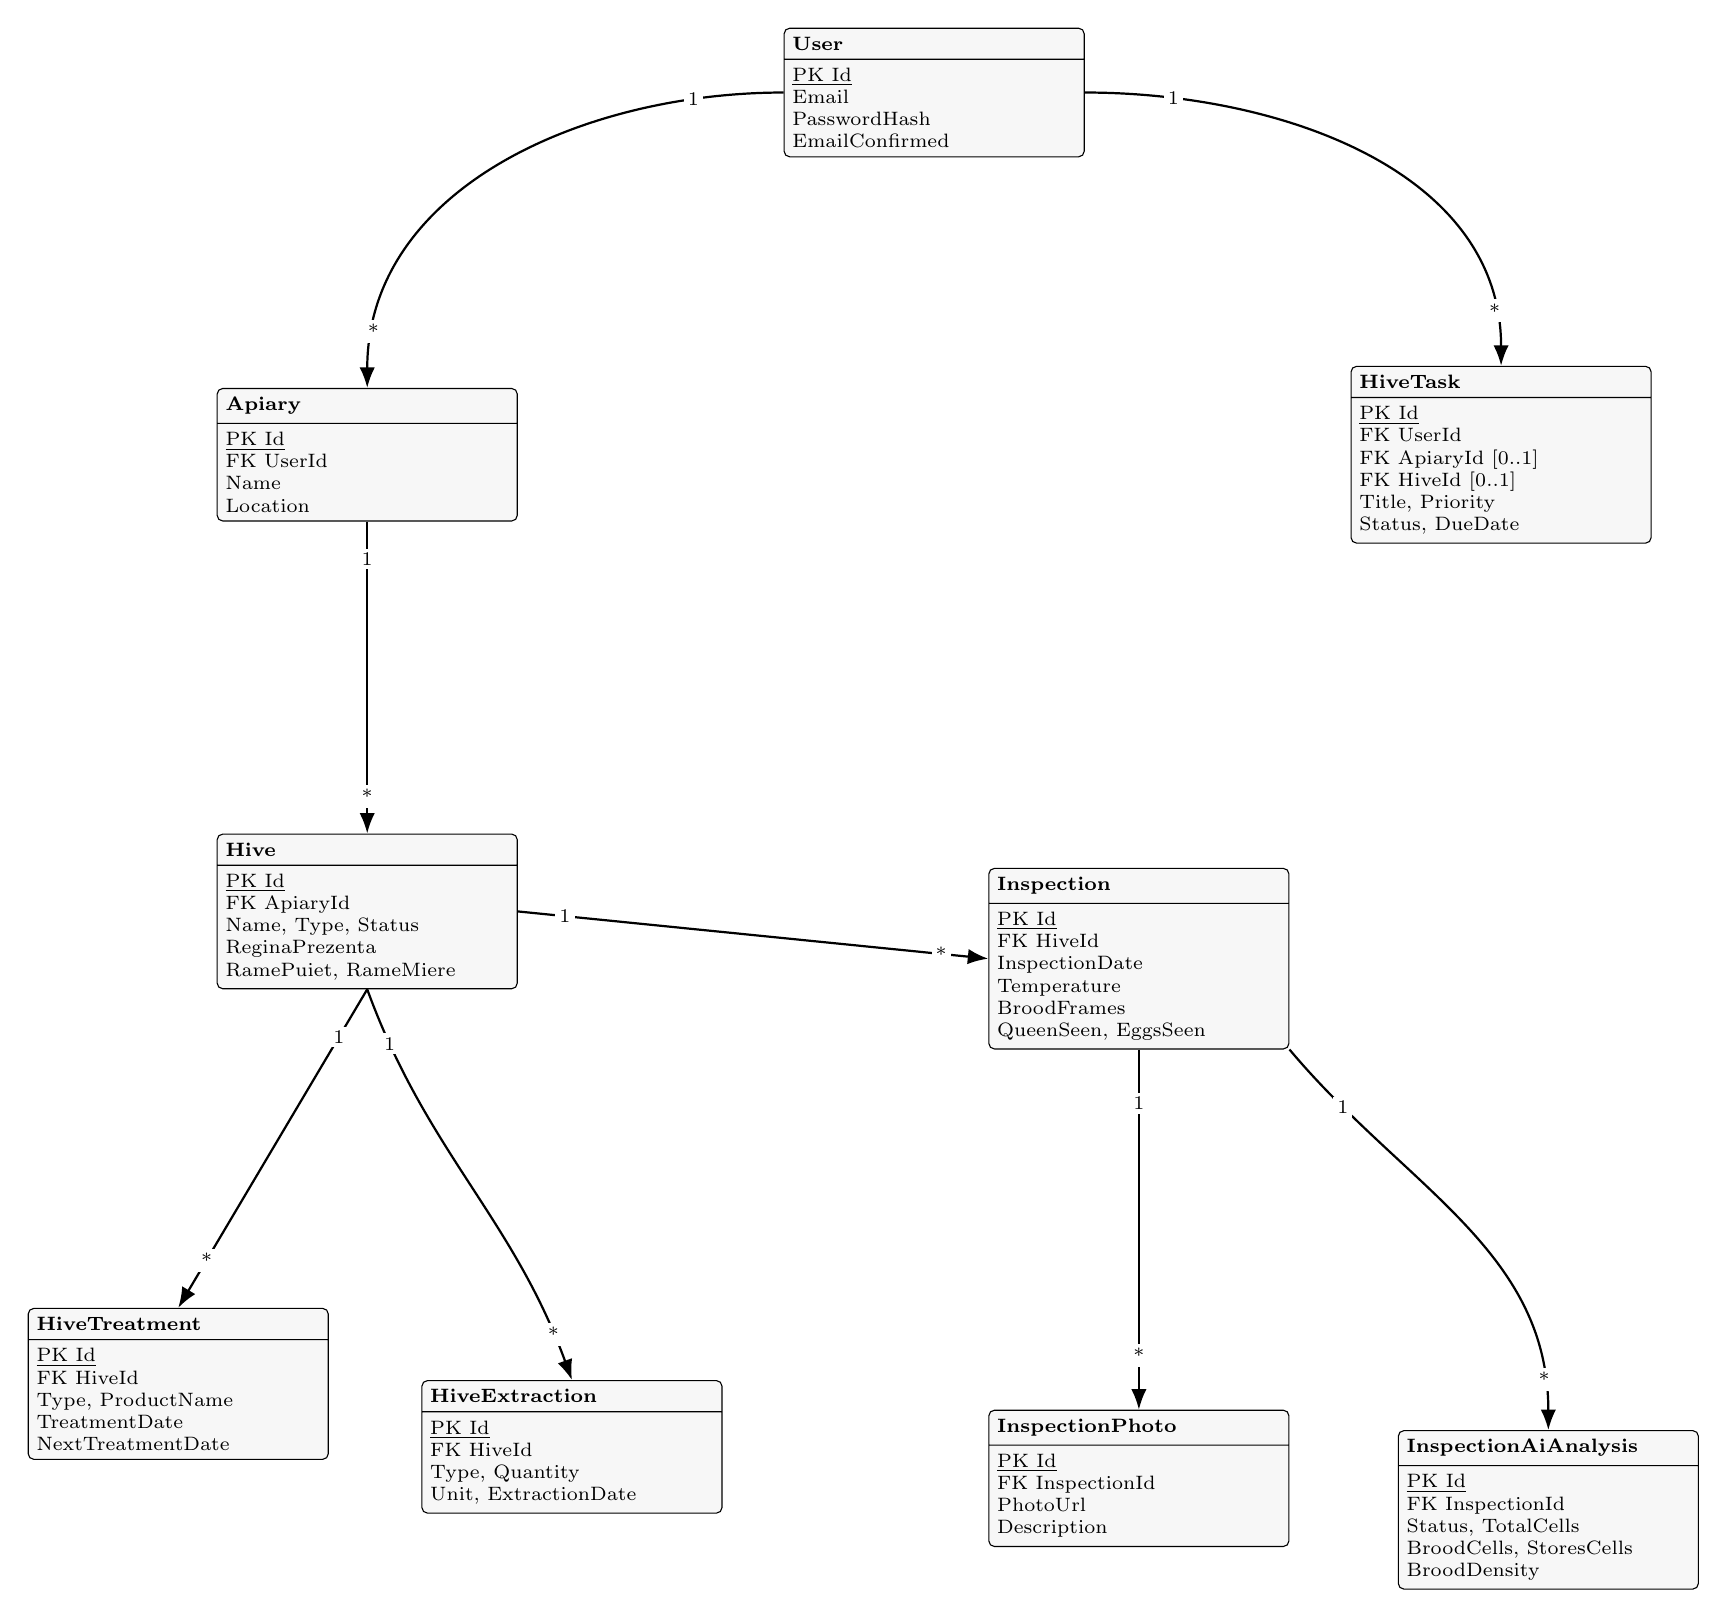
\begin{tikzpicture}[
    entity/.style={draw, rounded corners=2pt, fill=gray!6,
                rectangle split, rectangle split parts=2,
                rectangle split draw splits=true,
                text width=3.6cm, align=left, font=\scriptsize,
                inner sep=3pt},
    title/.style={font=\scriptsize\bfseries},
    arr/.style={-{Latex[length=2.6mm]}, thick},
    one/.style={font=\scriptsize, fill=white, inner sep=1.5pt},
    many/.style={font=\scriptsize, fill=white, inner sep=1.5pt}
]
    \node[entity] (user) at (0,0)
        {\nodepart[title]{one}User
         \nodepart{two}\underline{PK Id}\\ Email\\ PasswordHash\\ EmailConfirmed};

    \node[entity] (apiary) at (-7.2,-4.6)
        {\nodepart[title]{one}Apiary
         \nodepart{two}\underline{PK Id}\\ FK UserId\\ Name\\ Location};

    \node[entity] (task) at (7.2,-4.6)
        {\nodepart[title]{one}HiveTask
         \nodepart{two}\underline{PK Id}\\ FK UserId\\ FK ApiaryId [0..1]\\ FK HiveId [0..1]\\ Title, Priority\\ Status, DueDate};

    \node[entity] (hive) at (-7.2,-10.4)
        {\nodepart[title]{one}Hive
         \nodepart{two}\underline{PK Id}\\ FK ApiaryId\\ Name, Type, Status\\ ReginaPrezenta\\ RamePuiet, RameMiere};

    \node[entity] (inspection) at (2.6,-11.0)
        {\nodepart[title]{one}Inspection
         \nodepart{two}\underline{PK Id}\\ FK HiveId\\ InspectionDate\\ Temperature\\ BroodFrames\\ QueenSeen, EggsSeen};

    \node[entity] (treatment) at (-9.6,-16.4)
        {\nodepart[title]{one}HiveTreatment
         \nodepart{two}\underline{PK Id}\\ FK HiveId\\ Type, ProductName\\ TreatmentDate\\ NextTreatmentDate};

    \node[entity] (extraction) at (-4.6,-17.2)
        {\nodepart[title]{one}HiveExtraction
         \nodepart{two}\underline{PK Id}\\ FK HiveId\\ Type, Quantity\\ Unit, ExtractionDate};

    \node[entity] (photo) at (2.6,-17.6)
        {\nodepart[title]{one}InspectionPhoto
         \nodepart{two}\underline{PK Id}\\ FK InspectionId\\ PhotoUrl\\ Description};

    \node[entity] (aianalysis) at (7.8,-18.0)
        {\nodepart[title]{one}InspectionAiAnalysis
         \nodepart{two}\underline{PK Id}\\ FK InspectionId\\ Status, TotalCells\\ BroodCells, StoresCells\\ BroodDensity};

    \draw[arr] (user.west)    to[out=180,in=90]  node[one,pos=0.15]{1} node[many,pos=0.9]{*} (apiary.north);
    \draw[arr] (user.east)    to[out=0,in=90]    node[one,pos=0.15]{1} node[many,pos=0.9]{*} (task.north);
    \draw[arr] (apiary.south) -- node[one,pos=0.12]{1} node[many,pos=0.88]{*} (hive.north);
    \draw[arr] (hive.east)    -- node[one,pos=0.1]{1} node[many,pos=0.9]{*} (inspection.west);
    \draw[arr] (hive.south)   -- node[one,pos=0.15]{1} node[many,pos=0.85]{*} (treatment.north);
    \draw[arr] (hive.south)   to[out=-70,in=110] node[one,pos=0.12]{1} node[many,pos=0.9]{*} (extraction.north);
    \draw[arr] (inspection.south) -- node[one,pos=0.15]{1} node[many,pos=0.85]{*} (photo.north);
    \draw[arr] (inspection.south east) to[out=-50,in=90] node[one,pos=0.15]{1} node[many,pos=0.9]{*} (aianalysis.north);
\end{tikzpicture}}
\caption{Diagrama entităților principale ale bazei de date BeeSmart, cu atributele-cheie și marcajele de cheie primară (\underline{PK}) și cheie externă (FK). Relațiile sunt de tip unu-la-mulți (\enquote{1} la părinte, \enquote{*} la copil). Entitatea \texttt{HiveTask} poate referenția opțional o stupină sau un stup, marcaj redat prin \texttt{[0..1]} pe câmpurile \texttt{ApiaryId} și \texttt{HiveId}.}
\label{fig:er-diagram}
\end{figure}

\section{Mecanismul offline-first}

În BeeSmart, strategia offline-first reprezintă mecanismul prin care aplicația rămâne utilizabilă în stupină, chiar și atunci când conexiunea la internet lipsește sau este instabilă. Spre deosebire de un flux exclusiv online, în care o cerere de creare depinde imediat de răspunsul serverului, repository-ul verifică mai întâi accesibilitatea backend-ului. Dacă acesta nu poate fi contactat, datele sunt persistate în Room, iar operația este înregistrată în coada de sincronizare pentru transmiterea ulterioară.

\subsubsection*{Creare, actualizare și ștergere offline}

La crearea offline a unei stupine, \texttt{ApiaryRepository} generează un UUID local, creează un \texttt{ApiaryEntity} cu \texttt{serverId = null} și \texttt{syncStatus = PENDING\_CREATE}, apoi adaugă în \texttt{sync\_queue} o operație de tip \texttt{CREATE}. UI-ul primește imediat un răspuns de succes, deoarece operația a fost salvată local. Utilizatorul poate continua munca fără să aștepte serverul.

Pentru entitățile copil, cum ar fi stupii sau inspecțiile, localId-ul părintelui este păstrat până când serverul returnează un id real. \texttt{SyncManager} rezolvă ulterior acest id. Dacă stupul depinde de o stupină care încă nu s-a sincronizat, operația este amânată, nu eșuată.

Actualizările offline sunt salvate local cu \texttt{PENDING\_UPDATE}, iar conținutul cererii este păstrat în coadă. Ștergerile offline sunt tratate diferit în funcție de existența unui \texttt{serverId}. Dacă entitatea nu a fost sincronizată niciodată, ea poate fi ștearsă local și operația de creare din coadă este eliminată. Dacă entitatea există deja pe server, este marcată \texttt{PENDING\_DELETE}, iar coada va trimite o cerere DELETE când conexiunea revine.

\subsubsection*{Procesarea cozii}

\texttt{SyncManager.processQueue()} citește toate operațiile și le grupează după tip. Creările sunt procesate în ordine de dependență: mai întâi stupinele, apoi stupii, apoi task-urile, tratamentele, extracțiile, inspecțiile și fotografiile. Actualizările, ștergerile și acțiunile de completare/decompletare a task-urilor sunt procesate ulterior. Această ordine este verificată de testele de integrare.

La sincronizarea actualizărilor și ștergerilor de fotografii, \texttt{SyncManager} rezolvă mai întâi id-ul de server al fotografiei folosind o nouă interogare DAO \texttt{getLatestQueuedOperationForEntity()}, care returnează ultima operație înregistrată în coadă pentru o entitate dată. Acest mecanism previne situațiile în care o actualizare de fotografie este trimisă cu un id local, invalid din perspectiva serverului.

Erorile sunt tratate diferit. Dacă apare o eroare de rețea de tip \texttt{IOException}, operația rămâne în coadă fără creșterea numărului de reîncercări. Dacă serverul răspunde cu o eroare HTTP, numărul de reîncercări crește. La 3 încercări, entitatea este marcată \texttt{SYNC\_FAILED}. Această politică evită consumarea reîncercărilor pentru probleme temporare de conectivitate.

\section{Fluxul AI}

Fluxul AI pornește în ecranul de inspecție. Utilizatorul adaugă o fotografie, iar \texttt{InspectionFormViewModel} o transformă în Base64 prin \texttt{PhotoManager}. Cererea este trimisă la ruta Android Retrofit \texttt{POST inspections/analyze-cells}. Backend-ul primește \texttt{AnalyzeCellsRequest}, validează faptul că imaginea este Base64 valid și apelează \texttt{AiAnalysisService}.

\texttt{AiAnalysisService} trimite conținutul cererii către serviciul Python, la ruta configurată \texttt{/analyze}. Serviciul AI decodează imaginea, verifică parametrii de calitate, detectează celulele și clasifică regiunile. Răspunsul se întoarce la backend și apoi la aplicația Android.

\begin{figure}[H]
	\centering
	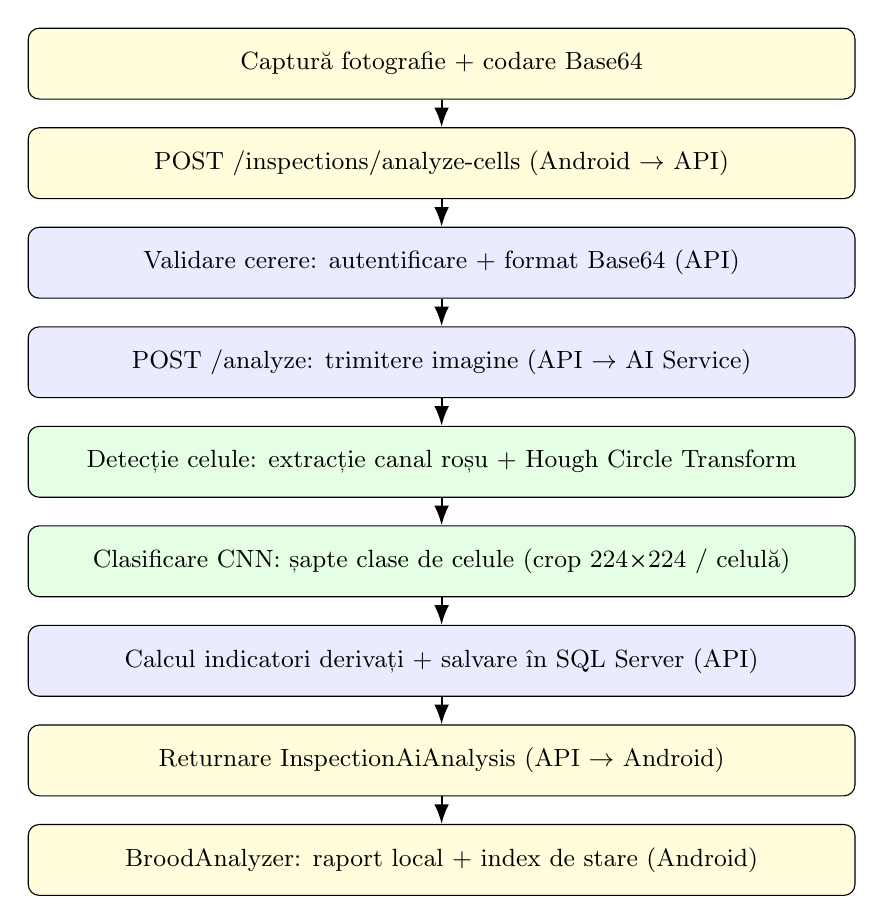
\begin{tikzpicture}[
		anode/.style={draw, rounded corners=4pt, fill=yellow!14,
			minimum width=10.5cm, minimum height=0.9cm, align=center, font=\small},
		bnode/.style={draw, rounded corners=4pt, fill=blue!8,
			minimum width=10.5cm, minimum height=0.9cm, align=center, font=\small},
		cnode/.style={draw, rounded corners=4pt, fill=green!10,
			minimum width=10.5cm, minimum height=0.9cm, align=center, font=\small},
		arr/.style={-{Latex[length=2.5mm]}, thick}
		]
		\node[anode] (s1) {Captură fotografie + codare Base64};
		\node[anode, below=0.35cm of s1] (s2) {POST /inspections/analyze-cells (Android $\rightarrow$ API)};
		\node[bnode, below=0.35cm of s2] (s3) {Validare cerere: autentificare + format Base64 (API)};
		\node[bnode, below=0.35cm of s3] (s4) {POST /analyze: trimitere imagine (API $\rightarrow$ AI Service)};
		\node[cnode, below=0.35cm of s4] (s5) {Detecție celule: extracție canal roșu + Hough Circle Transform};
		\node[cnode, below=0.35cm of s5] (s6) {Clasificare CNN: șapte clase de celule (crop 224×224 / celulă)};
		\node[bnode, below=0.35cm of s6] (s7) {Calcul indicatori derivați + salvare în SQL Server (API)};
		\node[anode, below=0.35cm of s7] (s8) {Returnare InspectionAiAnalysis (API $\rightarrow$ Android)};
		\node[anode, below=0.35cm of s8] (s9) {BroodAnalyzer: raport local + index de stare (Android)};
		
		\foreach \s/\t in {s1/s2, s2/s3, s3/s4, s4/s5, s5/s6, s6/s7, s7/s8, s8/s9}
		\draw[arr] (\s) -- (\t);
	\end{tikzpicture}
	\caption{Fluxul complet al analizei AI în BeeSmart. Pașii \textit{galben} rulează pe Android, pașii \textit{albastru} pe backend-ul ASP.NET Core, iar pașii \textit{verde} pe serviciul Python DeepBee.}
	\label{fig:flux-ai}
\end{figure}

După ce analiza este primită, \texttt{InspectionFormViewModel} folosește \texttt{BroodAnalyzer} pentru a construi un raport local: total celule, categorii, evidențieri, probleme posibile și recomandări. Dacă inspecția este deja salvată, analiza este persistată imediat local și se încearcă salvarea pe server. Dacă inspecția este nouă, analiza este păstrată temporar și se salvează după ce inspecția primește id-ul corespunzător. Traseul complet, de la captarea fotografiei până la salvarea rezultatului, este prezentat în figura~\ref{fig:flux-ai}.



\section{Statistici și index de stare pe stup}

Rezultatele AI nu sunt afișate doar ca un dicționar brut. Backend-ul salvează indicatori precum \texttt{TotalCells}, \texttt{BroodCells}, \texttt{StoresCells}, \texttt{BroodDensity}, \texttt{LarvaeToCappedRatio} și \texttt{StoresRatio}. Pe Android, \texttt{HiveStatsScreen} folosește aceste valori pentru a afișa:
\begin{itemize}
	\item numărul de celule analizate;
	\item indexul curent;
	\item numărul de celule de puiet și rezerve;
	\item tendința față de analiza anterioară;
	\item evoluția lunară pe anul curent;
	\item comparația inter-anuală pentru aceeași lună;
	\item distribuția celulelor și interpretări apicole.
\end{itemize}

Indexul compozit folosit în UI este calculat din densitatea puietului și rezerve, cu penalizare când raportul larve/puiet căpăcit este foarte scăzut. Textul din interfață precizează că valorile sunt suport decizional, nu diagnostic veterinar. Această formulare este importantă pentru responsabilitatea aplicației.

\section{Indicatori de stupină și consilier contextual}

Pe lângă statisticile individuale ale stupilor, aplicația calculează un set de indicatori agregați la nivelul întregii stupine, afișați pe ecranul principal (\texttt{HomeScreen}). Aceste calcule sunt realizate de trei clase distincte din pachetul \texttt{data/repository}: \texttt{ApiaryIntelligenceCalculator}, \texttt{DashboardAnalyticsCalculator} și \texttt{DeepBeeContextAdvisor}. Calculele sunt efectuate local, pe baza datelor deja disponibile în Room, fără a necesita apeluri suplimentare la server. \texttt{HomeRepository} prelucrează instantaneele de analiză AI stocate prin Moshi și le pune la dispoziția calculatoarelor ca obiecte \texttt{AiHiveSnapshot}.

\subsubsection*{Indexul de risc per stup}

\texttt{ApiaryIntelligenceCalculator} produce un obiect \texttt{ApiaryRadar} care conține scorul mediu de sănătate al stupinei, numărul de stupi monitorizați, distribuția acestora în categoriile \texttt{STABLE}, \texttt{WATCH} și \texttt{CRITICAL}, procentul de acoperire cu inspecții și numărul de stupi cu cel puțin o analiză DeepBee salvată.

Evaluarea fiecărui stup se bazează pe un sistem de penalizări cu puncte. Statusul stupului (bolnav, orfan, slab) adaugă cel mai mare număr de puncte de risc. Absența confirmării reginei, lipsa puietului raportat, vechimea mătcii peste doi ani, inspecțiile întârziate, task-urile critice deschise și semnalele AI de avertizare adaugă penalizări suplimentare. Dacă notăm cu $p_i$ penalizarea asociată fiecărui factor de risc $i$ dintr-o mulțime $F$, scorul de sănătate al stupului este definit ca
\begin{equation}
	H = \operatorname{clamp}_{[0,100]}\!\left(100 - \sum_{i \in F} p_i\right),
	\qquad
	\operatorname{clamp}_{[0,100]}(x) = \min\bigl(100, \max(0, x)\bigr).
	\label{eq:scor-sanatate}
\end{equation}
Clasificarea stupului este apoi
\begin{equation}
	\text{categorie}(H) =
	\begin{cases}
		\texttt{CRITICAL}, & H < 50,\\
		\texttt{WATCH},    & 50 \le H \le 80,\\
		\texttt{STABLE},   & H > 80.
	\end{cases}
	\label{eq:categorie-stup}
\end{equation}
Operatorul de saturare din relația \eqref{eq:scor-sanatate} garantează că scorul rămâne în intervalul $[0, 100]$ chiar și atunci când suma penalizărilor depășește 100. Fiecare penalizare $p_i$ generează un mesaj de motiv și o acțiune recomandată, afișate în ordinea priorităților.

\subsubsection*{Producție, prognoză și consilier contextual}

\texttt{DashboardAnalyticsCalculator} este punctul de intrare care orchestrează celelalte două calculatoare și returnează un obiect \texttt{DashboardStats} complet. Pe lângă apelarea \texttt{ApiaryIntelligenceCalculator} și \texttt{DeepBeeContextAdvisor}, calculează analiza de producție (\texttt{HoneyAnalytics}).

Producția de miere extrasă este agregată din înregistrările de extracții de tip \texttt{Honey}. Aplicația normalizează unitățile (kg și g), ignoră intrările cu cantitate negativă sau nenumerică și calculează producția lunară din ultimele șase luni. Prognoza pentru recolta următoare este estimată din capacitatea teoretică a ramelor cu miere ale stupilor activi, ținând cont de tipul stupului: pentru stupii Dadant se folosește o capacitate de 3,6 kg per ramă pe deplin căpăcită, iar pentru celelalte tipuri 2,3 kg. Prognoza este exprimată ca interval minim--mediu--maxim, iar nivelul de încredere al estimării depinde de numărul de înregistrări istorice și de stupii cu rame cu miere declarate.

\texttt{DeepBeeContextAdvisor} produce un \texttt{ApiaryAdviceDigest} care conține sfaturi prioritizate pe patru niveluri: \texttt{URGENT}, \texttt{IMPORTANT}, \texttt{WATCH} și \texttt{OPPORTUNITY}. Fiecare sfat (\texttt{BeekeeperAdvice}) include un titlu, o explicație, o acțiune propusă, o listă de dovezi extrase din date și un indicator opțional de recomandare pentru evaluare de specialitate. Sfaturile sunt generate per stup și sortate global după prioritate.

Logica consilierului combină mai multe surse de date: starea mătcii (din câmpurile stupului, din inspecție și din analiza AI), semnalele de roire (botci cu ouă, barbă la urdiniș, presiunea de spațiu calculată atât din numărul de rame, cât și din raportul AI al celulelor goale), tendința puietului, rezervele de hrană, tratamentele Varroa înregistrate, termenele expirate de tratament, task-urile critice sau întârziate și calendarul sezonier. Sfaturile sezoniere (primăvară, vară, toamnă, iarnă) sunt omise dacă există deja un task cu titlu corespunzător, pentru a evita duplicarea.

Un aspect esențial al proiectării este că consilierul nu emite diagnostice veterinare și nu prescrie tratamente. Fiecare sfat conține explicit dovezile pe care se bazează, astfel încât utilizatorul să poată valida concluzia din teren înainte de a acționa. Această delimitare este menținută atât în cod, cât și în textele afișate în interfață.

\section{Autentificare, email și deep links}

Fluxul de autentificare este realizat prin \texttt{ComposeAuthActivity} și ecranele de autentificare, înregistrare, recuperare a parolei și resetare a parolei. Backend-ul oferă rute pentru înregistrare, autentificare, reîmprospătarea token-ului, confirmarea emailului și resetarea parolei. Email-urile folosesc configurarea SMTP din \texttt{appsettings.json}, iar adresele pot folosi schema proprie \texttt{beesmart://} sau domeniul web \texttt{https://app.beesmart.ro}.

Deep link-urile sunt folosite și pentru QR. \texttt{QrCodeUtils} generează un cod QR cu adresa către stup, iar \texttt{QrScannerScreen} scanează codul cu CameraX și ML Kit. Dacă adresa este validă, aplicația extrage id-ul stupului și navighează către ecranul de editare. Acest mecanism este util în stupină: fiecare stup poate avea o etichetă fizică, iar apicultorul poate deschide direct datele lui.

\section{Notificări locale}

\subsubsection*{Notificări pentru task-uri și tratamente}

Task-urile permit planificarea activităților legate de o stupină sau de un stup. Ele au titlu, descriere, prioritate, status, termen limită și, opțional, moment de finalizare. Pe Android, notificările locale pentru task-uri sunt gestionate prin \texttt{TaskNotificationScheduler}, care folosește \texttt{AlarmManager}. Pentru fiecare task cu termen limită se pot programa notificări în ziua precedentă și în ziua termenului.

Tratamentele cu termen de reaplicare pot declanșa notificări locale independente. \texttt{Treatment\-Notification\-Scheduler} primește id-ul tratamentului, numele produsului și data de reaplicare, calculează marcajul temporal corespunzător orei 08:00 a zilei respective și programează o alarmă prin \texttt{Alarm\-Manager.\-setExact\-And\-Allow\-While\-Idle()}, care funcționează chiar și atunci când dispozitivul se află în modul de economisire a energiei. Pe Android 12 și versiunile superioare este verificat mai întâi dacă aplicația are permisiunea de a programa alarme exacte; în absența acesteia, se folosește \texttt{set()}, care nu garantează precizia la minut, dar livrează totuși notificarea.

Notificarea este livrată de \texttt{TreatmentNotificationReceiver}, un \texttt{BroadcastReceiver} care primește datele din Intent și afișează notificarea prin canalul de notificări al aplicației. \texttt{BootCompleteReceiver} reprogramează toate alarmele de tratament după repornirea dispozitivului, deoarece Android șterge alarmele la repornire. Această arhitectură garantează că utilizatorul primește reamintirile chiar dacă dispozitivul a fost oprit și repornit între momentul programării și momentul declanșării notificării.

Istoricul notificărilor este păstrat local în \texttt{NotificationHistoryEntity}, cu titlu, mesaj, tip, entitate asociată, data creării și starea citit/necitit. Această funcție nu este echivalentă cu un sistem de notificări push de la server, ci reprezintă notificări locale pentru organizarea activității utilizatorului.
\chapter{Descriere funcțională și validare}
\label{chap:functionalitati}

\section{Prezentarea interfeței grafice}

Interfața BeeSmart este construită pentru un utilizator care lucrează în teren și are nevoie de acces rapid la informații. La prima pornire fără sesiune activă, aplicația afișează un ecran de splash cu animații de prezentare, după care trece automat la fluxul de autentificare. Odată autentificat, utilizatorul ajunge pe ecranul principal, de unde poate naviga către stupine, inspecții, task-uri, profil și alte funcționalități. Navigarea principală este realizată prin bara de navigație de jos, iar ecranele de creare sau editare se deschid ca fluxuri dedicate.

Designul folosește ecrane Compose structurate pe carduri, liste și formulare. Componentele reutilizabile \texttt{BeeSmartPanel} și \texttt{BeeSmartEmptyState} unifică aspectul tuturor ecranelor. Culorile semantice \texttt{StatusOk}, \texttt{StatusWatch} și \texttt{StatusDanger} comunică vizual nivelul de atenție necesar pentru un stup sau o operație. Fiecare zonă funcțională are stări clare: încărcare, succes, eroare sau stare goală. De exemplu, ecranul de statistici DeepBee afișează un mesaj dacă nu există încă analize AI pentru stupul curent, iar ecranul meteo afișează o stare indisponibilă dacă cheia OpenWeatherMap nu este configurată. Ecranul principal al aplicației este prezentat în figura~\ref{fig:home}.

\begin{figure}[H]
	\centering
	\subfigure[Salut și sumarul stupinei]{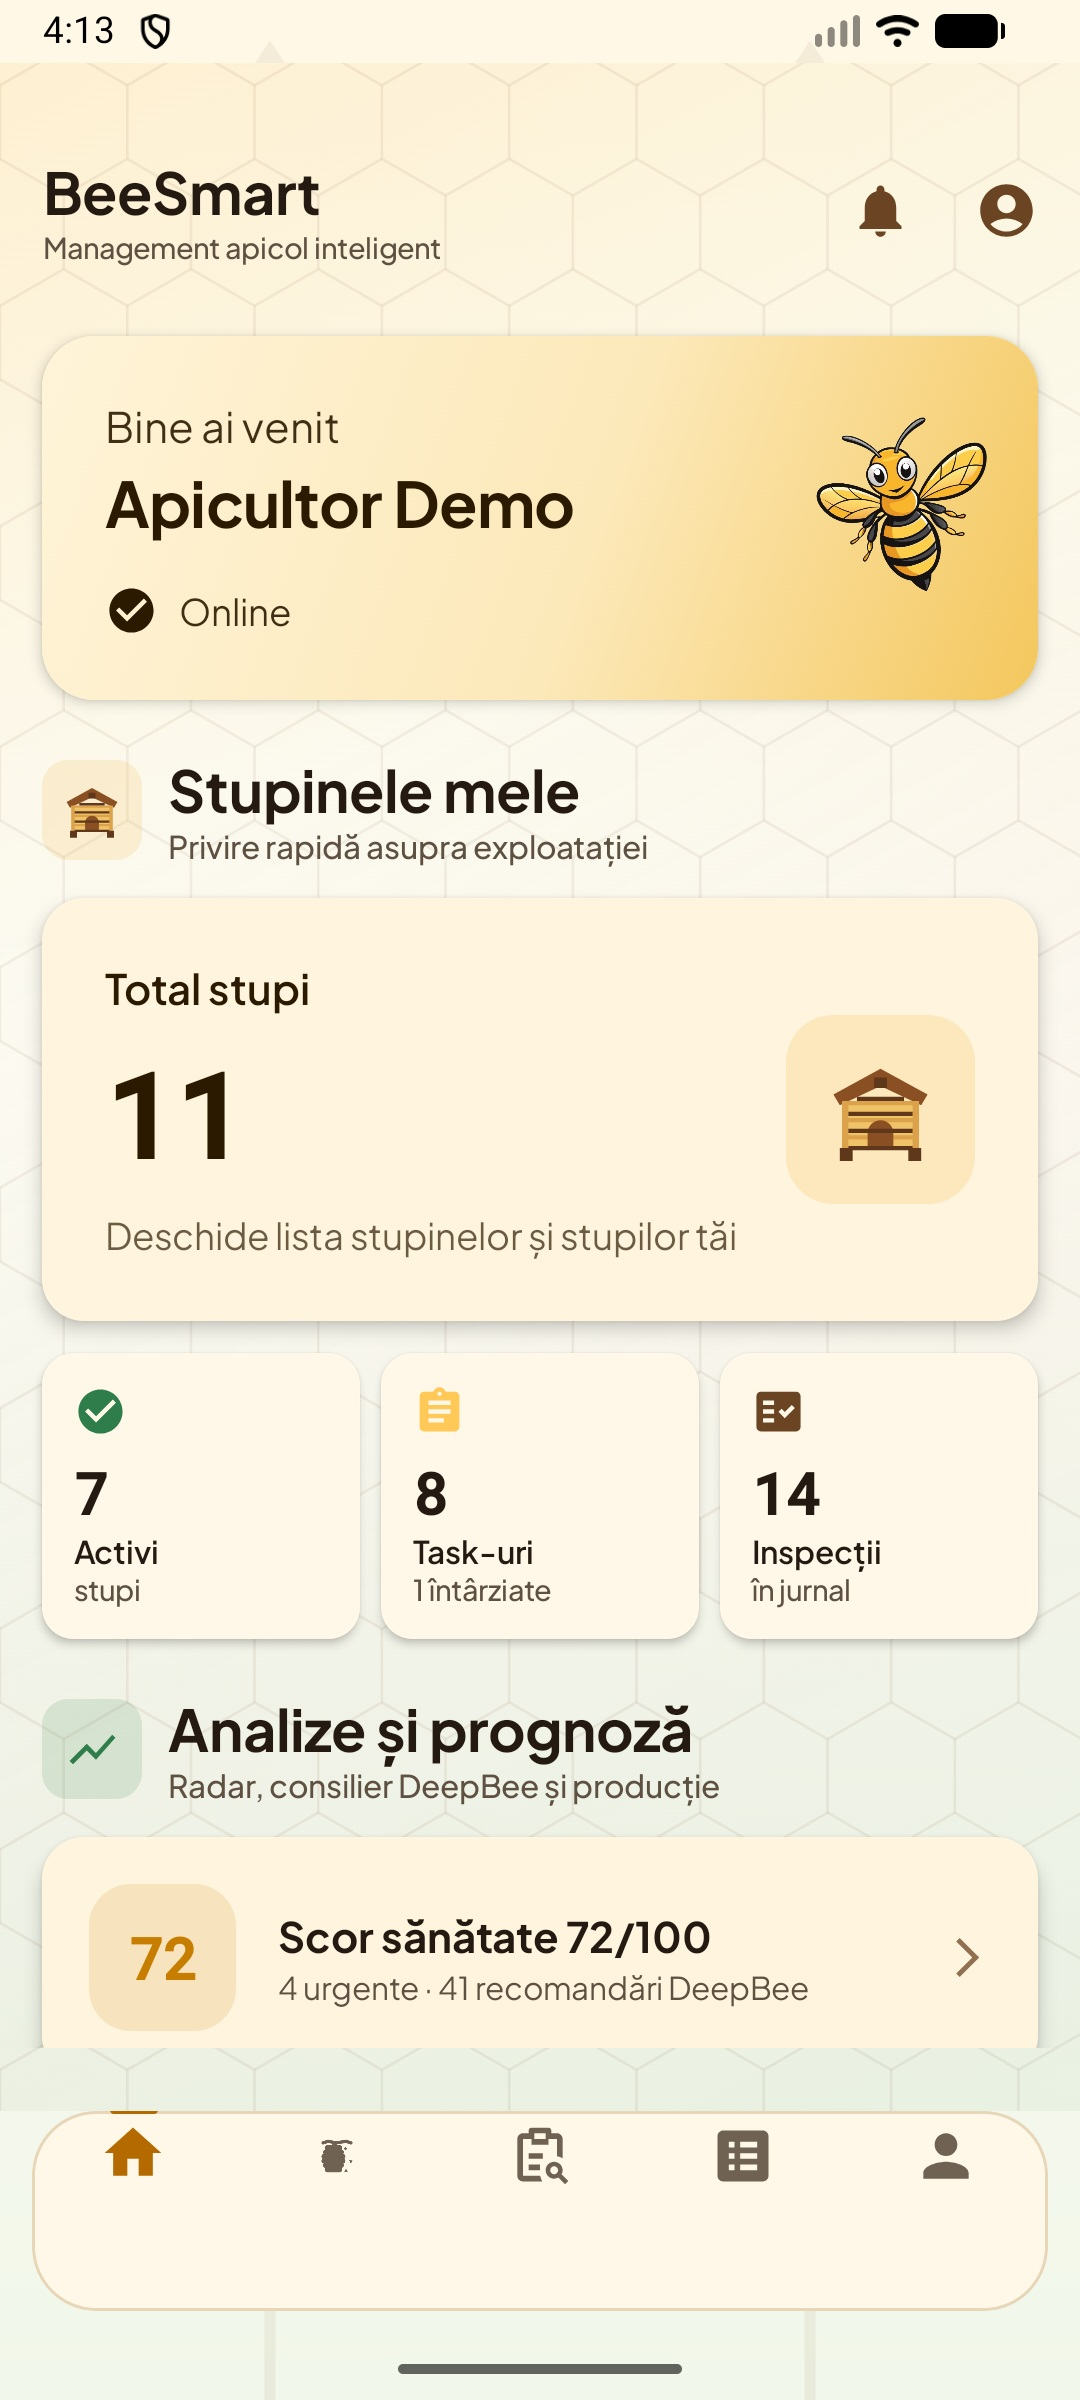
\includegraphics[width=0.40\textwidth]{./images/screenshots/04-dashboard-updated.jpg}}
	\hfill
	\subfigure[Acces rapid la module]{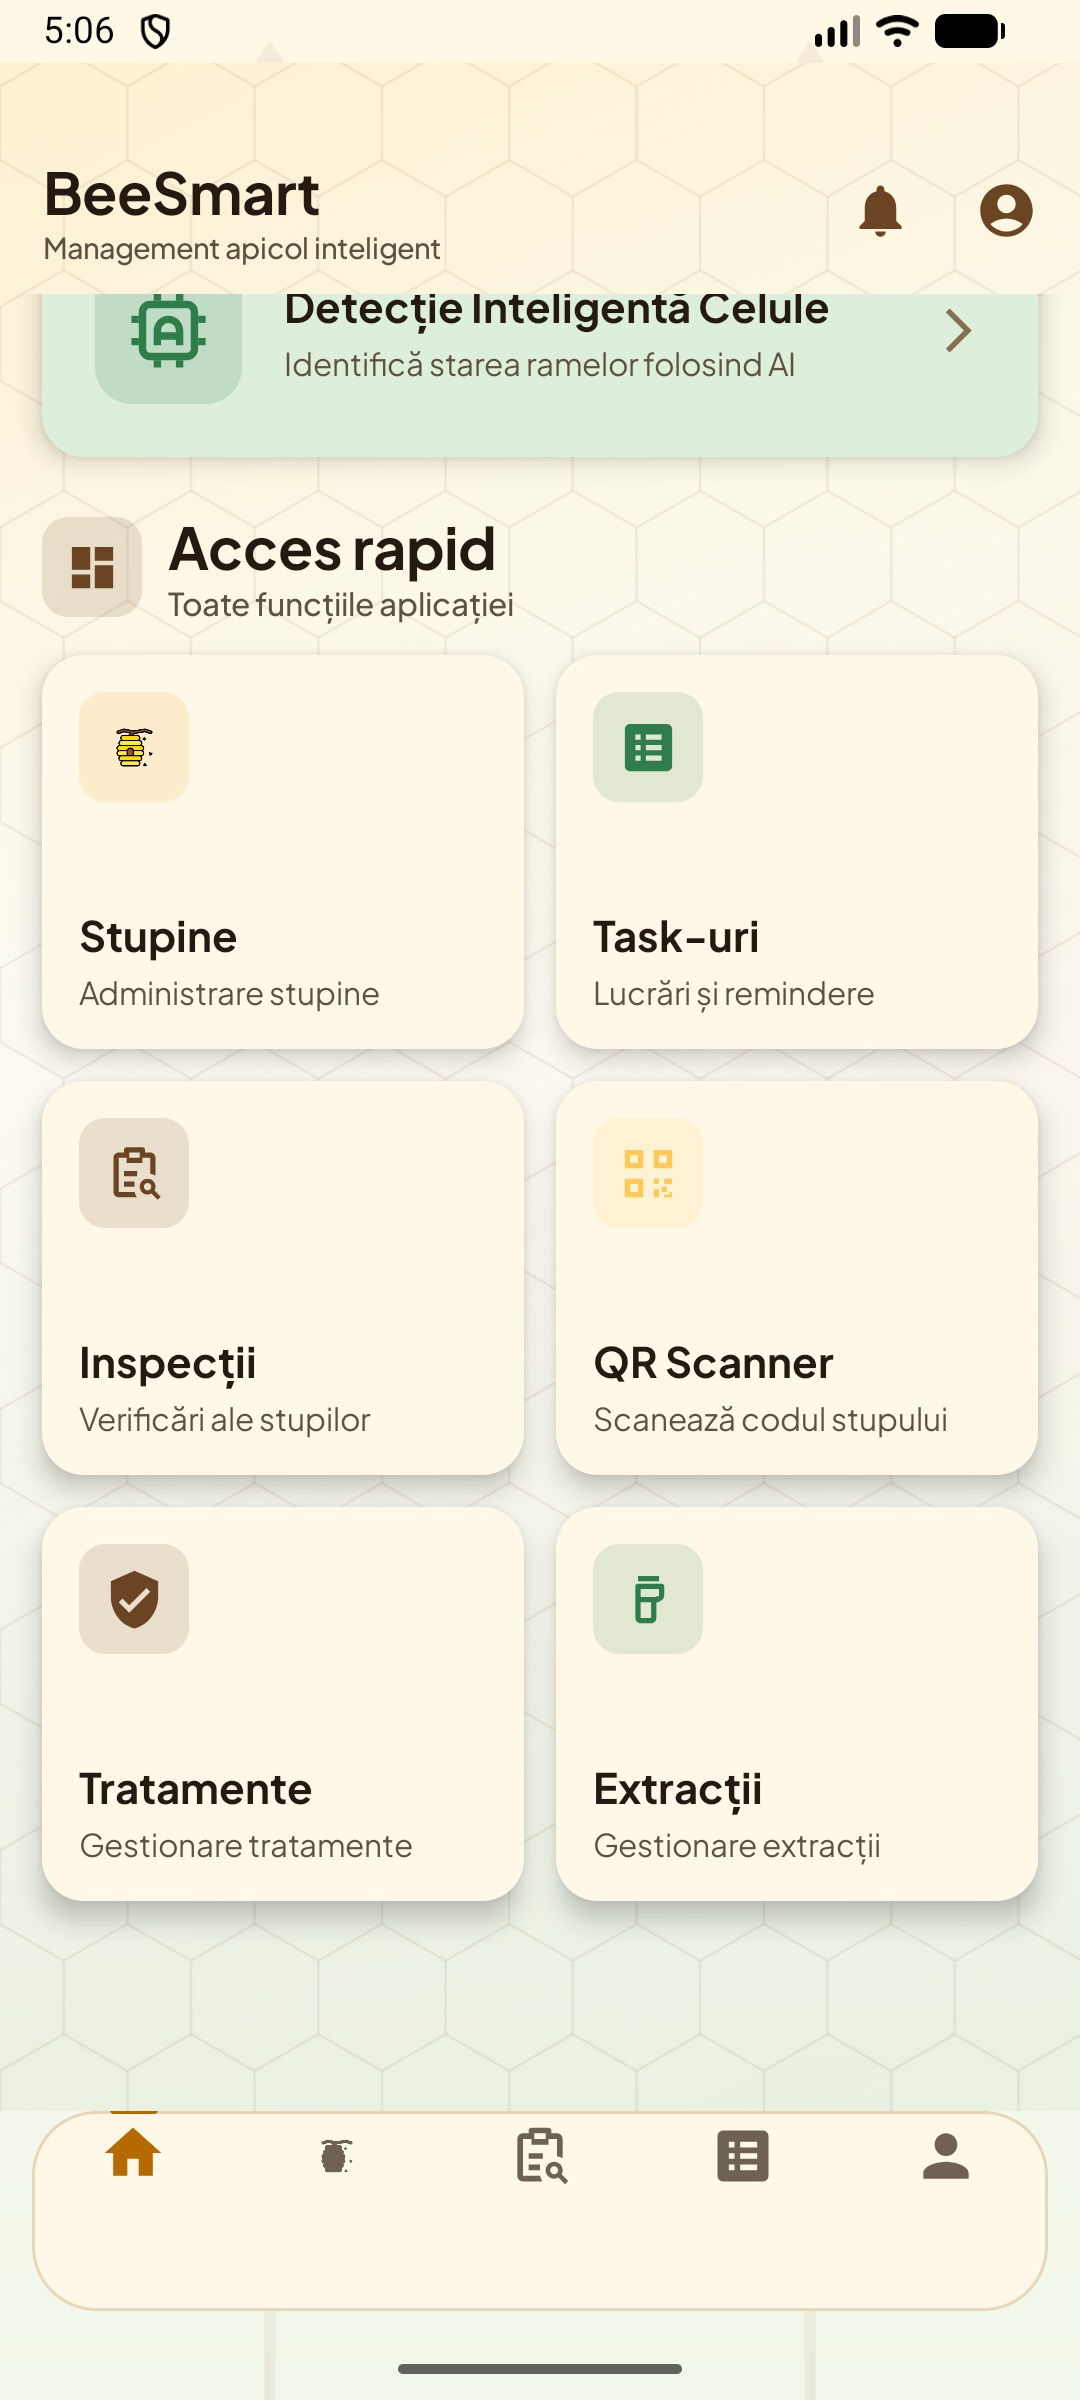
\includegraphics[width=0.40\textwidth]{./images/screenshots/home-modules-updated.jpg}}
	\caption{Ecranul principal al aplicației: partea de sumar a stupinei și zona de acces rapid la modulele de lucru.}
	\label{fig:home}
\end{figure}

\section{Scenariul de autentificare}

Primul scenariu este crearea unui cont și autentificarea. Utilizatorul accesează fluxul de register, introduce datele necesare, iar backend-ul creează contul, salvează parola hash-uită și generează token-urile necesare. În funcție de configurarea email, utilizatorul poate primi un link de confirmare. Linkul poate deschide aplicația prin schema \texttt{beesmart://confirm-email} sau prin domeniul \texttt{https://app.beesmart.ro/confirm-email}.

La login, aplicația primește un access token și un refresh token. Access token-ul este folosit pentru cererile protejate, iar refresh token-ul permite obținerea unui token nou fără reautentificare. \texttt{AuthInterceptor} tratează expirarea token-ului și reia cererea cu token-ul nou, atunci când refresh-ul reușește. Dacă refresh-ul eșuează, sesiunea este curățată și utilizatorul trebuie să se autentifice din nou. Ecranele de autentificare și de înregistrare sunt prezentate în figura~\ref{fig:auth}.

\begin{figure}[H]
	\centering
	\subfigure[Autentificare]{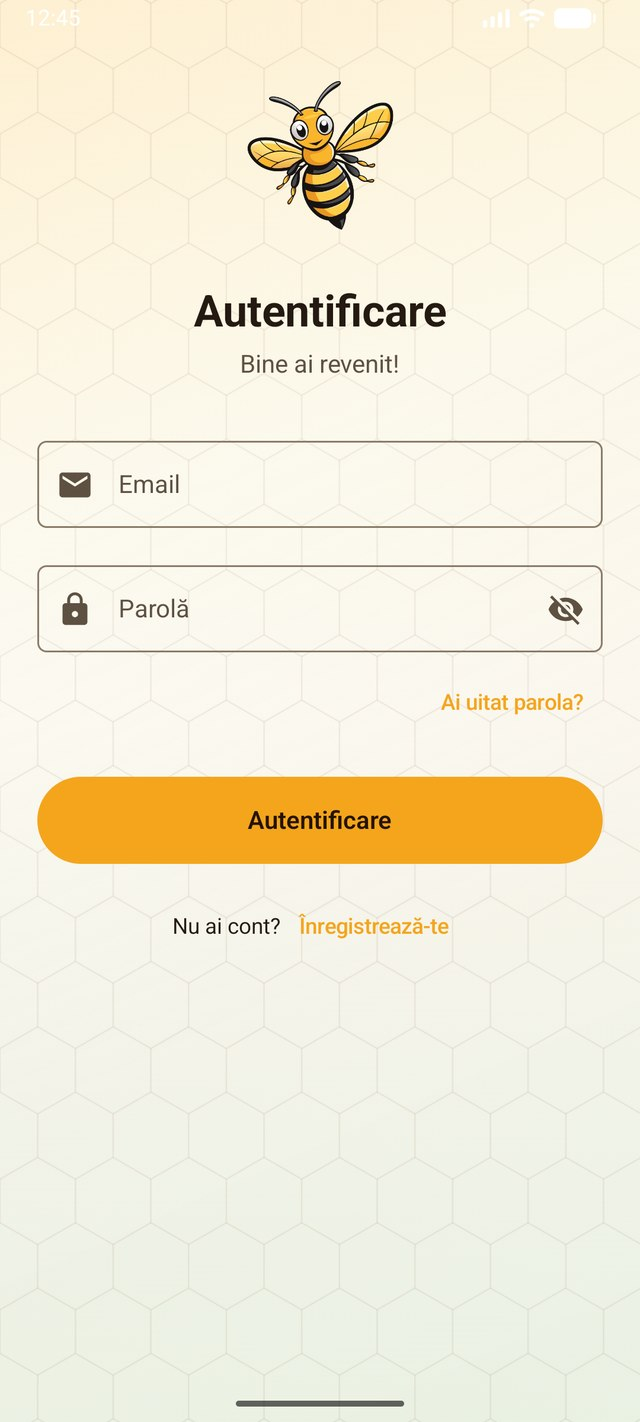
\includegraphics[width=0.40\textwidth]{./images/screenshots/01-login.jpg}}
	\hfill
	\subfigure[Înregistrare cont nou]{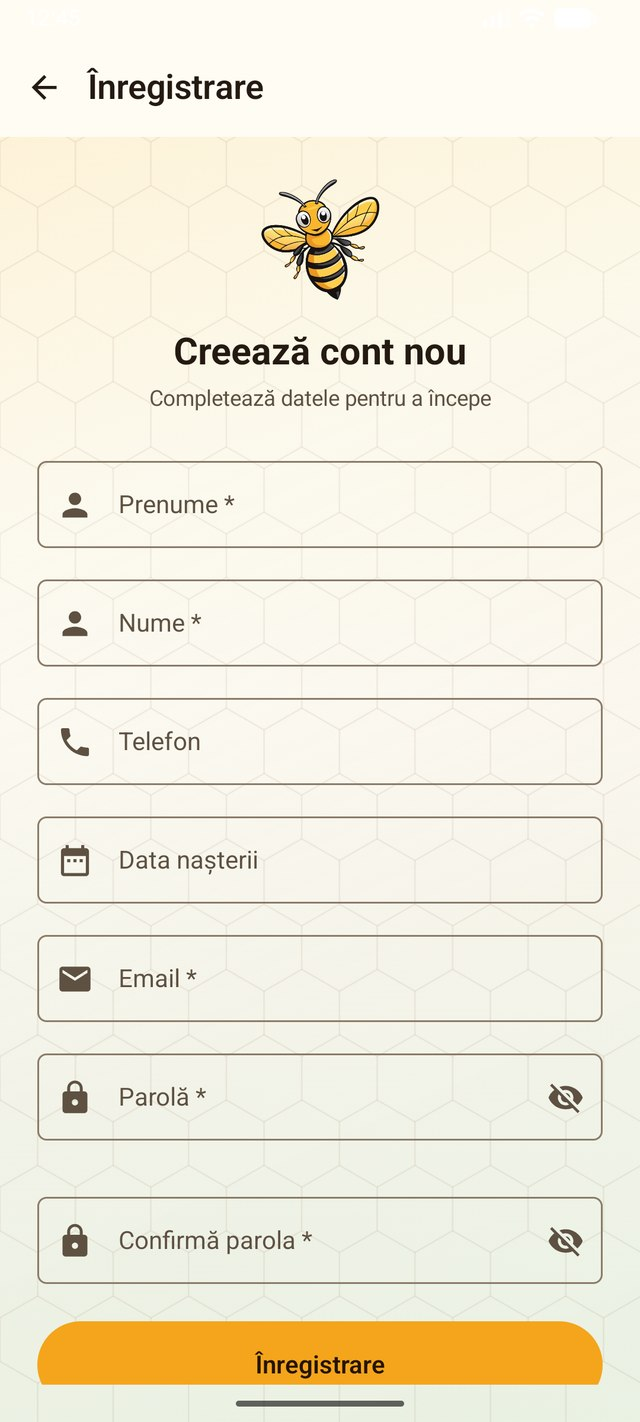
\includegraphics[width=0.40\textwidth]{./images/screenshots/02-register-empty.jpg}}
	\caption{Fluxul de autentificare: ecranul de login și formularul de înregistrare.}
	\label{fig:auth}
\end{figure}

\section{Crearea unei stupine}

După autentificare, utilizatorul poate crea o stupină. Formularul conține nume, descriere și locație. Locația este importantă nu doar ca informație descriptivă, ci și pentru integrarea meteo. \texttt{WeatherRepository} folosește textul locației pentru geocodare și apoi pentru obținerea datelor de vreme curentă.

Dacă utilizatorul creează stupina fără internet, aplicația generează un id local, salvează \texttt{ApiaryEntity} în Room și adaugă operația în \texttt{sync\_queue}. În listă, stupina apare imediat, chiar dacă serverul nu a confirmat-o încă. Când conexiunea revine, \texttt{SyncManager} trimite cererea către backend, primește id-ul de server și actualizează rândul local. Formularul de creare a unei stupine este ilustrat în figura~\ref{fig:create-apiary}.

\begin{figure}[H]
	\centering
	\subfigure[Formular gol]{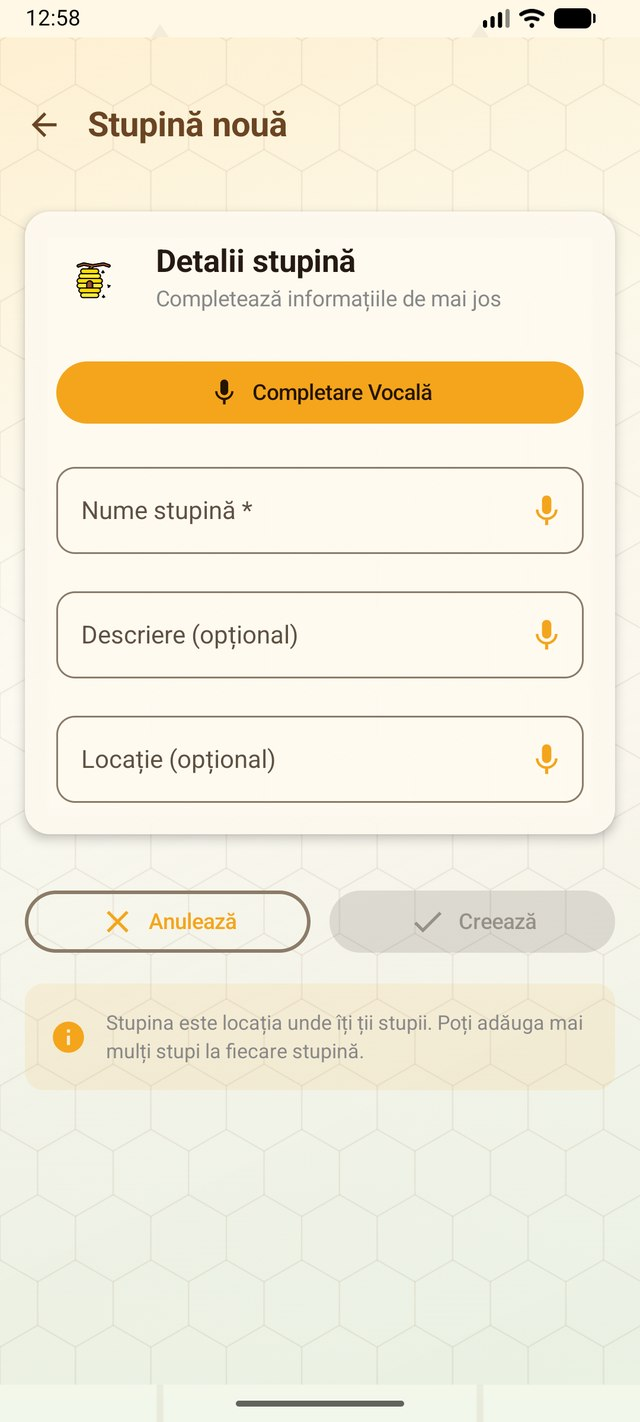
\includegraphics[width=0.40\textwidth]{./images/screenshots/06-create-apiary-form.jpg}}
	\hfill
	\subfigure[Formular completat]{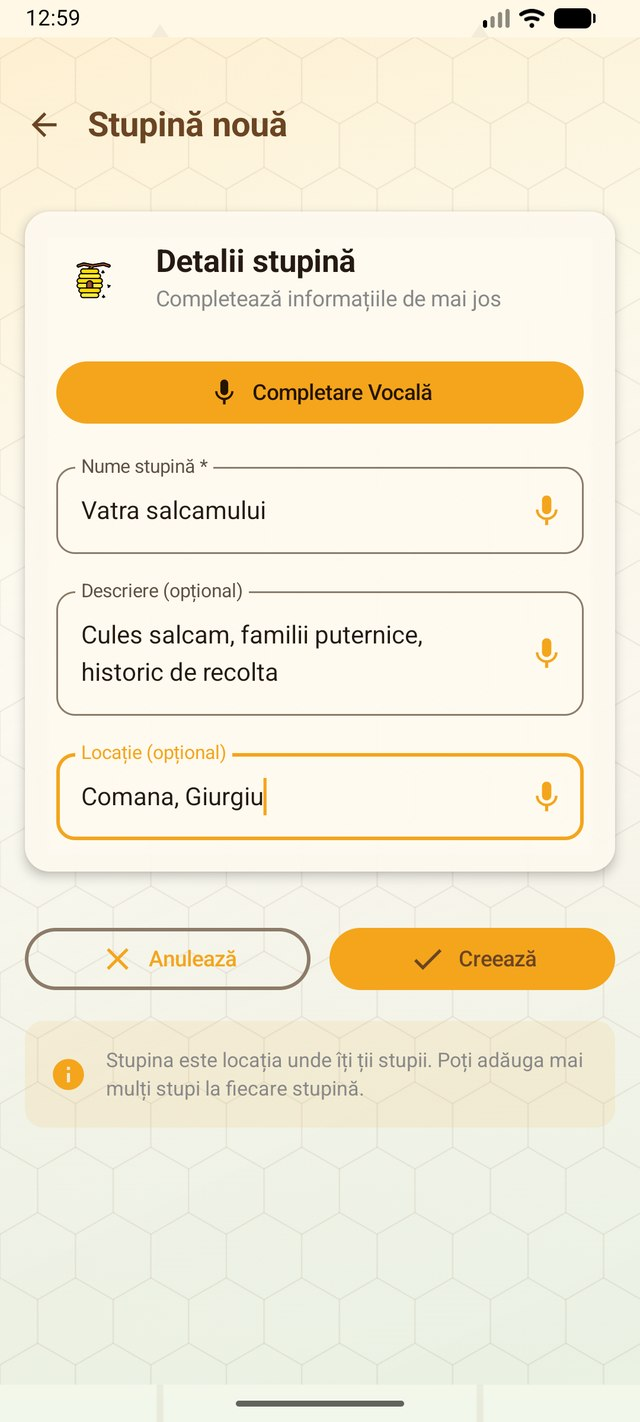
\includegraphics[width=0.40\textwidth]{./images/screenshots/07-create-apiary-filled.jpg}}
	\caption{Crearea unei stupine: formularul cu nume, descriere și locație, cu opțiunea de completare vocală.}
	\label{fig:create-apiary}
\end{figure}

\section{Adăugarea și gestionarea stupilor}

În interiorul unei stupine, utilizatorul poate adăuga stupi. Modelul \texttt{Hive} conține câmpuri precum nume, tip, status, note, prezența mătcii, vârsta mătcii, rame cu albine, rame cu puiet, rame cu miere și ultima inspecție. Aceste câmpuri permit o descriere rapidă a stării generale a stupului, fără a intra neapărat în istoricul complet al inspecțiilor.

Stupii pot fi creați și offline. Dacă stupina părinte nu a fost încă sincronizată, \texttt{SyncManager} amână crearea stupului până când stupina primește \texttt{serverId}. Această logică este importantă deoarece backend-ul cere id-ul real al stupinei pentru ruta de creare a stupului.

Fiecare stup poate avea un cod QR generat din linkul de deep link. Codul poate fi salvat ca imagine, distribuit sau exportat într-un PDF simplu. În teren, scanarea codului QR permite deschiderea rapidă a fișei stupului, fără căutare manuală în listă. Lista stupilor, formularul de adăugare și codul QR generat sunt prezentate în figura~\ref{fig:hives}.

\begin{figure}[H]
	\centering
	\subfigure[Lista stupilor cu statusuri]{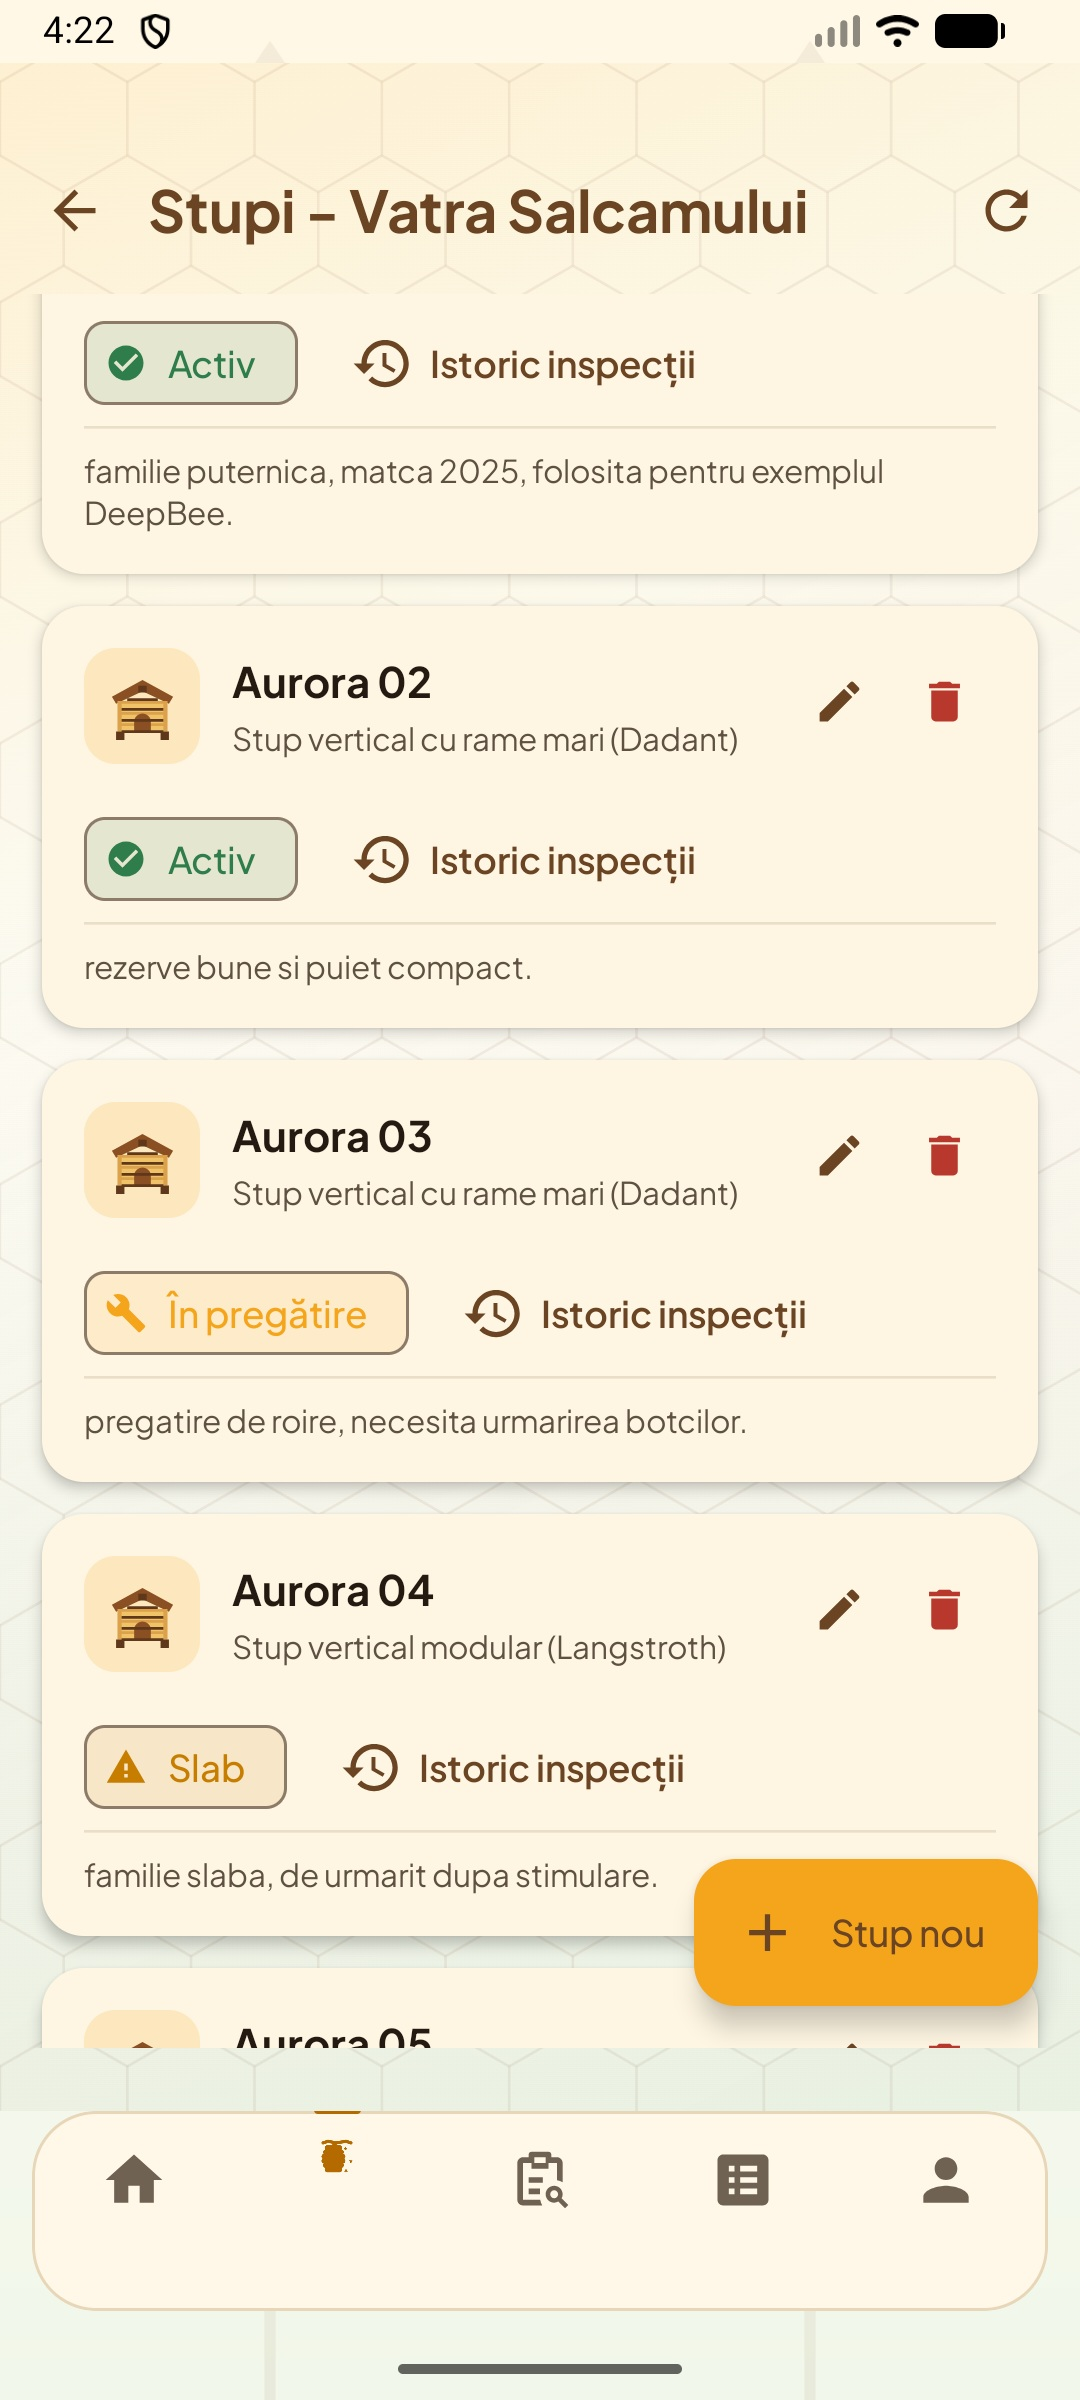
\includegraphics[width=0.30\textwidth]{./images/screenshots/16-vatra-hives-risk-list-updated.jpg}}
	\hfill
	\subfigure[Formular de adăugare stup]{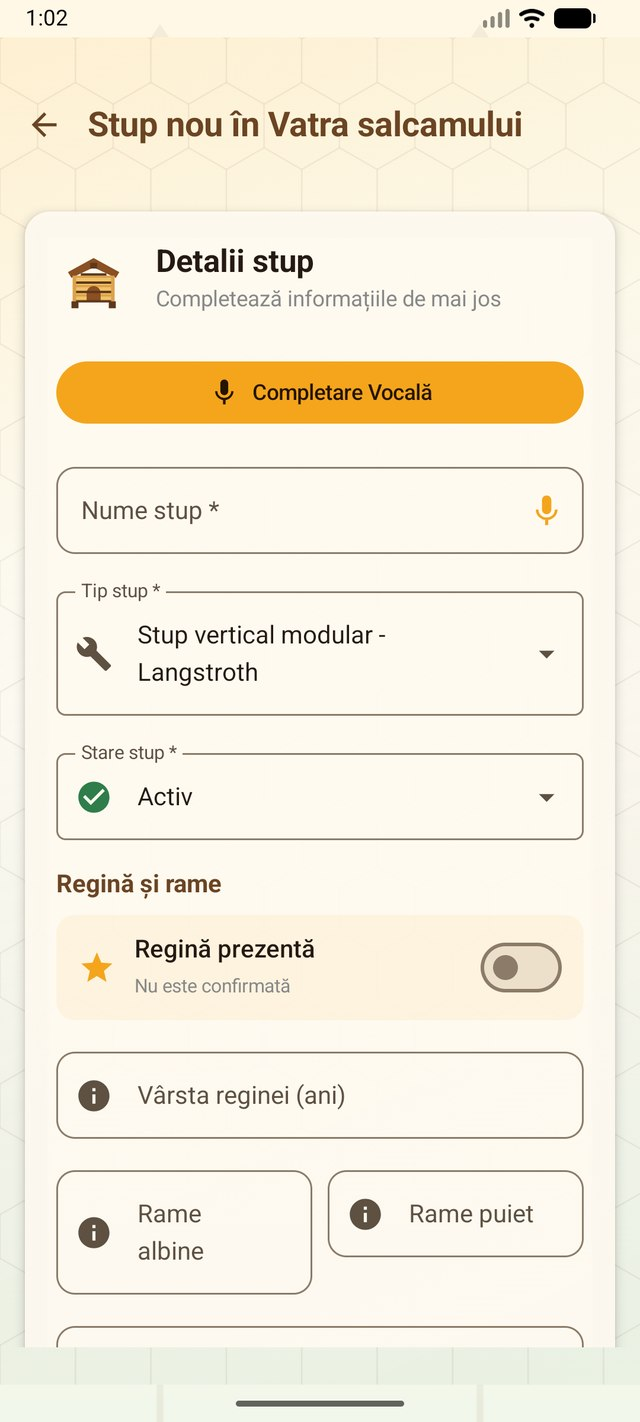
\includegraphics[width=0.30\textwidth]{./images/screenshots/10-create-hive-form.jpg}}
	\hfill
	\subfigure[Cod QR al stupului]{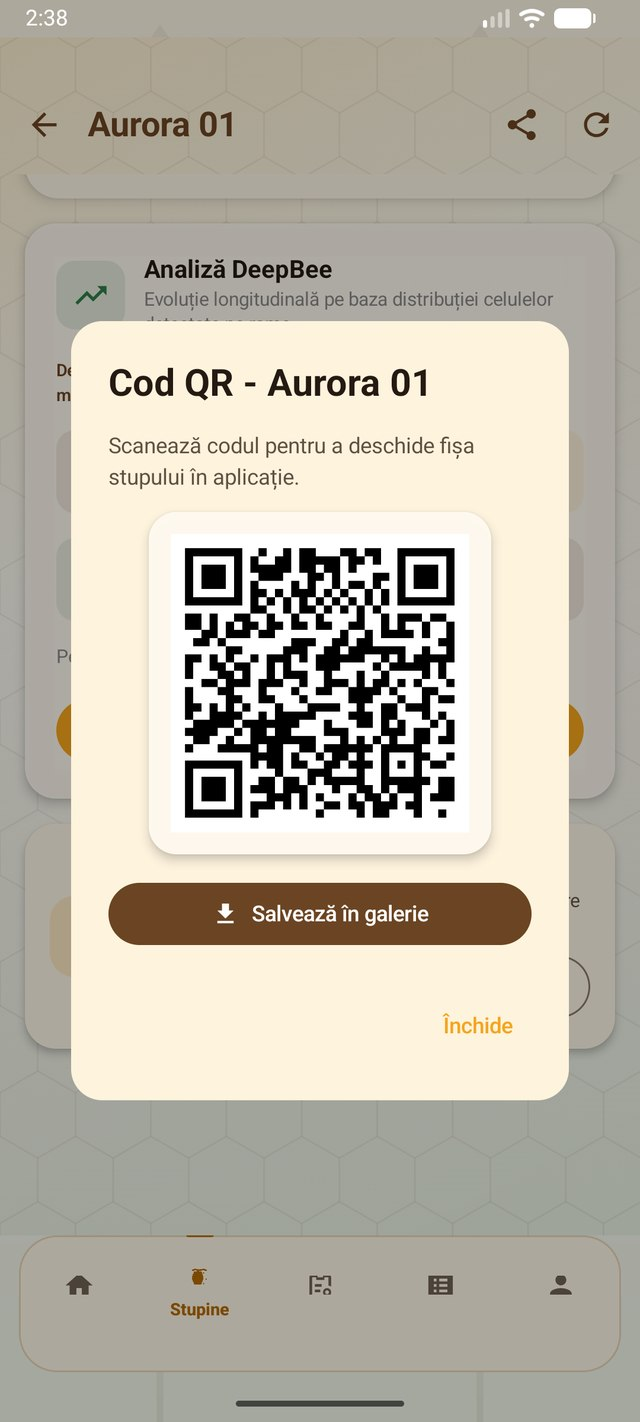
\includegraphics[width=0.30\textwidth]{./images/screenshots/hive-qr.jpg}}
	\caption{Gestionarea stupilor: lista cu statusuri (activ, slab, fără regină), formularul de creare și codul QR generat pentru deschiderea rapidă a fișei.}
	\label{fig:hives}
\end{figure}

\section{Realizarea unei inspecții}

Inspecția este scenariul cel mai complex din aplicație. Utilizatorul selectează stupul, data inspecției, temperatura și completează valori despre rame: număr total, rame cu puiet, rame cu miere și rame cu polen. Câmpurile de bază includ și prezența mătcii, a ouălor și a larvelor.

\begin{figure}[H]
	\centering
	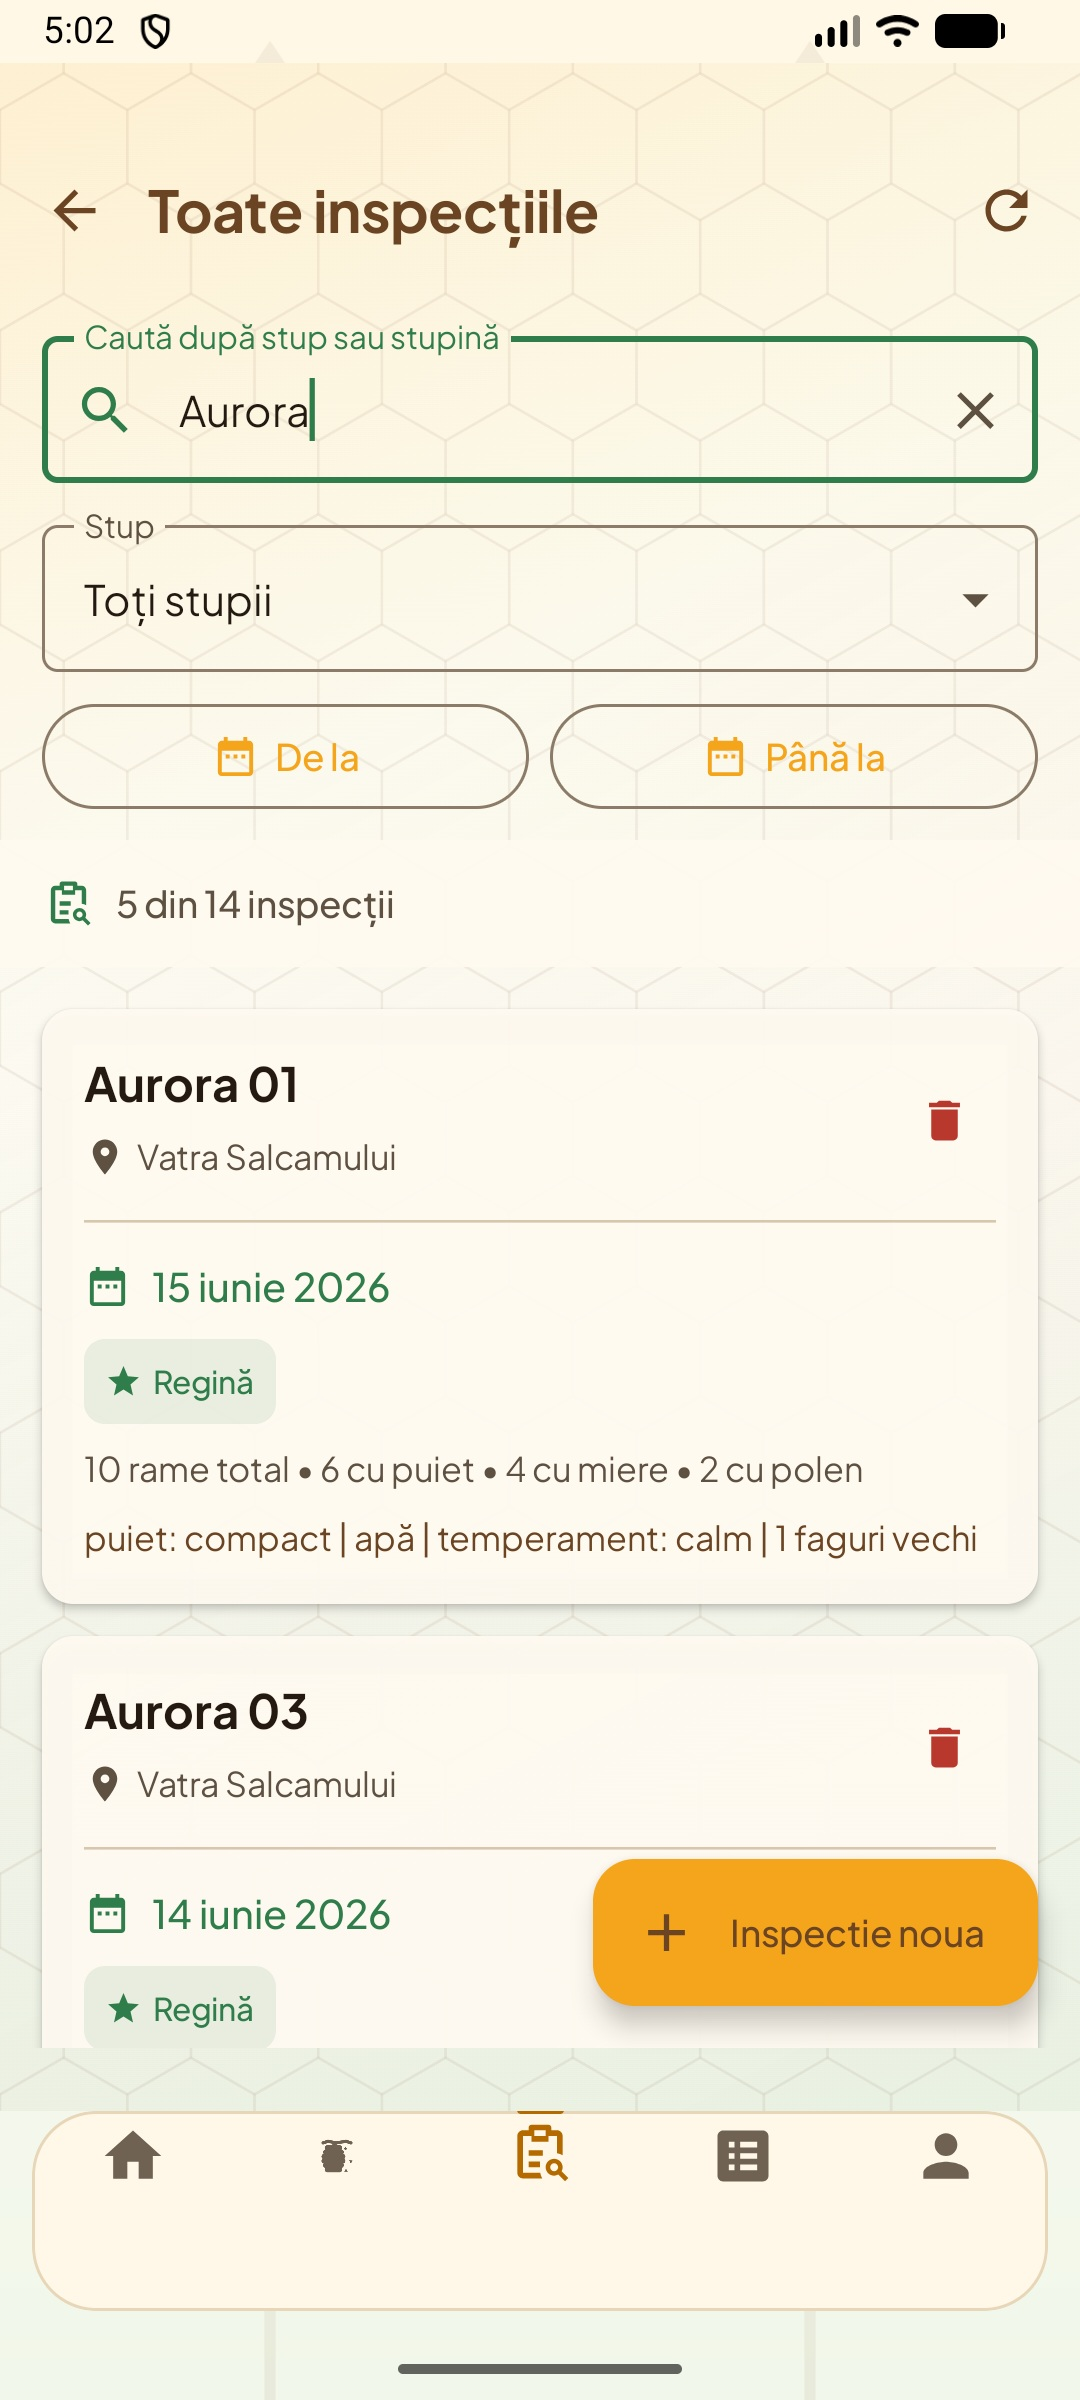
\includegraphics[width=0.40\textwidth]{./images/screenshots/inspection-list-updated.jpg}
	\caption{Jurnalul de inspecții actualizat: utilizatorul poate căuta după stup sau stupină, poate filtra după stup și perioadă și poate vedea rapid indicatorii principali ai fiecărei verificări.}
	\label{fig:inspection-list}
\end{figure}

Formularul a fost extins cu 13 câmpuri suplimentare care permit capturarea unui context mai complet al stării familiei. Utilizatorul poate marca botcile observate, botcile cu ouă (semnal direct de pregătire a roirii), aglomerarea sau barba la urdiniș, spațiul insuficient în stup, tiparele de puiet (compact, dispersat etc.), procentul mierii căpăcite, hrănirea efectuată în ziua inspecției, disponibilitatea apei, prezența umidității sau mucegaiului, albinele moarte la urdiniș, comportamentul neobișnuit al coloniei, temperamentul acesteia și numărul de faguri vechi care trebuie înlocuiți. Aceste date sunt salvate în aceeași entitate de inspecție, atât local, cât și pe server, și sunt folosite ulterior de advisorul contextual pentru generarea sfaturilor.


Formularul permite adăugarea de fotografii. Fotografiile pot fi realizate cu camera sau selectate din galerie, apoi sunt procesate de \texttt{PhotoManager}. În fluxul actual, fotografia este transformată în Base64 și trimisă ca Data URI. Dacă inspecția este salvată offline, fotografiile sunt memorate local și sincronizate după ce inspecția părinte primește id de server.

Utilizatorul poate rula analiza AI pentru o fotografie individuală, pentru fotografiile selectate sau pentru toate fotografiile atașate inspecției. Dacă backend-ul este disponibil, imaginea este trimisă la endpoint-ul \texttt{analyze-cells}. Rezultatul este afișat în dialogul de previzualizare al fotografiei, unde utilizatorul vede numărul de celule detectate, câte au coordonate, nivelul de încredere și raportul orientativ generat de \texttt{BroodAnalyzer}. Răspunsul poate fi:
\begin{itemize}
	\item \texttt{success}, dacă analiza a reușit;
	\item \texttt{low\_quality}, dacă fotografia este prea mică, neclară, prea întunecată, supraexpusă sau cu contrast insuficient;
	\item \texttt{not\_comb\_image}, dacă nu se detectează suficiente celule de fagure;
	\item \texttt{uncertain\_analysis}, dacă modelul are încredere scăzută în prea multe celule.
\end{itemize}

După succes, \texttt{BroodAnalyzer} transformă rezultatele în raport. Raportul poate evidenția semnale pozitive, precum prezența simultană a ouălor, larvelor și puietului căpăcit, sau semnale de atenție, precum lipsa larvelor ori rezerve scăzute. Aceste mesaje sunt orientative și trebuie interpretate împreună cu observația apicultorului. Rezultatul analizei DeepBee, așa cum este afișat în aplicație, este prezentat în figura~\ref{fig:ai-result}.

\begin{figure}[H]
	\centering
	\subfigure[Rezumatul analizei pe fotografie]{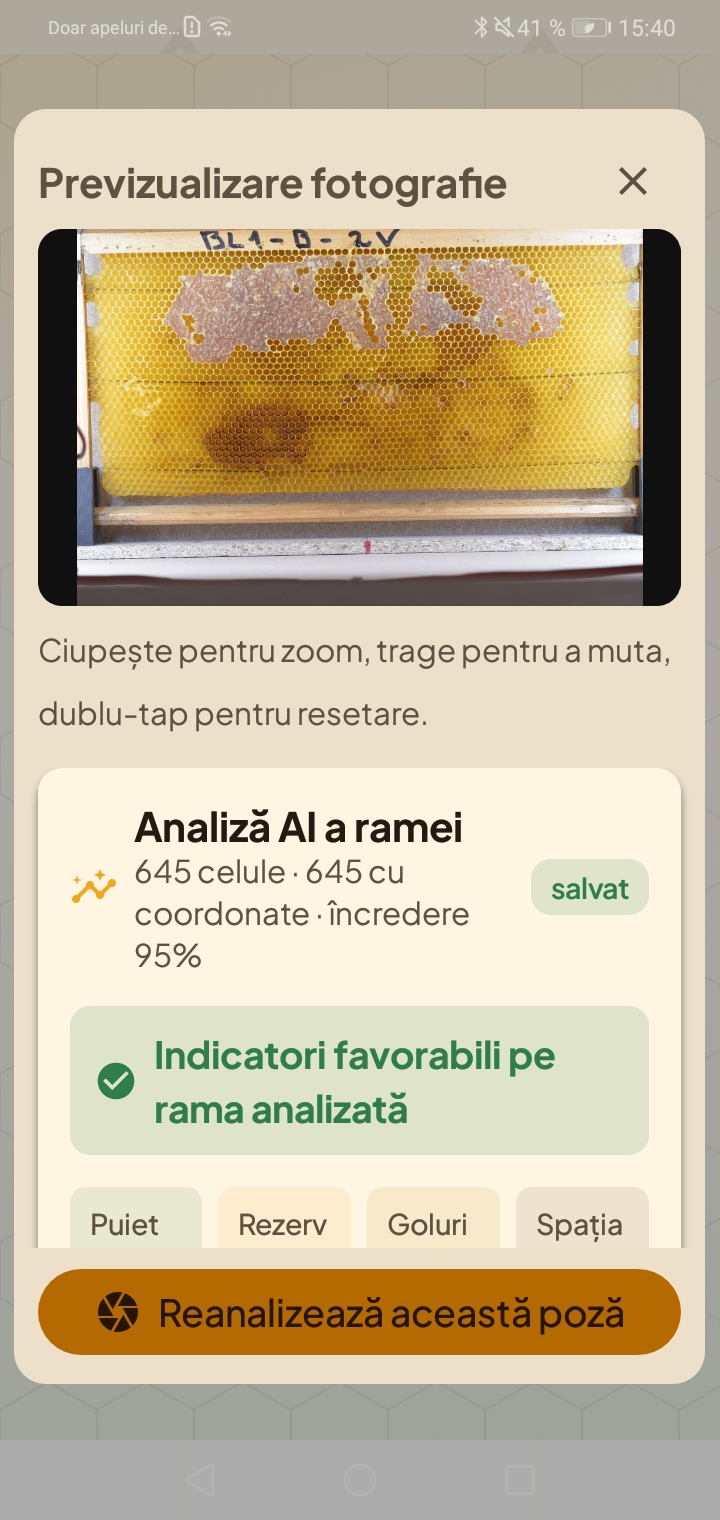
\includegraphics[width=0.40\textwidth]{./images/screenshots/ai-photo-preview-summary.jpg}}
	\hfill
	\subfigure[Detalii și pași recomandați]{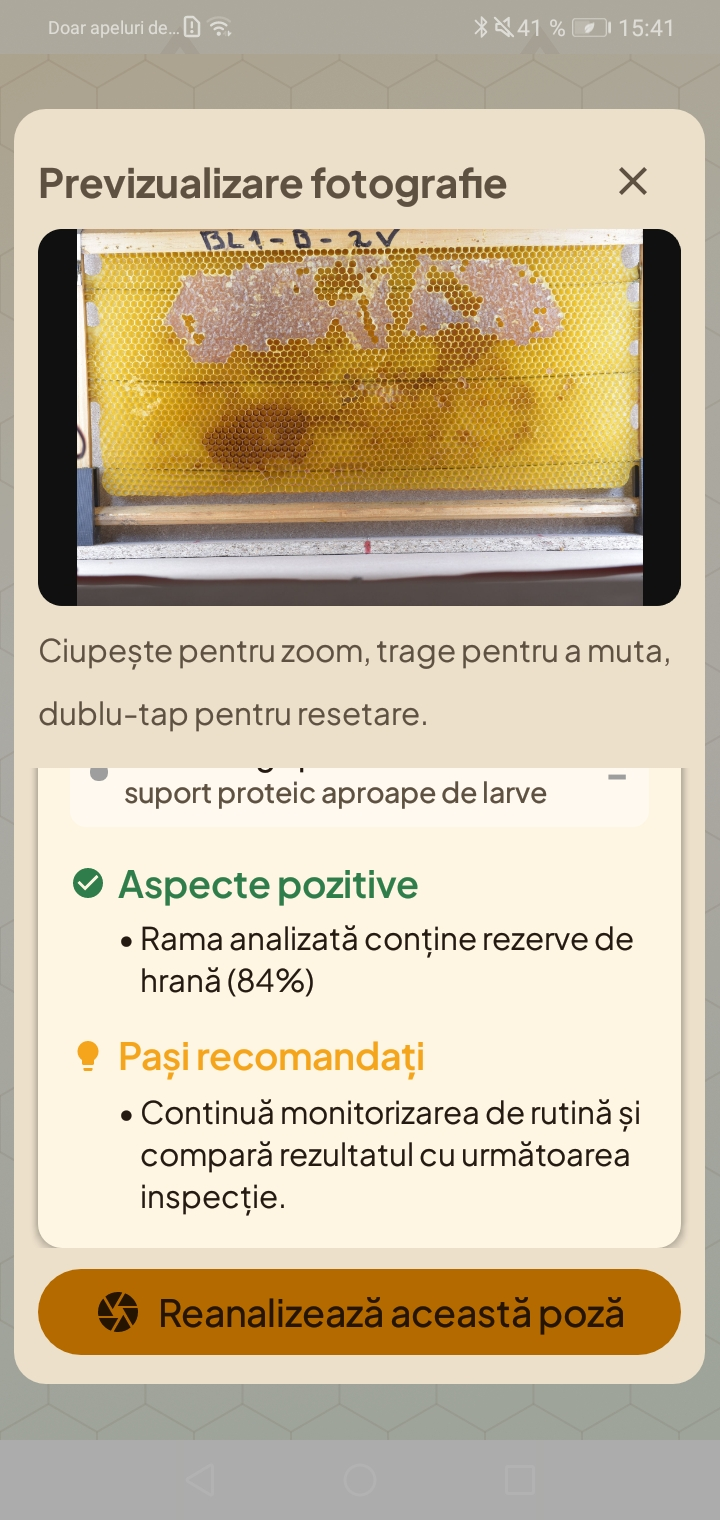
\includegraphics[width=0.40\textwidth]{./images/screenshots/ai-photo-preview-details.jpg}}
	\caption{Previzualizarea fotografiei de ramă după analiza AI: aplicația afișează numărul de celule detectate, existența coordonatelor, încrederea medie, verdictul orientativ, aspectele pozitive și pașii recomandați.}
	\label{fig:ai-result}
\end{figure}

\section{Vizualizarea statisticilor pe stup}

Pentru fiecare stup, aplicația poate afișa un raport DeepBee longitudinal. Ecranul \texttt{HiveStatsScreen} pornește de la analizele AI salvate și calculează puncte de sănătate pe luni. Utilizatorul vede numărul de celule analizate, indexul curent, puietul, rezervele și tendința față de analiza precedentă.

Ecranul include două tipuri de vizualizare:
\begin{itemize}
	\item evoluția lunară pentru anul curent, utilă pentru urmărirea sezonului;
	\item comparația inter-anuală pentru aceeași lună, utilă pentru observarea diferențelor de la un an la altul.
\end{itemize}

În plus, ultima analiză este detaliată prin distribuția celulelor și indicatori derivați. Această funcție transformă analiza AI dintr-un rezultat punctual într-un istoric utilizabil. Apicultorul nu vede doar \enquote{fotografia X a avut N celule}, ci poate observa dacă valorile se schimbă în timp. Raportul DeepBee longitudinal pe stup este ilustrat în figura~\ref{fig:hive-stats}.

\begin{figure}[H]
	\centering
	\subfigure[Indicatori longitudinali]{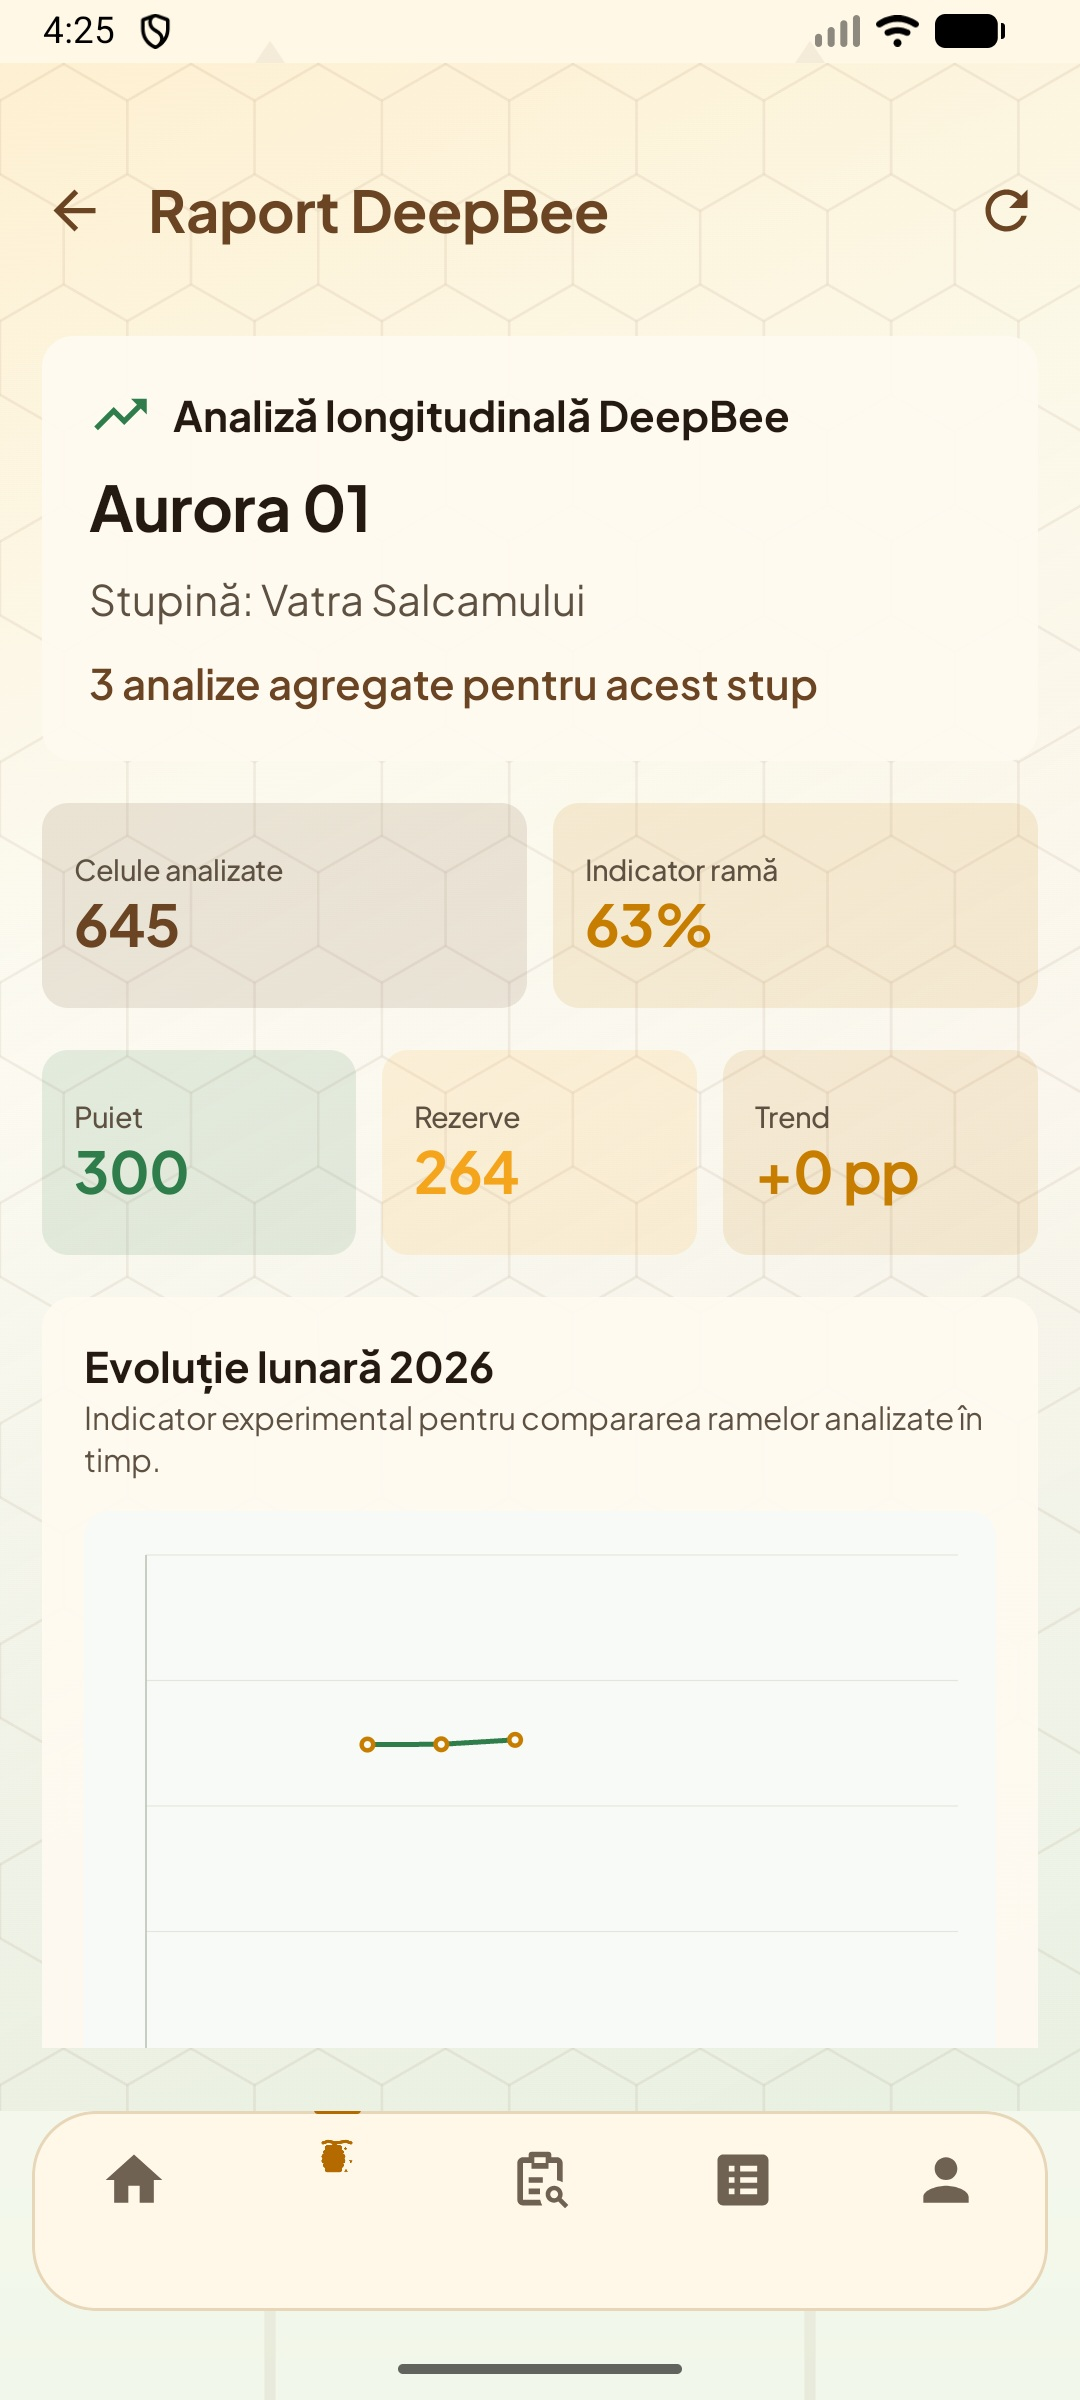
\includegraphics[width=0.40\textwidth]{./images/screenshots/hive-deepbee-stats-updated.jpg}}
	\hfill
	\subfigure[Distribuția ultimei analize]{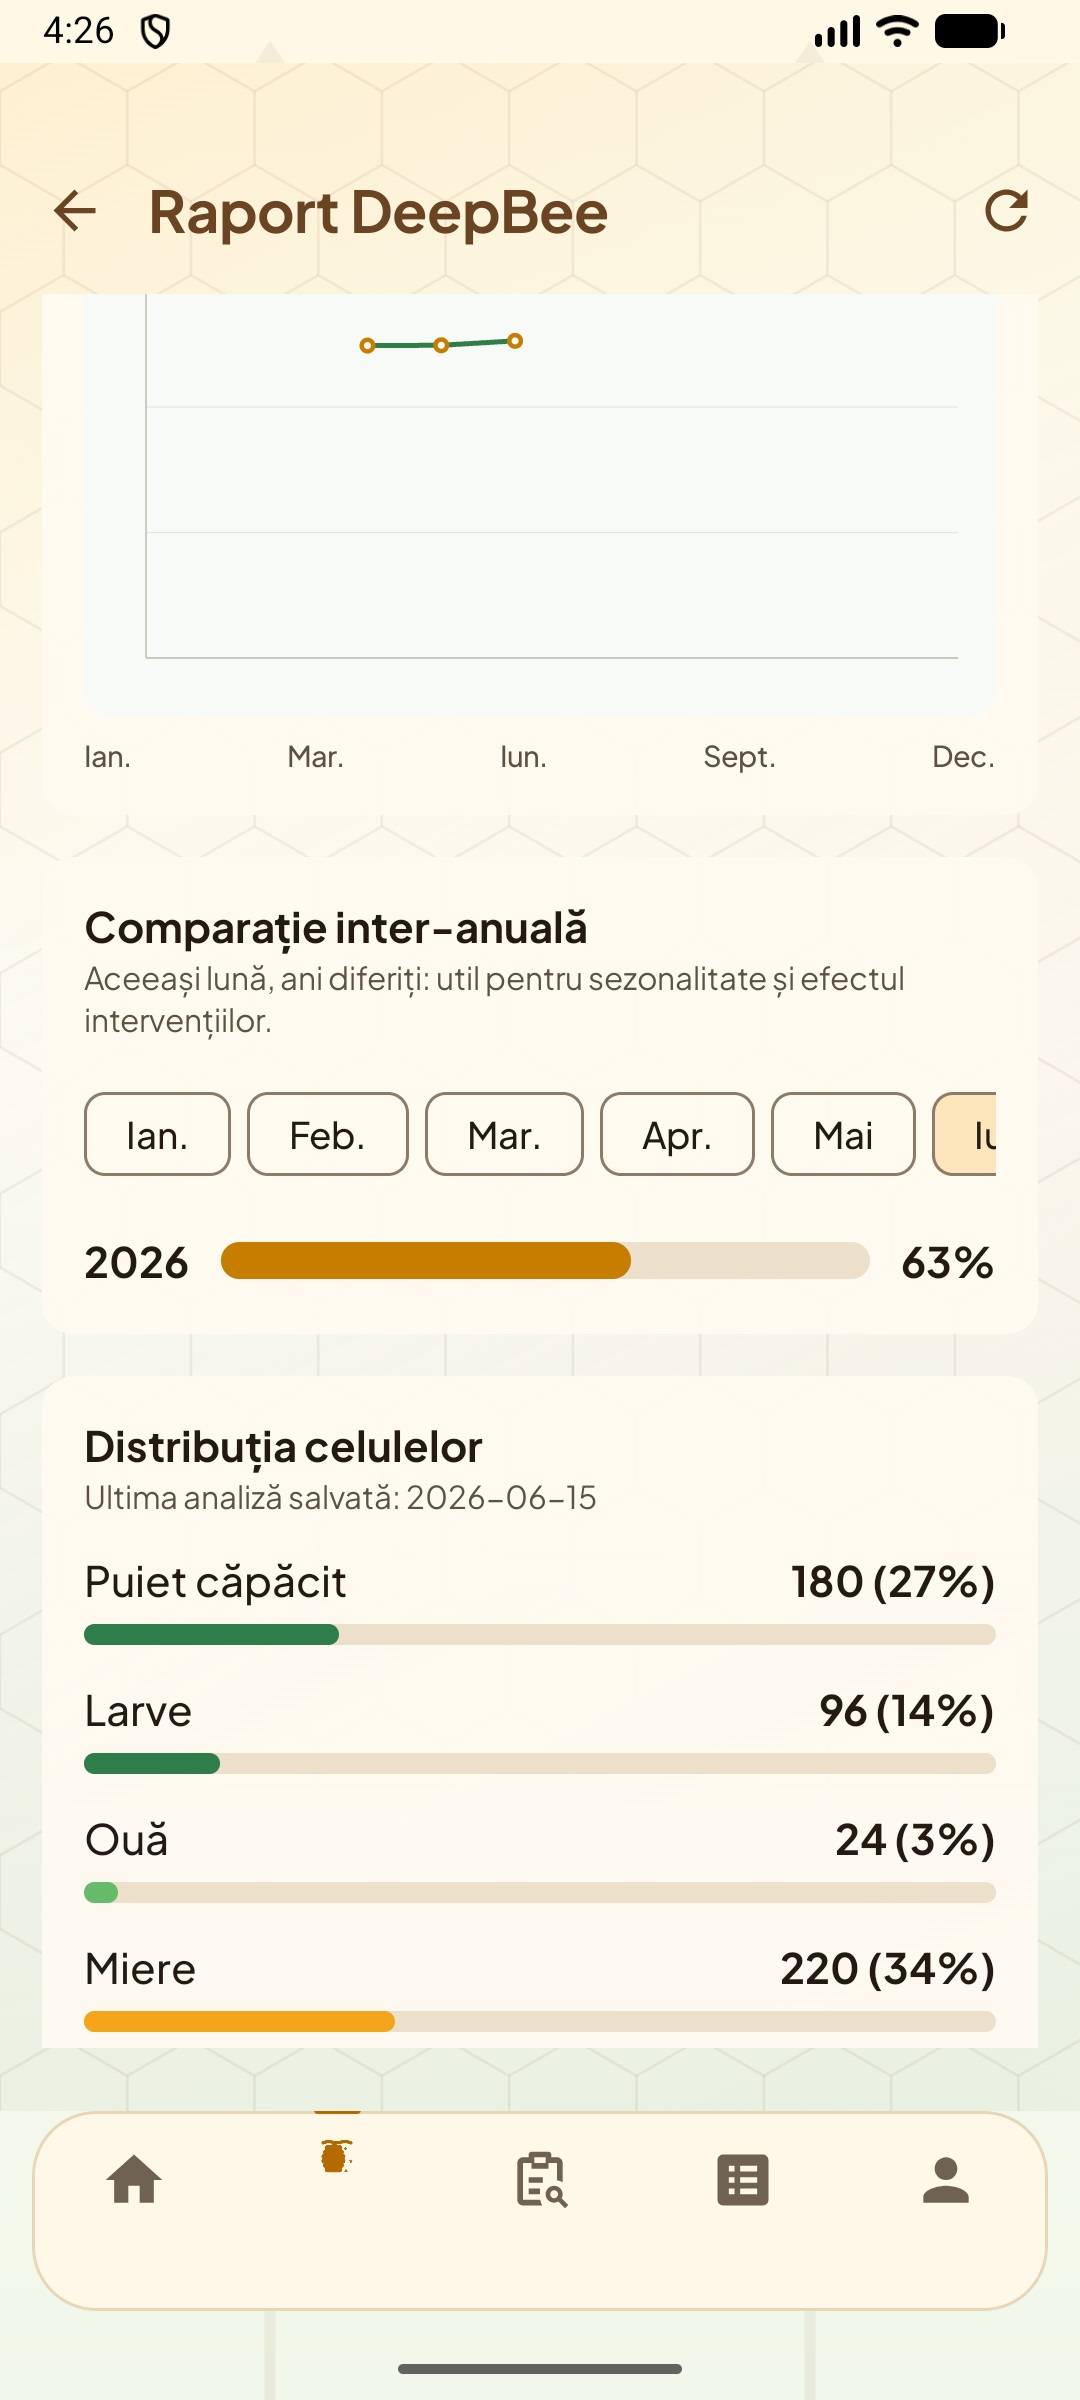
\includegraphics[width=0.40\textwidth]{./images/screenshots/hive-deepbee-distribution-updated.jpg}}
	\caption{Raportul DeepBee longitudinal pentru un stup: numărul de analize agregate, celulele analizate, indicatorul ramei, trendul lunar și distribuția pe categorii pentru ultima fotografie analizată.}
	\label{fig:hive-stats}
\end{figure}

\section{Dashboard cu analytics la nivel de stupină}

Ecranul principal al aplicației include un set de carduri cu indicatori calculați la nivel de stupină, actualizați la fiecare încărcare a ecranului. Aceste date sunt produse local de \texttt{DashboardAnalyticsCalculator} și nu necesită un apel suplimentar la server.

\begin{figure}[H]
	\centering
	\subfigure[Index de sănătate și plan recomandat]{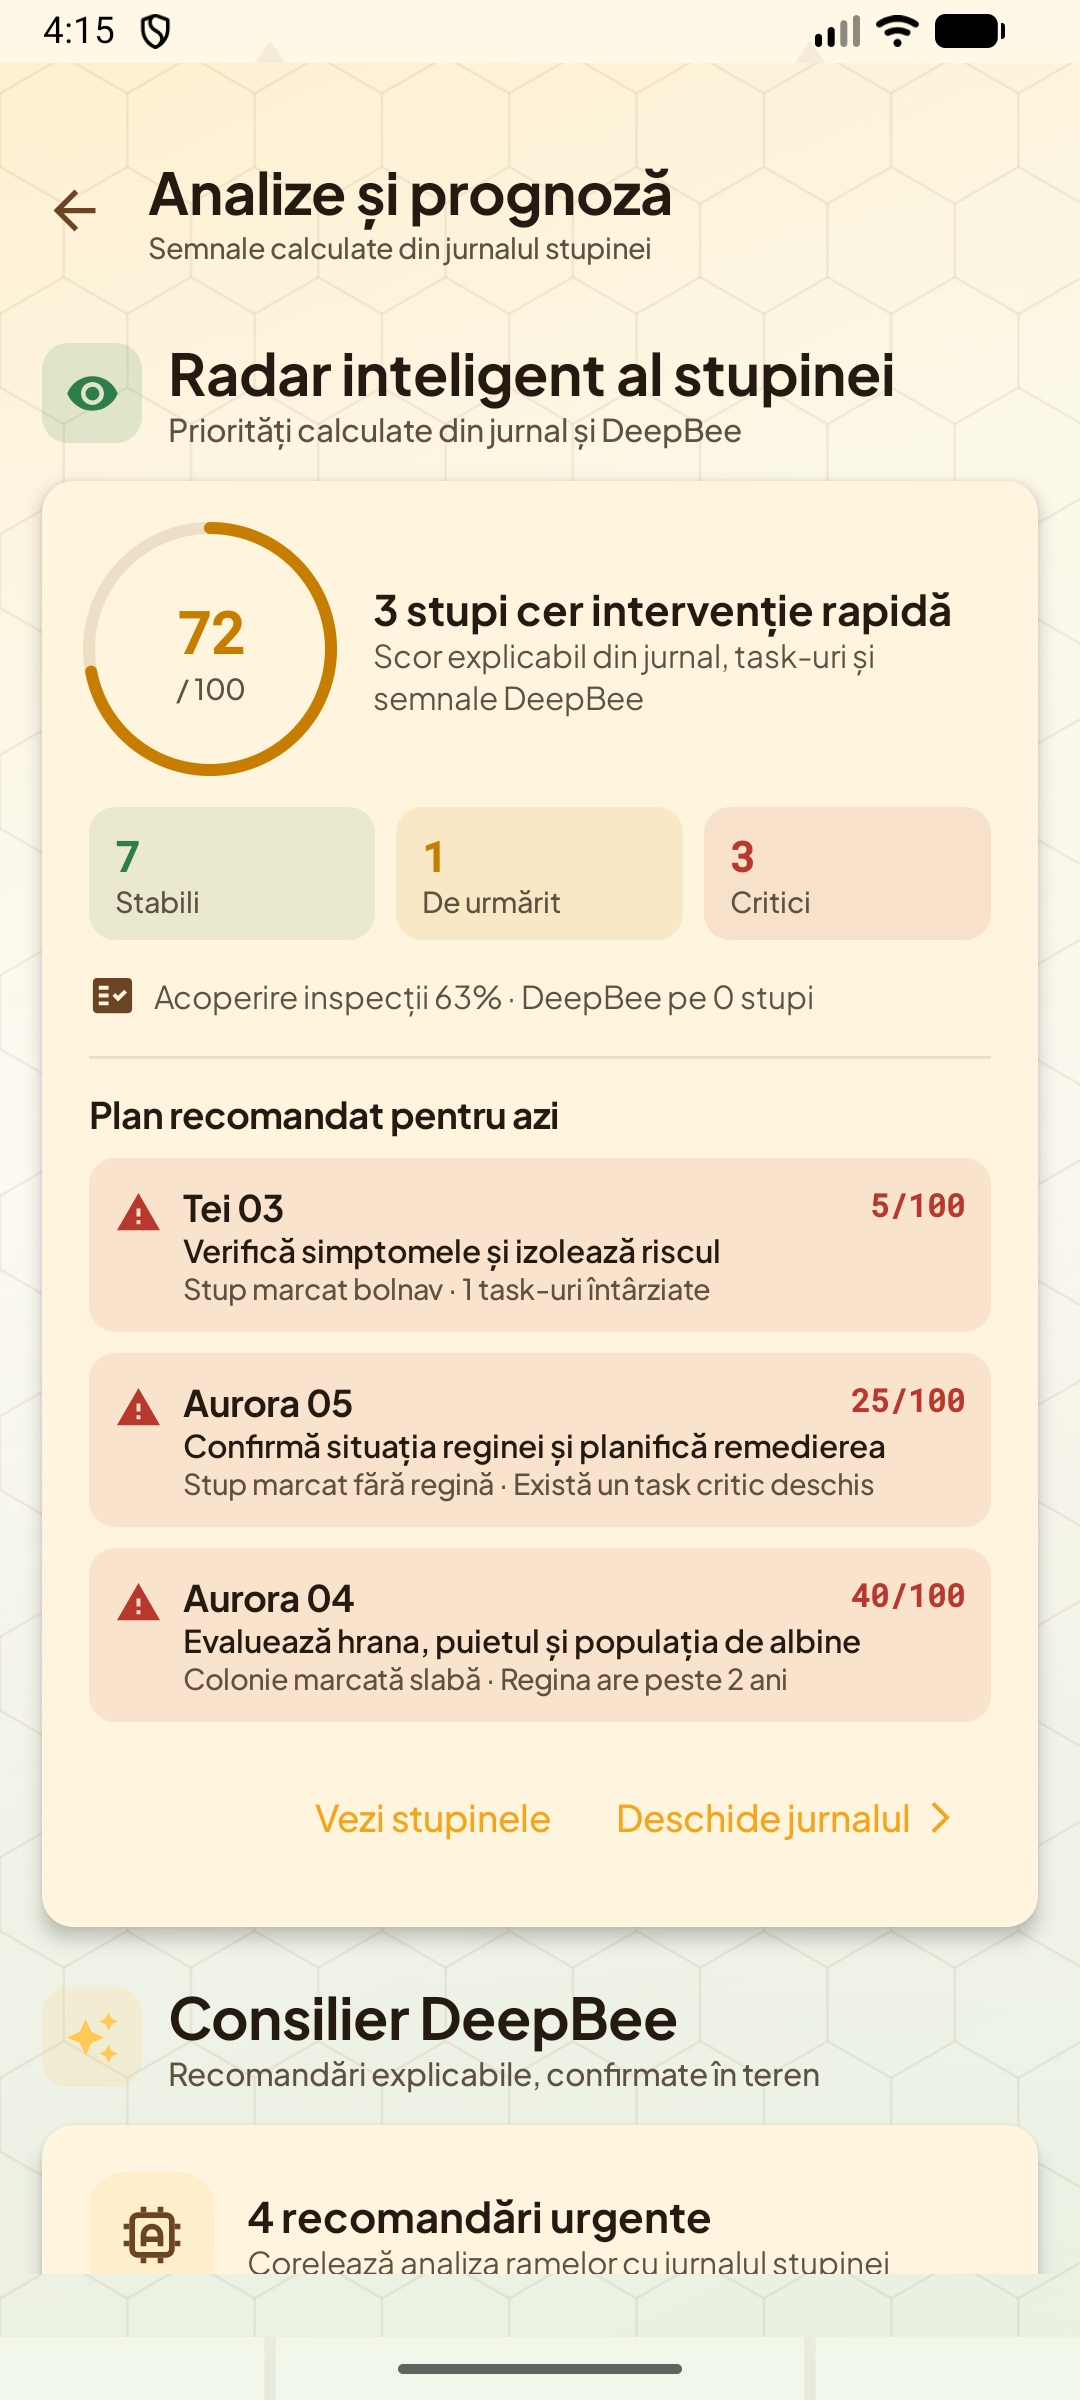
\includegraphics[width=0.40\textwidth]{./images/screenshots/dashboard-radar-updated.jpg}}
	\hfill
	\subfigure[Stupinele cu meteo și stare]{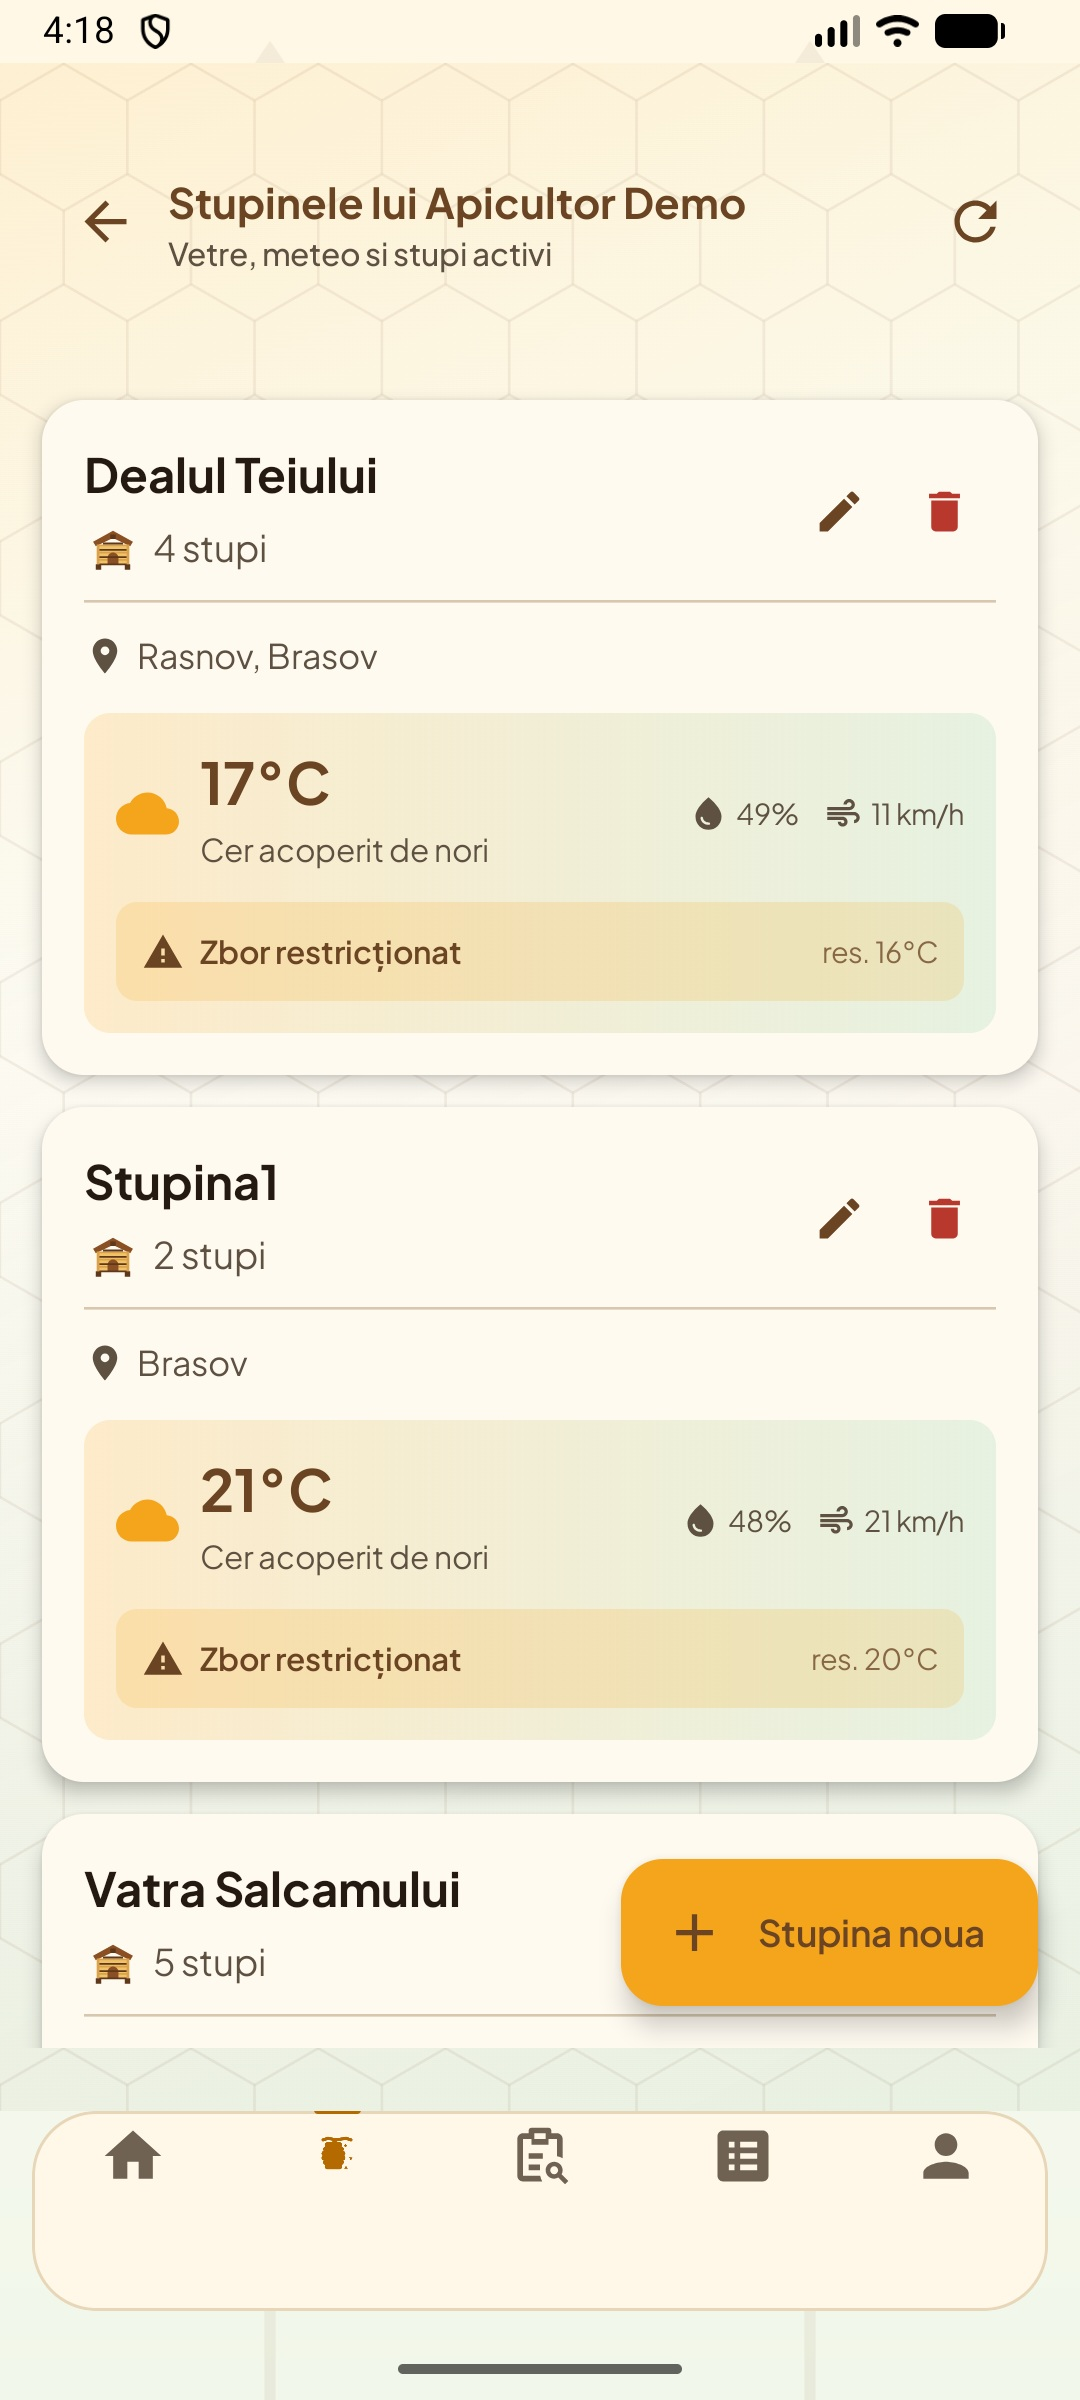
\includegraphics[width=0.40\textwidth]{./images/screenshots/14-apiaries-populated-updated.jpg}}
	\caption{Dashboard-ul cu analytics la nivel de stupină: indexul de sănătate cu planul recomandat și lista stupinelor cu date meteo contextuale.}
	\label{fig:dashboard}
\end{figure}


Un prim card afișează indexul de sănătate agregat al stupinei: scorul mediu, numărul de stupi \texttt{STABLE}, \texttt{WATCH} și \texttt{CRITICAL}, procentul stupilor cu inspecții recente și numărul celor cu cel puțin o analiză DeepBee. Sub aceste rezumate este afișată lista stupilor care necesită atenție, cu motivele penalizărilor și acțiunile sugerate.

Un al doilea card prezintă analiza de producție: producția de miere extrasă în anul curent, producția pe toată durata de viață a stupinei, prognoza pentru recolta iminentă (exprimată ca interval minim--mediu--maxim) și prognoza de sezon calculată prin adăugarea estimării ramelor cu miere la producția deja extrasă. Tendința de producție față de trimestrul anterior este exprimată procentual. Nivelul de încredere al prognozei este afișat explicit: \texttt{LOW} când datele sunt puține, \texttt{MEDIUM} sau \texttt{HIGH} pe măsură ce istoricul se acumulează.

Un al treilea card prezintă sfaturile \texttt{DeepBeeContextAdvisor}, grupate pe categorii (matcă, puiet, roire, nutriție, tratamente, producție, monitorizare, calitatea datelor) și ordonate după nivelul de urgență. Fiecare sfat include titlul, explicația, acțiunea propusă și dovezile extrase din datele aplicației. Utilizatorul poate citi sfatul și decide independent dacă îl aplică sau nu, fără ca aplicația să genereze alarme automate sau să prescrie acțiuni obligatorii. Cardurile de analytics ale dashboard-ului sunt prezentate în figura~\ref{fig:dashboard}.


\section{Tratamente, extracții și task-uri}

Tratamentele permit înregistrarea produsului administrat, substanței, dozei, datei și unei eventuale date de tratament următor. Tipurile de tratament includ, în modelul backend, Varroa, Nosema, fungal, viral, bacterial, preventive și other. Aceste informații ajută la păstrarea istoricului sanitar al stupului și sunt folosite de \texttt{DeepBeeContextAdvisor} pentru a verifica existența unui tratament Varroa înregistrat și termenele expirate.

Dacă un tratament are o dată de reaplicare, \texttt{TreatmentNotificationScheduler} programează automat o alarmă locală pentru ora 08:00 a zilei respective. Alarma supraviețuiește modului de economisire a energiei și, prin \texttt{BootCompleteReceiver}, și repornirii dispozitivului. Utilizatorul primește astfel o notificare în ziua planificată, fără a fi nevoie să verifice manual aplicația.

Extracțiile permit înregistrarea producției. Modelul include data extracției, tipul produsului, cantitatea, unitatea și notițe. Tipurile suportate includ miere, polen, propolis, lăptișor de matcă, ceară și altele. \texttt{DashboardAnalyticsCalculator} folosește înregistrările de extracții de tip \texttt{Honey} pentru calculul producției anuale și al prognozei de sezon.

Task-urile sunt folosite pentru planificarea lucrărilor. Ele pot fi asociate unei stupine sau unui stup și pot avea prioritate, status și termen limită. Pe Android, task-urile pot declanșa notificări locale prin \texttt{TaskNotificationScheduler}. De asemenea, \texttt{SyncManager} are operații speciale \texttt{COMPLETE} și \texttt{UNCOMPLETE}, pentru sincronizarea schimbării statusului unei sarcini.

\begin{figure}[H]
	\centering
	\subfigure[Task-uri prioritizate]{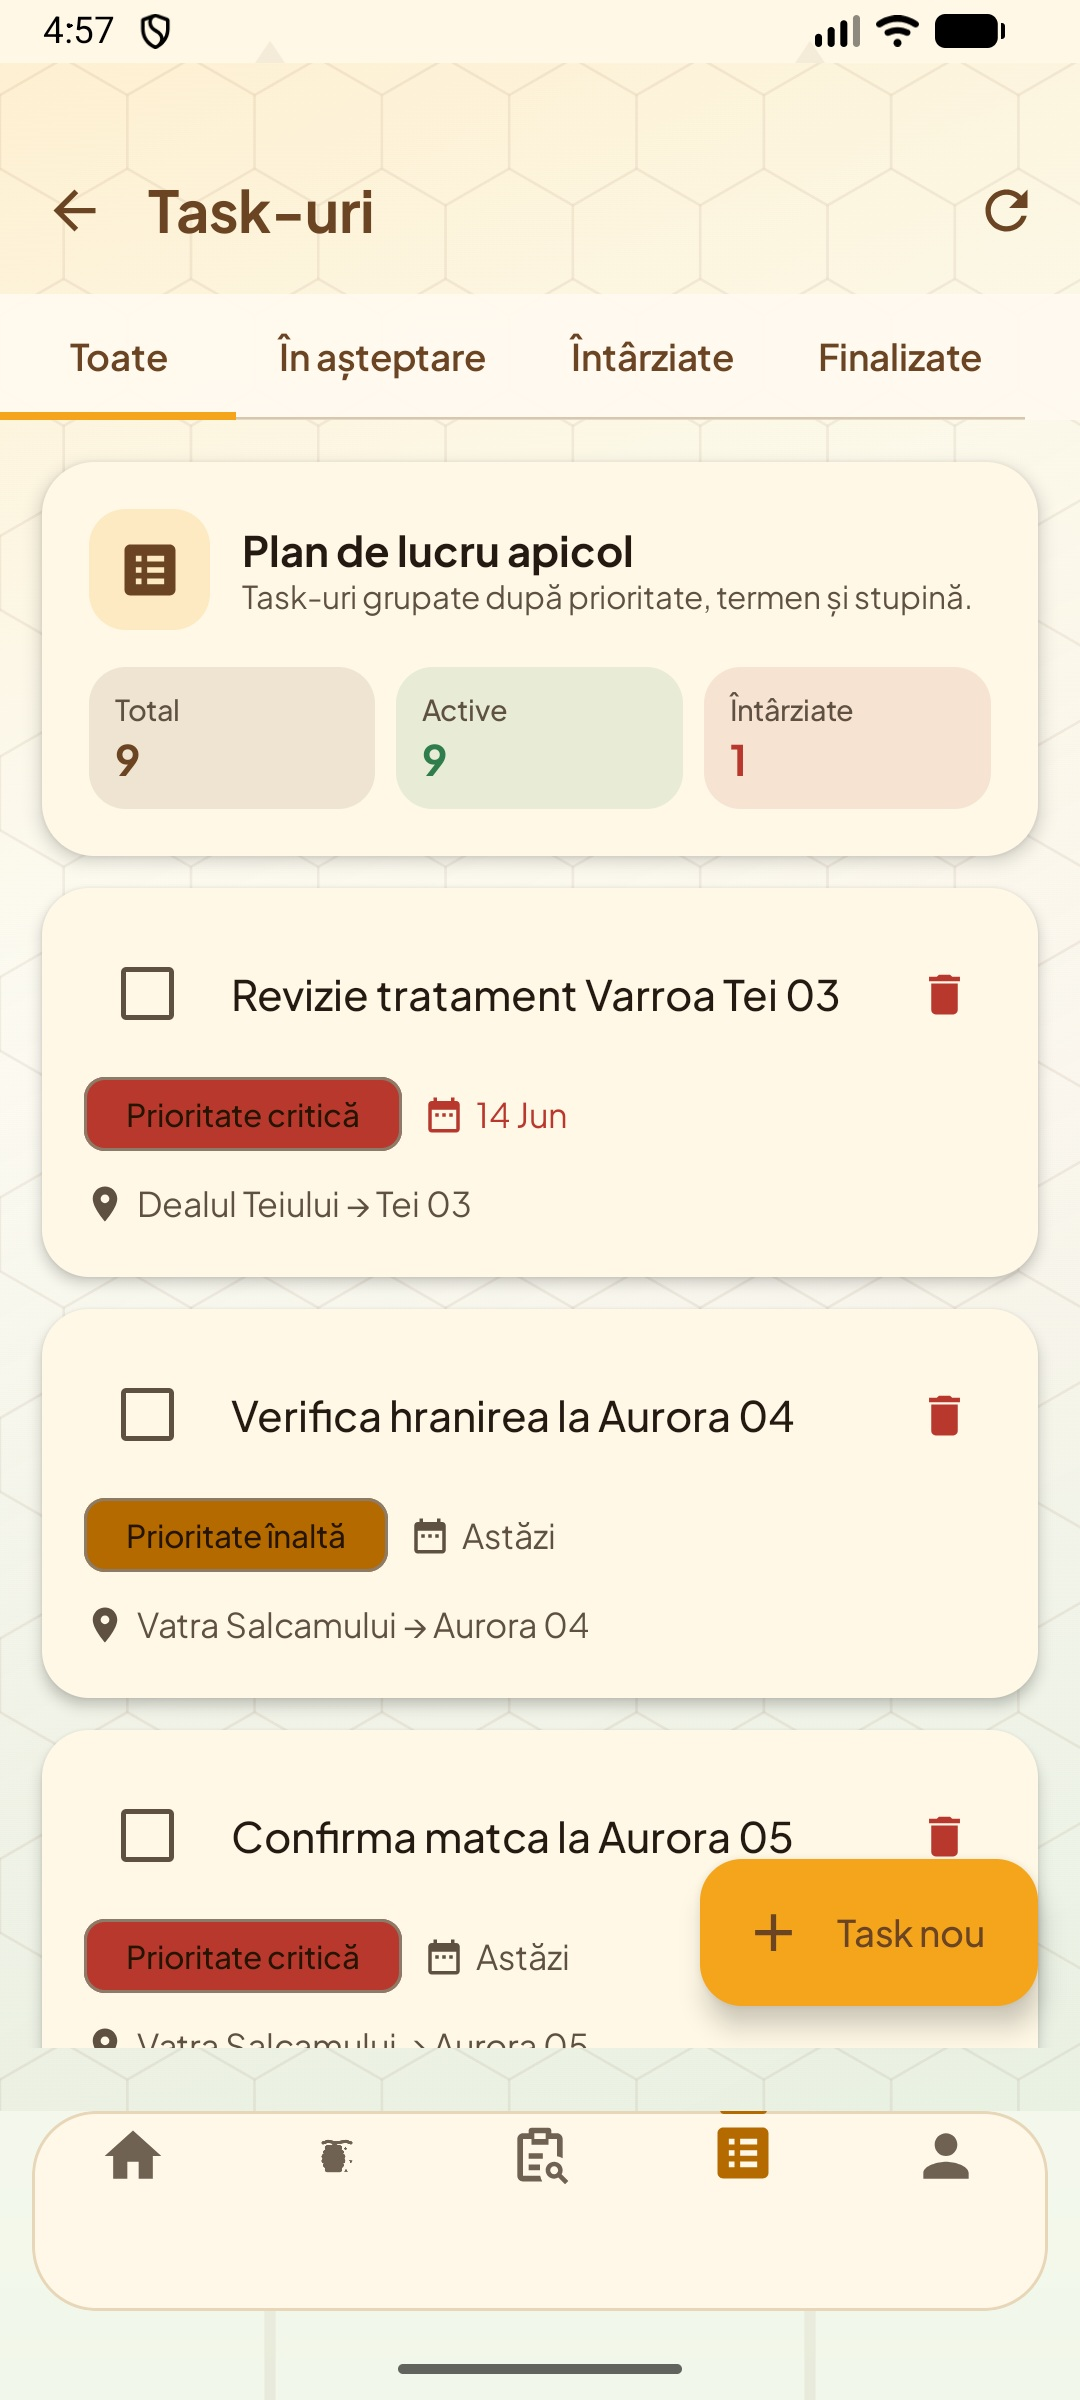
\includegraphics[width=0.40\textwidth]{./images/screenshots/task-list-updated.jpg}}
	\hfill
	\subfigure[Istoricul tratamentelor]{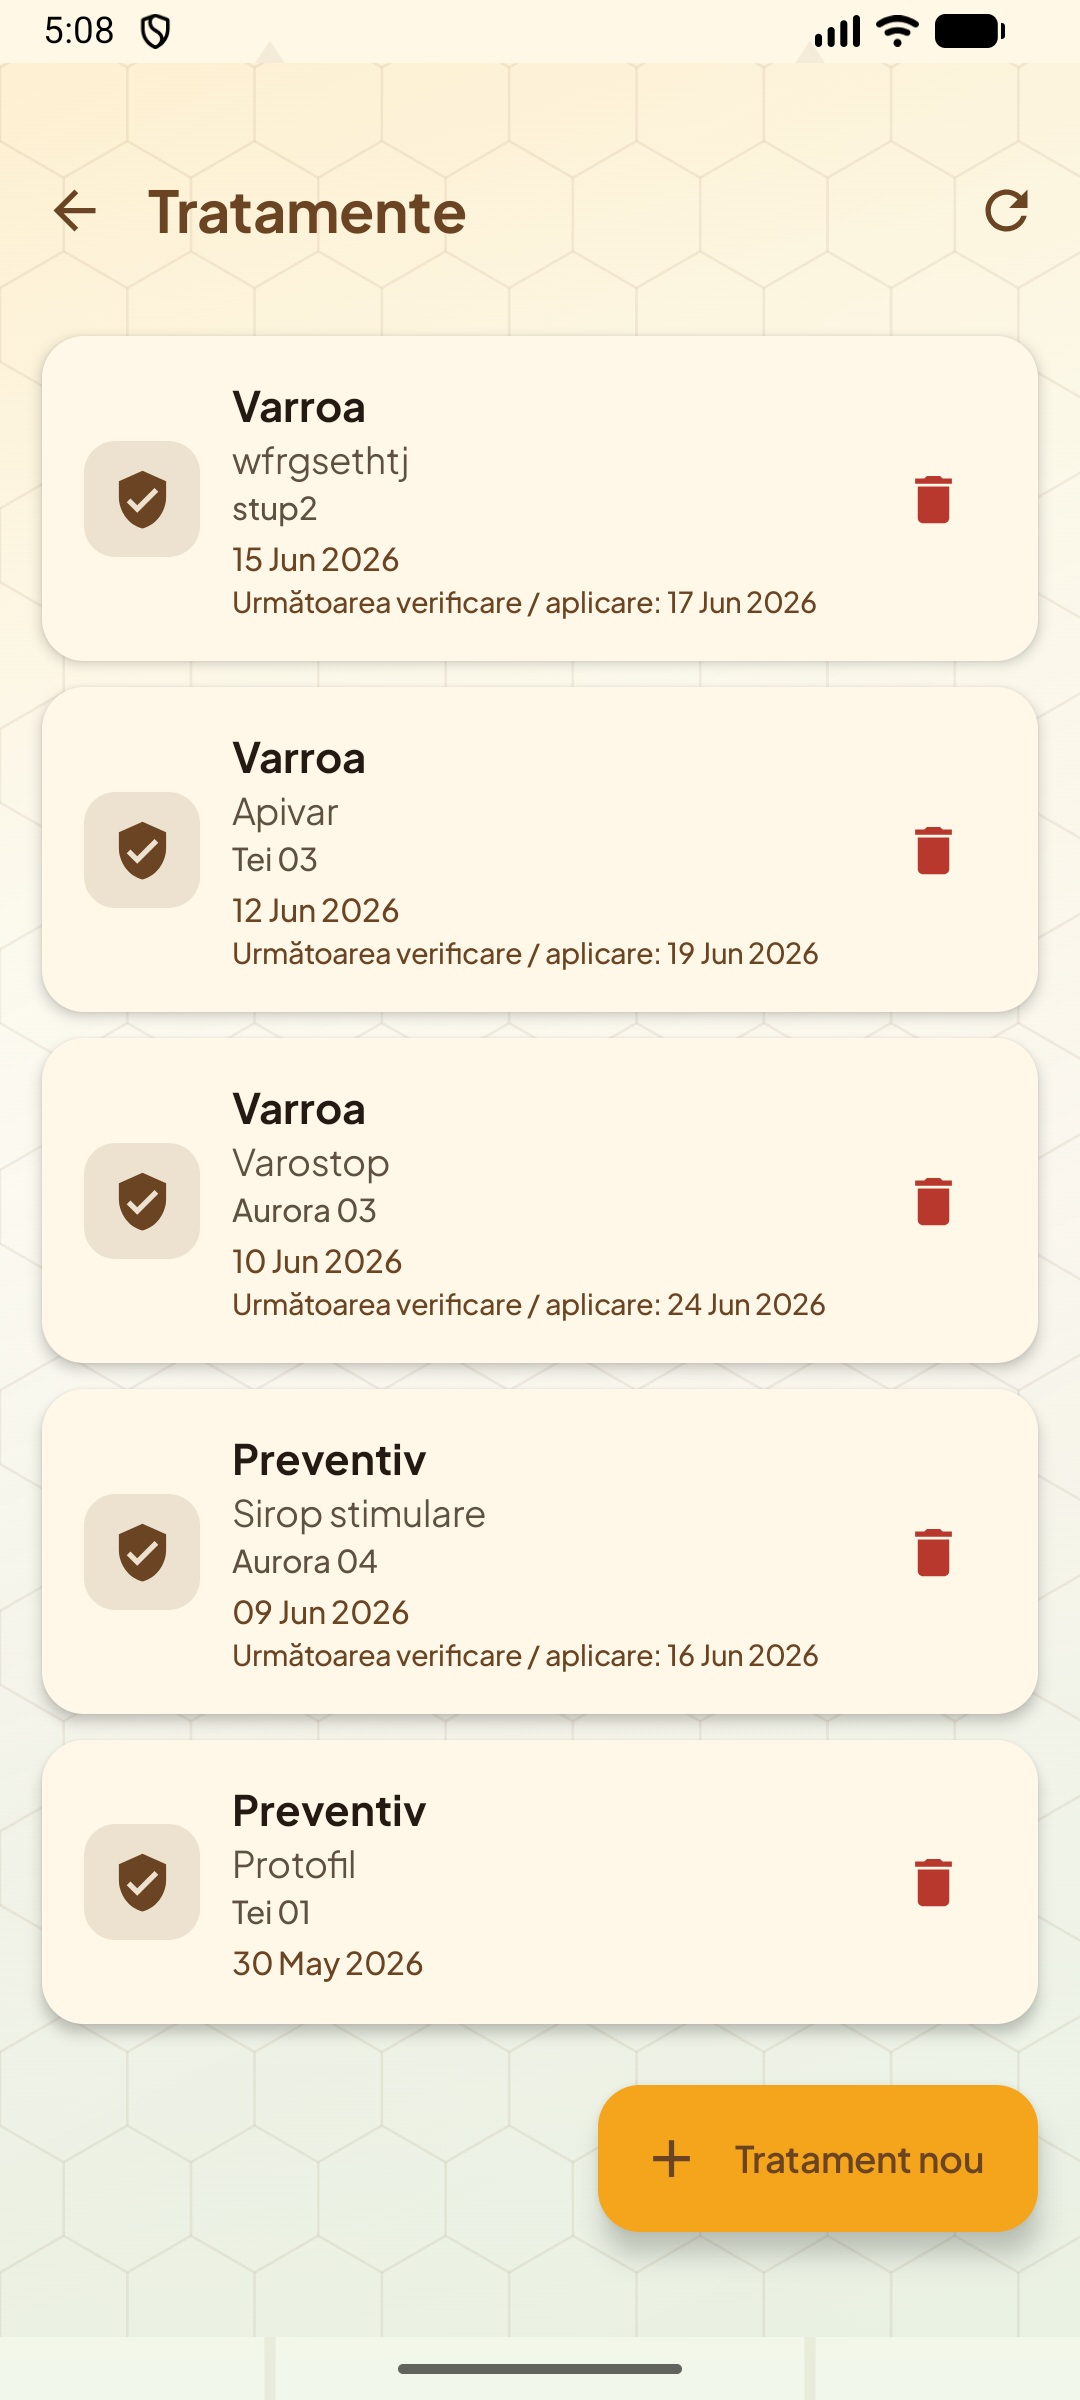
\includegraphics[width=0.40\textwidth]{./images/screenshots/treatment-list-updated.jpg}}
	\caption{Liste operaționale actualizate: task-urile sunt grupate după status și prioritate, iar tratamentele păstrează produsul, stupul, data aplicării și următoarea verificare.}
	\label{fig:worklists}
\end{figure}

\section{Funcționarea offline și sincronizarea}

Un scenariu important este lucrul complet offline. De exemplu, utilizatorul poate merge într-o stupină fără internet, poate crea o stupină nouă, adăuga doi stupi, completa inspecții și atașa fotografii. Toate aceste operații sunt salvate local. În acest timp, UI-ul nu este blocat, iar entitățile apar în liste.

Când dispozitivul revine online, \texttt{SyncScheduler} declanșează \texttt{SyncWorker}. Worker-ul apelează \texttt{SyncManager}, care procesează coada. Testele de integrare arată că ordinea este respectată: stupina este trimisă înaintea stupului, iar stupul înaintea inspecției sau fotografiei. Această ordine garantează că backend-ul primește id-uri valide.

Starea curentă a sincronizării poate fi consultată direct din ecranul de profil. \texttt{UserProfileScreen} afișează numărul de operații pendinte și momentul ultimei sincronizări confirmate cu serverul. Această informație ajută utilizatorul să știe dacă datele introduse în teren au ajuns pe server sau sunt încă în așteptare.

În cazul unei erori temporare, operația rămâne în coadă. În cazul unei erori repetate de server, entitatea este marcată \texttt{SYNC\_FAILED}. Într-o versiune viitoare, UI-ul ar putea afișa explicit o listă de operații eșuate, astfel încât utilizatorul să poată decide manual ce se întâmplă cu datele.

\section{Validare prin teste Android}

Partea Android include o infrastructură de teste orientată către sincronizarea offline-online. \texttt{SyncTestHarness} construiește o bază Room în memorie, un client Retrofit real, un MockWebServer și repository-uri reale. Astfel, testele verifică fluxul complet de la apelul repository-ului până la request-ul HTTP trimis către serverul mock.

Clasa \texttt{OfflineToOnlineSyncTest} acoperă scenarii fericite: creare de stupină offline și sincronizare, actualizare, ștergere, creare de stupină și stup în ordine de dependență, task-uri create peste părinți nesincronizați, tratamente și extracții. Clasa \texttt{SyncEdgeCasesTest} acoperă situații de eroare: retry-uri repetate, \texttt{IOException}, payload malformat, ștergeri 404, idempotency și părinți eșuați.

Pe lângă testele de integrare, există teste unitare pentru repository-uri individuale, pentru meteo, pentru \texttt{BroodAnalyzer}, pentru maparea statusurilor de analiză AI, pentru \texttt{ApiaryIntelligenceCalculator}, pentru \texttt{DashboardAnalyticsCalculator} și pentru \texttt{DeepBeeContextAdvisor}. Aceste teste verifică separat logica fiecărui calculator, inclusiv cazuri limită: stupi fără inspecții, snapshot-uri AI expirate, extracții cu unități nenormalizate, priorități de sfaturi și calendarul sezonier. Există și teste unitare pentru ViewModel-uri (\texttt{CreateApiaryViewModelTest}, \texttt{HiveFormViewModelTest}, \texttt{TaskFormViewModelTest}), care verifică comportamentul stărilor UI la acțiunile utilizatorului.

\section{Validare prin teste backend}

Backend-ul are un proiect separat de teste, \texttt{ApiaryServer.Tests}, care acoperă în prezent șapte seturi de scenarii.

Testele pentru \texttt{AuthController} verifică scenariile de înregistrare, login, confirmare email și resetare parolă, inclusiv cazuri de date invalide, email duplicat și token expirat. \texttt{AuthServiceTests} verifică logica serviciului de autentificare, inclusiv generarea și validarea token-urilor JWT și a refresh token-urilor.

Testele pentru \texttt{ApiaryService} verifică operații precum listare, creare, actualizare și ștergere, inclusiv cazul în care o stupină aparține altui utilizator. Testele pentru \texttt{HiveService} și \texttt{InspectionService} urmează același pattern: fiecare operație este testată atât pe calea fericită, cât și pentru cazurile de ownership incorect. \texttt{HiveTreatmentServiceTests} și \texttt{HiveExtractionServiceTests} verifică operațiile CRUD pe tratamente și extracții, inclusiv validarea tipurilor și a proprietarului resurselor. \texttt{TaskServiceTests} acoperă crearea, actualizarea, completarea și ștergerea task-urilor.

Testele pentru \texttt{AiAnalysisService} verifică modul în care serviciul C\# păstrează statusurile primite de la AIService. De exemplu, dacă serviciul AI întoarce \texttt{low\_quality} sau \texttt{not\_comb\_image}, backend-ul nu le transformă forțat în succes. De asemenea, dacă serviciul AI întoarce o eroare HTTP, \texttt{AiAnalysisService} aruncă o excepție care poate fi tratată de controller.

\texttt{AppDbContextModelTests} verifică că configurările de precizie zecimală din \texttt{AppDbContext} sunt aplicate corect la schema generată, astfel încât câmpurile cu mai mult de două zecimale (\texttt{BroodDensity}, \texttt{LarvaeToCappedRatio}, \texttt{StoresRatio}) să nu fie trunchiată la (18, 2) în mod implicit.

\section{Rezultate ale testării}

\begin{table}[H]
	\centering
	\begin{tabular}{l c p{4.7cm}}
		\hline
		\textbf{Suită} & \textbf{Nr. teste} & \textbf{Acoperire} \\
		\hline
		\texttt{ApiaryServer.Tests} (backend) & 101 & servicii, controllere, JWT, model BD \\
		Android (JVM / Robolectric) & 234 & sincronizare offline, repository-uri, calculatoare, ViewModel \\
		Android instrumentat & 1 & UI pe dispozitiv \\
		\hline
	\end{tabular}
	\caption{Sinteza suitelor de teste automate. Suita backend a fost executată integral (101 trecute, 0 eșuate).}
	\label{tab:teste-automate}
\end{table}

Suitele de teste automate au fost rulate înainte de predare. Proiectul de teste al backend-ului, \texttt{ApiaryServer.Tests}, a fost executat cu \texttt{dotnet test}: toate cele 101 de teste au trecut, fără niciun eșec. Suita Android, rulată cu \texttt{gradlew testDebugUnitTest}, cuprinde 234 de teste unitare și de integrare executate pe JVM (prin Robolectric și MockWebServer), plus un test instrumentat care necesită un dispozitiv sau emulator. Tabelul \ref{tab:teste-automate} sintetizează aceste suite.

Cele mai multe verificări pe Android se concentrează pe stratul de date și pe sincronizare, acolo unde o eroare ar însemna pierderea sau duplicarea datelor introduse în teren: scenariile offline-online, rezolvarea identificatorilor părinte-copil, politica de reîncercare și marcarea operațiilor eșuate. Restul suitei acoperă calculatoarele de indicatori, interceptorii de rețea și ViewModel-urile formularelor. Deoarece testele rulează pe JVM, prin Robolectric și MockWebServer, suita completă poate fi executată rapid, fără emulator, ceea ce a permis rularea ei frecventă pe parcursul dezvoltării, nu doar înainte de predare.

Pe partea de backend, ponderea mare a testelor de servicii reflectă decizia de a concentra logica de business în acest strat. Verificările de ownership apar pentru fiecare entitate, deoarece izolarea datelor între utilizatori este o cerință de securitate, nu o convenție opțională. Testele dedicate \texttt{AiAnalysisService} au un rol aparte: ele garantează că statusurile de calitate întoarse de serviciul AI ajung nealterate la client, adică exact comportamentul responsabil discutat în capitolul \ref{chap:suport-teoretic}.

\begin{table}[H]
	\centering
	\begin{tabular}{l l}
		\hline
		\textbf{Scenariu verificat manual} & \textbf{Rezultat} \\
		\hline
		Autentificare și înregistrare cont & Funcțional \\
		Dashboard cu indicatori (index de sănătate, plan recomandat) & Funcțional \\
		Listă de stupine cu date meteo contextuale & Funcțional \\
		Listă de stupi cu statusuri (activ, slab, fără regină) & Funcțional \\
		Jurnal de inspecții filtrat pe stup sau stupină & Funcțional \\
		Task-uri, tratamente și extracții populate în contul demo & Funcțional \\
		Fișa stupului și raportul longitudinal DeepBee & Funcțional \\
		Generarea codului QR pentru un stup & Funcțional \\
		Editarea profilului și sincronizarea cu serverul & Funcțional \\
		\hline
	\end{tabular}
	\caption{Scenarii verificate manual în aplicația Android, pe contul demo.}
	\label{tab:teste-manuale}
\end{table}

Tabelul \ref{tab:teste-manuale} prezintă scenariile verificate, ilustrate și de capturile din acest capitol. Verificarea manuală a fost realizată pe un telefon fizic, cu aplicația conectată la backend-ul găzduit în Azure Container Apps, deci în condiții apropiate de utilizarea reală, nu doar într-un mediu local controlat. Acest mod de testare a confirmat în special fluxurile care depind de infrastructură: autentificarea cu reîmprospătarea token-ului, încărcarea fotografiilor, analiza DeepBee parcursă integral, de la captura din telefon până la rezultatul afișat, și sincronizarea datelor după revenirea conexiunii.

Rezultatele testării arată că aplicația nu a fost verificată doar la nivel de interfață grafică, ci și la nivelul logicii interne care susține funcționarea offline-first. Acest aspect este important deoarece BeeSmart nu este o aplicație care depinde exclusiv de afișarea unor ecrane, ci un sistem în care datele parcurg mai multe etape: sunt introduse de utilizator, validate, salvate local, sincronizate cu serverul și apoi folosite în statistici, rapoarte sau fluxuri de analiză AI. Din acest motiv, testarea a urmărit nu doar confirmarea faptului că ecranele pot fi parcurse, ci și verificarea comportamentului componentelor care asigură persistența, sincronizarea și consistența datelor.

Pe partea de aplicație Android, testele confirmă faptul că repository-urile, ViewModel-urile și componentele de calcul pot trata atât situații normale, cât și situații limită. Au fost avute în vedere scenarii precum lipsa datelor, existența unor răspunsuri incomplete, snapshot-uri AI expirate, operații care trebuie păstrate pentru sincronizare ulterioară sau date locale care trebuie afișate chiar dacă serverul nu este disponibil. Aceste cazuri sunt relevante pentru o aplicație mobilă folosită în teren, deoarece utilizatorul nu lucrează întotdeauna într-un mediu controlat. Conexiunea la internet poate fi instabilă, aplicația poate fi întreruptă, iar telefonul poate reveni ulterior într-o stare în care trebuie să continue procesarea fără pierderea informațiilor introduse anterior.

Un element important verificat prin testare este comportamentul fluxului offline-first. În BeeSmart, lipsa conexiunii nu trebuie să blocheze complet utilizatorul, ci să determine salvarea locală a operațiilor și amânarea comunicării cu serverul. Testele susțin faptul că aplicația poate păstra aceste operații într-o formă structurată și le poate procesa ulterior, respectând dependențele dintre entități. De exemplu, o inspecție nu poate fi sincronizată corect dacă stupul asociat nu există încă pe server, iar o fotografie de ramă nu poate fi atașată înainte ca inspecția părinte să primească un identificator valid. Verificarea acestor situații demonstrează că sincronizarea nu este tratată ca o simplă retransmitere de cereri, ci ca un mecanism care ține cont de relațiile dintre date.

Pe partea de backend, testele validează comportamentul serviciilor care protejează datele fiecărui utilizator și aplică regulile de business ale aplicației. Verificarea ownership-ului este esențială, deoarece stupinele, stupii, inspecțiile, tratamentele și extracțiile sunt date private, asociate unui anumit cont. Prin testarea cazurilor în care o resursă aparține altui utilizator, aplicația demonstrează că regulile de acces nu depind doar de interfața mobilă, ci sunt aplicate și la nivelul serverului. Această separare este importantă din punct de vedere al securității, deoarece clientul Android nu trebuie considerat singurul responsabil pentru protecția datelor.

Testele backend au avut rolul de a verifica și comportamentul serviciilor în raport cu intrări valide și invalide. Într-o aplicație distribuită, serverul trebuie să trateze corect cererile primite, indiferent dacă acestea provin dintr-un flux normal al aplicației sau dintr-o situație excepțională. Validarea datelor, verificarea existenței resurselor, tratarea cazurilor de acces neautorizat și returnarea unor răspunsuri coerente contribuie la stabilitatea sistemului. Astfel, backend-ul nu este doar un strat de persistență, ci o componentă care impune reguli clare asupra modului în care datele pot fi create, modificate și consultate.

Validarea manuală completează testele automate prin verificarea fluxurilor în condiții apropiate de utilizarea reală. Testarea pe telefon fizic, cu backend găzduit în cloud, confirmă scenarii care nu pot fi evaluate complet prin teste unitare: autentificarea reală, încărcarea fotografiilor, apelarea serviciului AI, scanarea codurilor QR, deschiderea prin deep link și sincronizarea după revenirea conexiunii. Aceste verificări sunt importante deoarece integrează mai multe componente care, în testele automate, pot fi analizate separat. În utilizarea reală însă, aplicația Android, backend-ul, baza de date și serviciul AI trebuie să funcționeze împreună.

Un alt aspect relevant al validării manuale este observarea comportamentului aplicației din perspectiva utilizatorului final. În cazul BeeSmart, utilizatorul poate lucra într-o stupină, poate introduce date succesive despre mai mulți stupi, poate atașa fotografii și poate reveni ulterior asupra istoricului. Prin parcurgerea acestor scenarii s-a verificat dacă fluxurile sunt suficient de clare și dacă datele introduse sunt reflectate corect în ecranele de listare, detaliu, statistici și rapoarte. Astfel, testarea nu s-a limitat la corectitudinea izolată a funcțiilor, ci a urmărit și coerența experienței generale de utilizare.

Rezultatele obținute susțin ideea că BeeSmart este un prototip funcțional integrat, nu doar o colecție de componente implementate separat. Aplicația mobilă poate funcționa cu date locale, backend-ul aplică reguli de securitate și persistență, iar serviciul AI este integrat în fluxul de inspecție prin intermediul serverului. Chiar dacă există limitări care pot fi îmbunătățite în versiuni viitoare, testarea realizată oferă o bază solidă pentru concluzia că principalele obiective ale lucrării au fost atinse: digitalizarea managementului apicol, funcționarea în condiții de teren și integrarea responsabilă a analizei automate a fotografiilor de rame.

\chapter{Concluzii și perspective viitoare}
\label{chap:concluzii}

\section{Concluzii}

Lucrarea a prezentat proiectarea și implementarea BeeSmart, o aplicație mobilă offline-first pentru management apicol, integrată cu un backend ASP.NET Core, o bază de date SQL Server și un serviciu AI inspirat de DeepBee. Proiectul demonstrează că un sistem pentru apicultori poate combina evidența practică a stupilor cu funcționalități moderne precum sincronizare offline-online, deep links, scanare QR, notificări locale, meteo și analiză automată a fotografiilor de rame.

Din punct de vedere funcțional, BeeSmart acoperă fluxurile principale ale unei aplicații de management apicol: autentificare, profil utilizator, creare de stupine, adăugare de stupi, completare de inspecții, atașare de fotografii, înregistrare de tratamente și extracții, planificare de task-uri și consultarea statisticilor. Aceste funcții sunt legate între ele printr-o structură de date coerentă, astfel încât istoricul unui stup poate fi urmărit în timp.

Din punct de vedere tehnic, contribuția principală este arhitectura offline-first. Room permite salvarea locală a datelor, iar \texttt{SyncQueueEntity} păstrează operațiile care trebuie trimise ulterior la server. \texttt{SyncManager} procesează coada în ordinea dependențelor, ceea ce permite crearea offline a unor lanțuri de date, cum ar fi stupină - stup - inspecție - fotografie. Această abordare este potrivită pentru apicultură, deoarece lucrul în teren nu garantează conexiune permanentă la internet.

Integrarea AI adaugă o direcție suplimentară de valoare. Fotografia de inspecție nu este doar arhivată, ci poate fi analizată pentru obținerea unei distribuții de celule. Rezultatele sunt transformate în indicatori precum puiet, rezerve, densitate de puiet și raport larve/puiet căpăcit. Astfel, aplicația poate oferi un suport decizional orientativ, fără a înlocui observația apicultorului sau diagnosticul veterinar.

\section{Avantajele aplicației}

Principalele avantaje ale aplicației sunt:
\begin{itemize}
	\item centralizarea datelor despre stupine, stupi și intervenții;
	\item funcționarea offline și sincronizarea automată ulterioară;
	\item păstrarea fotografiilor de inspecție în contextul inspecției;
	\item integrarea analizei DeepBee în fluxul aplicației;
	\item statistici longitudinale pe stup și indicatori derivați;
	\item organizarea task-urilor și notificări locale;
	\item acces rapid la stup prin cod QR și deep links;
	\item suport pentru meteo pe baza locației stupinei;
	\item interacțiune prin introducere vocală pentru completarea formularelor.
\end{itemize}

Un alt avantaj este separarea clară între client, backend și serviciul AI. Această separare face proiectul extensibil. De exemplu, serviciul AI poate fi îmbunătățit fără rescrierea aplicației Android, iar backend-ul poate fi scalat sau mutat într-un mediu cloud fără modificarea majoră a interfeței.

\section{Limitări actuale}

Aplicația are și limitări care trebuie menționate. În primul rând, analiza AI depinde de calitatea fotografiei. O imagine neclară, prea întunecată sau care nu surprinde frontal fagurele poate produce un rezultat slab sau poate fi respinsă. Deși serviciul AI include praguri de calitate, acest lucru nu elimină complet riscul interpretărilor incorecte.

În al doilea rând, stocarea fotografiilor ca Data URI/Base64 este potrivită pentru prototip și demonstrație, dar nu este ideală pentru producție. O variantă mai robustă ar fi folosirea unui serviciu de stocare a obiectelor și salvarea în baza de date doar a metadatelor și a URL-urilor.

În al treilea rând, rezolvarea conflictelor între mai multe dispozitive nu este complet implementată. Aplicația gestionează bine operațiile offline pe un singur dispozitiv, dar scenariile în care mai mulți utilizatori sau mai multe dispozitive modifică aceleași date necesită reguli suplimentare.

În al patrulea rând, testarea interfeței grafice nu este complet automatizată. Repository-ul conține teste solide pentru sincronizare și servicii, însă o versiune matură ar trebui să includă teste UI, teste instrumentate pe dispozitive reale și validare mai extinsă a serviciului AI pe imagini variate de rame.

În al cincilea rând, în stadiul actual de dezvoltare clienții HTTP ai aplicației Android (\texttt{UnauthenticatedClient} și \texttt{AuthenticatedClient}) sunt configurați să accepte toate certificatele TLS, printr-un \texttt{TrustManager} permisiv (\texttt{TrustAllCerts}). Această alegere a simplificat testarea împotriva backend-ului local și a celui găzduit, dar dezactivează validarea lanțului de certificate și expune comunicarea unui posibil atac de tip man-in-the-middle. Pentru o versiune de producție, această configurație trebuie înlocuită cu validarea standard a certificatelor emise de o autoritate de încredere și, ideal, cu certificate pinning pentru domeniile cunoscute ale backend-ului.

\section{Perspective viitoare}

O direcție naturală de dezvoltare este îmbunătățirea modelului AI. Serviciul actual poate fi extins cu o implementare mai completă a segmentării semantice, cu modele antrenate pe imagini locale și cu evaluare sistematică pe seturi de test. De asemenea, modelul ar putea returna nu doar număr de celule pe clasă, ci și coordonate, scoruri de încredere și hărți vizuale peste imagine.

O altă direcție este introducerea predicțiilor privind evoluția stupului. Pe baza istoricului de inspecții, tratamente, extracții, meteo și analize AI, aplicația ar putea estima dacă o colonie are o evoluție pozitivă sau dacă există semnale de scădere. Aceste predicții ar trebui tratate ca recomandări orientative și validate pe date reale.

Pentru apicultorii cu multe stupine, un dashboard web ar fi util. Acesta ar putea afișa hărți, rapoarte, grafice comparative și alerte la nivel de stupină. Backend-ul existent ar putea susține o astfel de extensie, deoarece expune deja API-uri REST și persistă datele centralizat.

Alertarea inteligentă este o altă direcție posibilă. În forma actuală, notificările sunt locale și orientate către task-uri. În viitor, sistemul ar putea genera alerte pe baza condițiilor meteo, a termenelor de tratament, a datelor istorice și a rezultatelor AI. De exemplu, o scădere repetată a indicatorului de puiet ar putea genera o alertă de verificare.

Integrarea senzorilor IoT este, de asemenea, o dezvoltare potrivită pentru BeeSmart. Date precum temperatura internă a stupului, umiditatea, greutatea sau sunetul coloniei ar putea completa inspecțiile manuale. O astfel de integrare ar transforma aplicația într-un sistem de monitorizare mai amplu, nu doar într-o aplicație de evidență.

În final, aplicația ar putea susține partajarea datelor cu alți apicultori, consultanți sau medici veterinari. Această funcție ar necesita un model de permisiuni mai complex, dar ar putea crește utilitatea aplicației în ferme apicole mai mari sau în contexte de colaborare.

\section{Concluzie finală}

BeeSmart demonstrează că o aplicație de management apicol poate fi construită prin integrarea unor tehnologii moderne într-o arhitectură coerentă. Lucrarea îmbină dezvoltarea Android, backend-ul web, persistarea datelor, sincronizarea offline-first și analiza automată a imaginilor. Rezultatul este un prototip funcțional, cu utilitate practică pentru apicultori și cu direcții clare de extindere.

Prin modul în care leagă observațiile manuale, fotografiile, analiza AI și istoricul stupului, BeeSmart propune un model de aplicație în care tehnologia nu înlocuiește experiența apicultorului, ci o completează. Acesta este, de fapt, obiectivul central al proiectului: transformarea datelor colectate în teren în informații organizate, persistente și utile pentru decizii mai bune.


\printbibliography[title=Bibliografie]

% Raport de similaritate Turnitin (paginile 1, 2 și 3), atașat după bibliografie
\clearpage
\thispagestyle{empty}
\begin{center}
	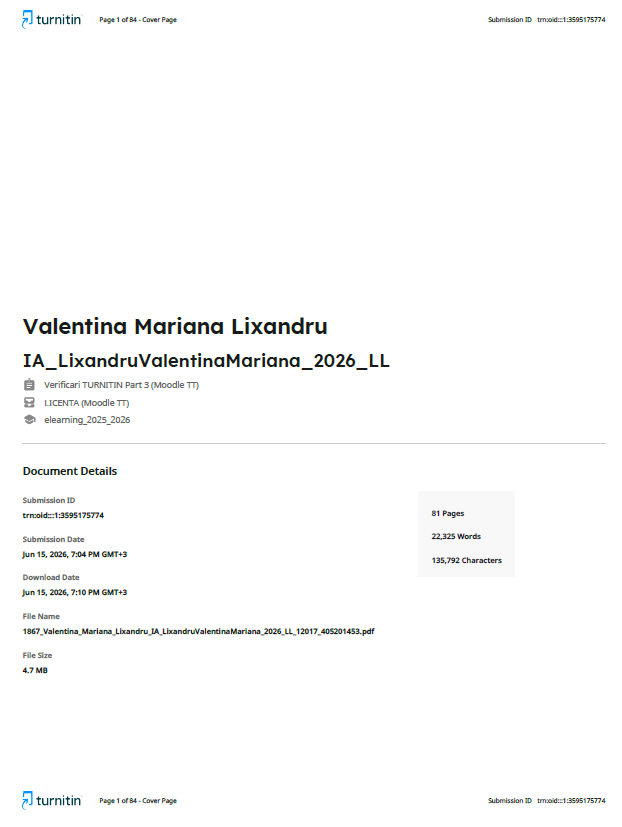
\includegraphics[height=0.96\textheight,width=\textwidth,keepaspectratio]{./images/raport-similaritate-p1.png}
\end{center}
\clearpage
\thispagestyle{empty}
\begin{center}
	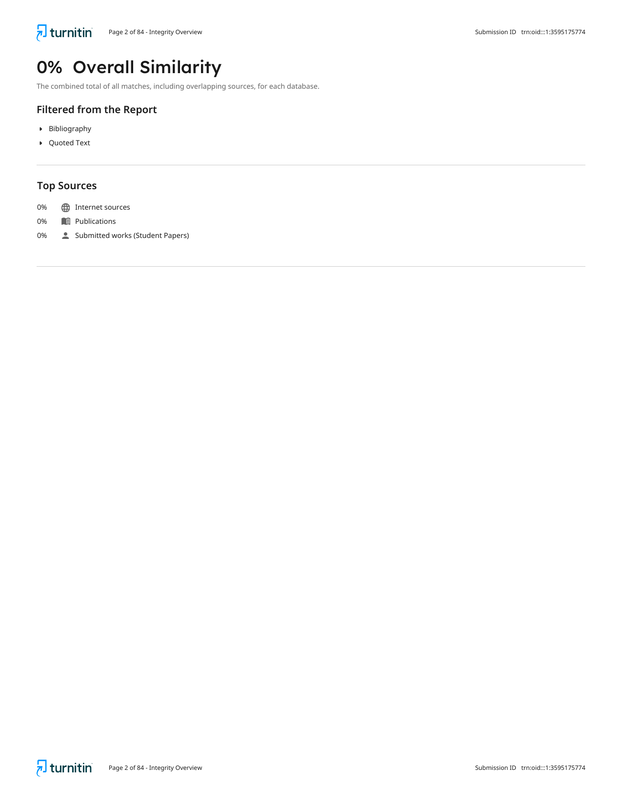
\includegraphics[height=0.96\textheight,width=\textwidth,keepaspectratio]{./images/raport-similaritate-p2.png}
\end{center}
\clearpage
\thispagestyle{empty}
\begin{center}
	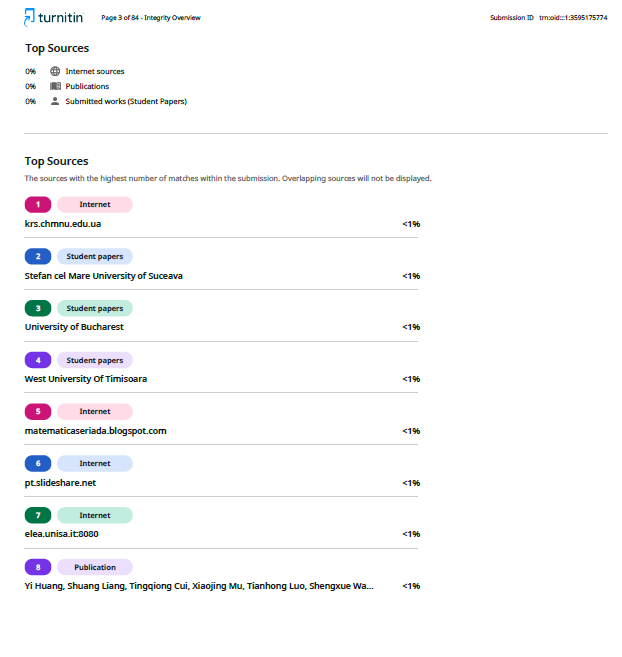
\includegraphics[height=0.96\textheight,width=\textwidth,keepaspectratio]{./images/raport-similaritate-p3.png}
\end{center}

\end{document}
